% !Mode:: "TeX:UTF-8"
%!TEX program  = xelatex

% \documentclass{cumcmthesis}
\documentclass[withoutpreface,bwprint]{cumcmthesis} %去掉封面与编号页

\usepackage{url}
\usepackage{graphicx}
\usepackage{float}
\usepackage{threeparttable}
\usepackage{subfig}
\usepackage{tabularx}
\usepackage{array}
\usepackage{caption}

\newcolumntype{C}{>{\centering\arraybackslash}X}
\captionsetup[table]{aboveskip=0pt, belowskip=0pt} 

\title{基于因果预测与滚动随机预测的微网购电优化模型}
\tihao{C}
\baominghao{4321}
\schoolname{XX大学}
\membera{zstar}
\memberb{向左}
\memberc{哈哈}
\supervisor{老师}
\yearinput{2021}
\monthinput{08}
\dayinput{22}

\begin{document}

\maketitle
\begin{abstract}

本文聚焦微网在不确定光伏与电价环境下的外网购电优化，针对信息预测不确定性与决策复杂度逐级递增的结构，建立了从确定性日前线性计划到滚动随机规划的决策模型。

\textbf{针对问题一：}由于分时电价、小区负载及光伏发电预测功率均不随日期变化，分析三者存在早上价格低、负载高，午间“双低”、晚间“双高”的特征，再根据能量守恒等约束建立线性规划求解模型，按储能不同时充放电原则加入惩罚项，求得全天最优购电费用 35126.95 元、全天购电量 59482.70 kWh 及全天各时段数据，并通过敏感性分析验证同时充放电惩罚系数 $10^{-8}$ 不影响购电结果。

\textbf{针对问题二：}在问题一基础上，考虑小区负载与光伏发电功率随日期变化、紧急购电为正常电价 5 倍的情形，构建因果多步 Fourier 岭回归预测模型，通过加权损失抑制光伏高估；生成并压缩连续三日误差场景，叠加低光伏压力场景与场景树非预见性约束，建立三日滚动风险感知随机规划模型，按实际光伏因果滚动执行。全年计划购电费用 12,905,515.22 元、紧急购电费用 825,521.25 元，总费用 13,731,036.47 元，给出指定日期紧急购电情况，验证了风险权重0.25设置的合理性。

\textbf{针对问题三：}在问题二基础上，本文遵循“基准电量按电价结算、少购部分半价、多购部分 1.5 倍价”建立“日前计划—日内多阶段调整—10 分钟滚动执行”三层随机优化模型。每天 00:00制定日前计划购电量，依据更新预报对尚未发生的时段重新优化调整购电量；每 10 分钟滚动执行储能充放电、弃光和紧急购电，并引入历史预报误差分位数修正、场景压缩、CVaR 风险度量及非预见性约束。得全年总购电费约为 13,922,405.25 元，紧急购电量约为 61,376.99 kWh；总费用较问题二上升约 1.39\%，但紧急购电量下降约 61.63\%；保留四次更新较仅 00:00 更新总费用降低 51.19 万元、紧急购电量降低约 18.39 万 kWh，凸显日内更新的价值。

\textbf{针对问题四：}在问题二、三基础上，引入波动电价，研究日前计划购电与“计划 + 滚动调整”购电优化，考虑光伏与价格残差的反相关，构建光伏-价格联合风险预测；再以 Fourier 岭回归与同星期日曲线校正进行严格因果预测，并以多层结构生成与更新策略。重做的问题三（下称问题四-3）相比重做的问题二（下称问题四-2），全年总费用从 1,525.92 万元降至 1,463.56 万元，紧急购电量从 339,672.51 kWh 降至 92,397.77 kWh，下降72.80\%；消融实验显示去除光伏-价格联合场景会显著改变代表日成本结构，总费用从 37,619.52 元骤降至 24,561.11 元，取消日内更新使问题四-3代表日总费用下降 859.14 元，但紧急购电量增加 45.66 kWh，说明日内更新体现总费用与供电风险的权衡，验证了联合场景与滚动更新的有效性。


\keywords{\quad 微电网优化 \quad 因果预测 \quad 滚动随机规划 \quad CVaR 风险度量}
\end{abstract}
%目录（可要可不要）
%\tableofcontents


\section{问题重述}

\subsection{问题背景}
微网能高效集成各类负载、分布式可再生能源及储能系统，并通过从外网购电维持本地用电平衡。外网电价较低或者分布式能源产电过量时，微网可以通过整体调控将电力存入储能装置；电价较高或者分布式能源产电不足时则调节储能装置放出电力。

微网系统在助力能源系统向低碳、绿色转型中发挥着基石性的作用，不过分布式能源产电的时间不确定性导致能源管理的不确定因素不断增加，需要建立更好的外网购电与储能装置充放电规划，以在保障用户需求同时力求节省购电费用。

\subsection{问题要求}
题目给出了储能设备的各项指标以及不同背景下的电价、小区负载和光伏发电功率，要求我们根据附录和附件1-4中给出的数据，建立数学模型，求解如何制定微网每天的购电策略，并进行分析。

\textbf{问题一：}在\textbf{每天的电价与小区负载均不变并给出}、\textbf{光伏发电功率随时间变化并给出预测值}的条件下，在每天0：00制定当天计划购电策略使得总购电费用最小，并研究在指定时间段及全天的购电量、购电费用、储能装置充放电量。其中，微网提供的电能必须时刻足够用于负载，储能设备在一天结束时需回到初始储存量。

\textbf{问题二：}保持\textbf{每天的电价不变并给出}，改为\textbf{小区负载随时间变化并给出、光伏发电功率随时间变化并给出真实值}，并引入当微网提供电量不足以供给小区负载时以5倍实时电价进行紧急购电的惩罚因素，在从2月1日开始一直到年末每天0：00指定当天的微网\textbf{计划购电与紧急购电策略}以最小化预期费用，并给出3月20日、6月21日、9月23日、12月21日四个指定日期的紧急购电量。

\textbf{问题三：}\textbf{在第二问的条件下}，新增\textbf{每天四次的光伏发电预报}，并引入计划购电量高于调整购电量时的半价违约罚款、调整购电量高于计划购电量时的1.5倍购入惩罚，从2月1日开始直到12月31日每天0:00制定当天的\textbf{计划购电与紧急购电策略}，在其他预报时刻制定\textbf{调整购电策略}。此外，分析是否有必要新增其他时刻的预报来优化购电策略的制定。

\textbf{问题四：}在\textbf{电价、小区负载、光伏发电功率均变化并给出}的前提下，重新研究问题二、三的购电策略。

四问层层递进，不断引入新条件，核心研究问题均为\textbf{在保证供电的前提下，如何制定购电策略来最小化总购电费用}。

\section{模型假设}

\begin{enumerate}
  \item 将一天划分为 144 个 10 分钟时段，此时段为最小时间单位，假设时段内电价、小区负载、光伏发电及其决策量不变，且微网满足能量守恒，不计入题目要求外的损耗；
  \item 时段内的充放电、购电量在时段初立即实现，不考虑设备启停、通信或控制延迟。
  \item 问题一中，假设电价、小区负载始终完全已知；光伏发电预测功率即为实际功率，始终完全已知；
  \item 问题二与问题三中，假设电价、小区负载始终完全已知；对某个时段，当前时段之前的光伏发电实际功率已知，当前时段之后的光伏发电实际功率未知；
  \item 问题四中，假设小区负载始终完全已知；对某个时段，当前时段之前的电价、光伏发电实际功率已知，当前时段之后的电价、光伏发电实际功率未知。
\end{enumerate}

\section{符号说明}

本文涉及的主要变量符号汇总如下。未在表中声明的局部符号在首次出现处说明。

\begin{table}[H]
  \centering
  \caption{主要符号说明}
  \label{tab:symbols}
  \small
  \begin{tabularx}{\textwidth}{cXc}
    \toprule
    符号 & 说明 & 单位 \\
    \midrule
    $t$ & 一天内的 10 分钟时段序号，$t=1,\dots,144$ & -- \\
    $L_t$ & 第 $t$ 个时段的负载电量 & kWh \\
    $R_t$ & 第 $t$ 个时段的实际光伏电量 & kWh \\
    $\hat R_t$ & 光伏预测电量（问题一为点预测，问题三为复合预测） & kWh \\
    $P_t$ & 日前计划购电量（问题一中为光伏预测电量） & kWh \\
    $A_t$ & 日内更新后的最终调整购电量（问题三/四） & kWh \\
    $u_t,v_t$ & 计划相对调整的过剩/不足量，$u_t=(P_t-A_t)^+$, $v_t=(A_t-P_t)^+$ & kWh \\
    $G_t$ & 问题一中外网购电量 & kWh \\
    $c_t,d_t$ & 储能充电量、放电量 & kWh \\
    $e_t$ & 紧急购电量 & kWh \\
    $s_t$ & 储能荷电状态（SOC） & kWh \\
    $p_t$ & 时段电价；紧急购电价格为 $5p_t$ & 元/kWh \\
    $C_t^{\rm normal}$ & 主结算费用（问题三/四） & 元 \\
    $\eta$ & 储能充放电单向效率，取 $0.90$ & -- \\
    $\lambda$ & CVaR 风险惩罚权重，取 $0.25$ & -- \\
    $\alpha$ & CVaR 置信水平，取 $0.90$ & -- \\
    $\mathrm{CVaR}_\alpha(\cdot)$ & 条件风险价值 & -- \\
    MAE/RMSE & 平均绝对误差/均方根误差 & kW \\
    \bottomrule
  \end{tabularx}
\end{table}


\section{问题一：基于线性规划每日购电策略模型}
\subsection{问题分析}

在第一问中，电价、小区负载以及光伏发电预测功率均已知。光伏发电的预测功率会带来微网预测提供电量的偏差，为简化模型，在这里我们假设由预测误差带来的不确定性\textbf{可忽略}，求解结束后再判断是否出现微网预测提供电量不小于小区负载，实际却远小于小区负载的情况。

决策核心在于：在每个 10 min 内，通过协调外网购电量与储能装置的充放电量，不仅要使得全天购电总费用最小，还要在每一个十分钟都满足负载供需平衡、储能在限制范围以内以及首尾 SOC （储能装置电荷量）一致等条件。故问题一属于\textbf{优化问题}。

由于除储能装置尽量不同时充放电的非线性约束外，目标函数与约束条件均为线性，线性约束条件参数均已知，故问题一可先建模成\textbf{线性规划（LP）问题}，后在目标函数中加入极小的充放电\textbf{惩罚项}，在不改变主要经济结果的前提下有效简化求解过程。

\subsection{数据预处理}

问题一所用附件1的数据类型有时间、电价、小区负载“光伏发电功率”四列，每列数据144行，每10分钟为一个最小时间单位呈现各项数据，对附件1做如下数据预处理：

\subsubsection{数据来源与字段说明}

一天划分为 $t=1,2,\ldots,144$ 共 144 个十分钟时段，每个时段长度：
\[
\Delta t=\frac{10}{60}=\frac16\ \mathrm{h}.
\]
第 $t$ 个时段对应当天 0:00 起算的第 $t$ 个十分钟区间：
\[
I_t=[10(t-1),\,10t)\ \text{分钟},\quad t=1,2,\ldots,144.
\]
其中 $t=1$ 为 $0:00$--$0:10$，$t=144$ 为 $23:50$--$24:00$，后续直接以编号 $t$ 为时间索引。

处理后数据包含8个数据类型，各数据含义及作用见表\ref{tab:q1-fields}。

\begin{table}[H]
  \centering
  \caption{问题一预处理后数据属性列说明}
  \label{tab:q1-fields}
  \small
  \begin{tabularx}{\textwidth}{CCCC}
    \toprule
    字段 & 含义 & 单位或范围 & 建模作用 \\
    \midrule
    \texttt{t} & 时段编号 & $1,\ldots,144$ & 核心时间索引 \\
    \texttt{price} & 分时电价 & 元/kWh & 购电成本目标函数表示符 \\
    \texttt{load\_kw} & 小区负载功率 & kW & 绘制功率曲线及校验范围 \\
    \texttt{pv\_kw} & 光伏预测功率 & kW & 绘制功率曲线、校验范围 \\
    \texttt{load\_kwh} & 十分钟负载电量 & kWh & 能量平衡约束表示符 \\
    \texttt{pv\_kwh} & 十分钟光伏电量 & kWh & 能量平衡约束表示符 \\
    \texttt{net\_load\_kw} & 净负载功率 & kW & 净负载曲线、功率检查 \\
    \texttt{net\_load\_kwh} & 十分钟净负载电量 & kWh & 作为净负载输入 \\
    \bottomrule
  \end{tabularx}
\end{table}

数据校验与异常值处理检验时序合理、数值合法。

\subsubsection{单位换算与建模参数构造}

原始数据中的功率单位为 kW，需统一以 kWh 为单位。设第 $t$ 个时段的负载功率和光伏功率分别为 $L_t^{\mathrm{kw}}$、$P_t^{\mathrm{kw}}$，则对应电量为
\[
L_t=L_t^{\mathrm{kw}}\Delta t=\frac{L_t^{\mathrm{kw}}}{6},\quad
P_t=P_t^{\mathrm{kw}}\Delta t=\frac{P_t^{\mathrm{kw}}}{6}.
\]

净负载先在功率层面计算，再换算为电量：
\[
N_t^{\mathrm{kw}}=L_t^{\mathrm{kw}}-P_t^{\mathrm{kw}},\quad
N_t=N_t^{\mathrm{kw}}\Delta t=L_t-P_t.
\]

这里需要特别说明：净负载反映的是本地负载与光伏之间的供需缺口或光伏富余，\textbf{与是否从外部电网购电无关}。

其中 $N_t>0$ 表示光伏不足以供给负载，$N_t<0$ 表示光伏有富余。

\subsubsection{数据特征可视化}

为直观分析小区负载、光伏出力及分时电价的日内变化规律，绘制图 \ref{fig:q1_1} 如下。

\begin{figure}[H]
    \centering
    \subfloat[全天分时电价曲线]{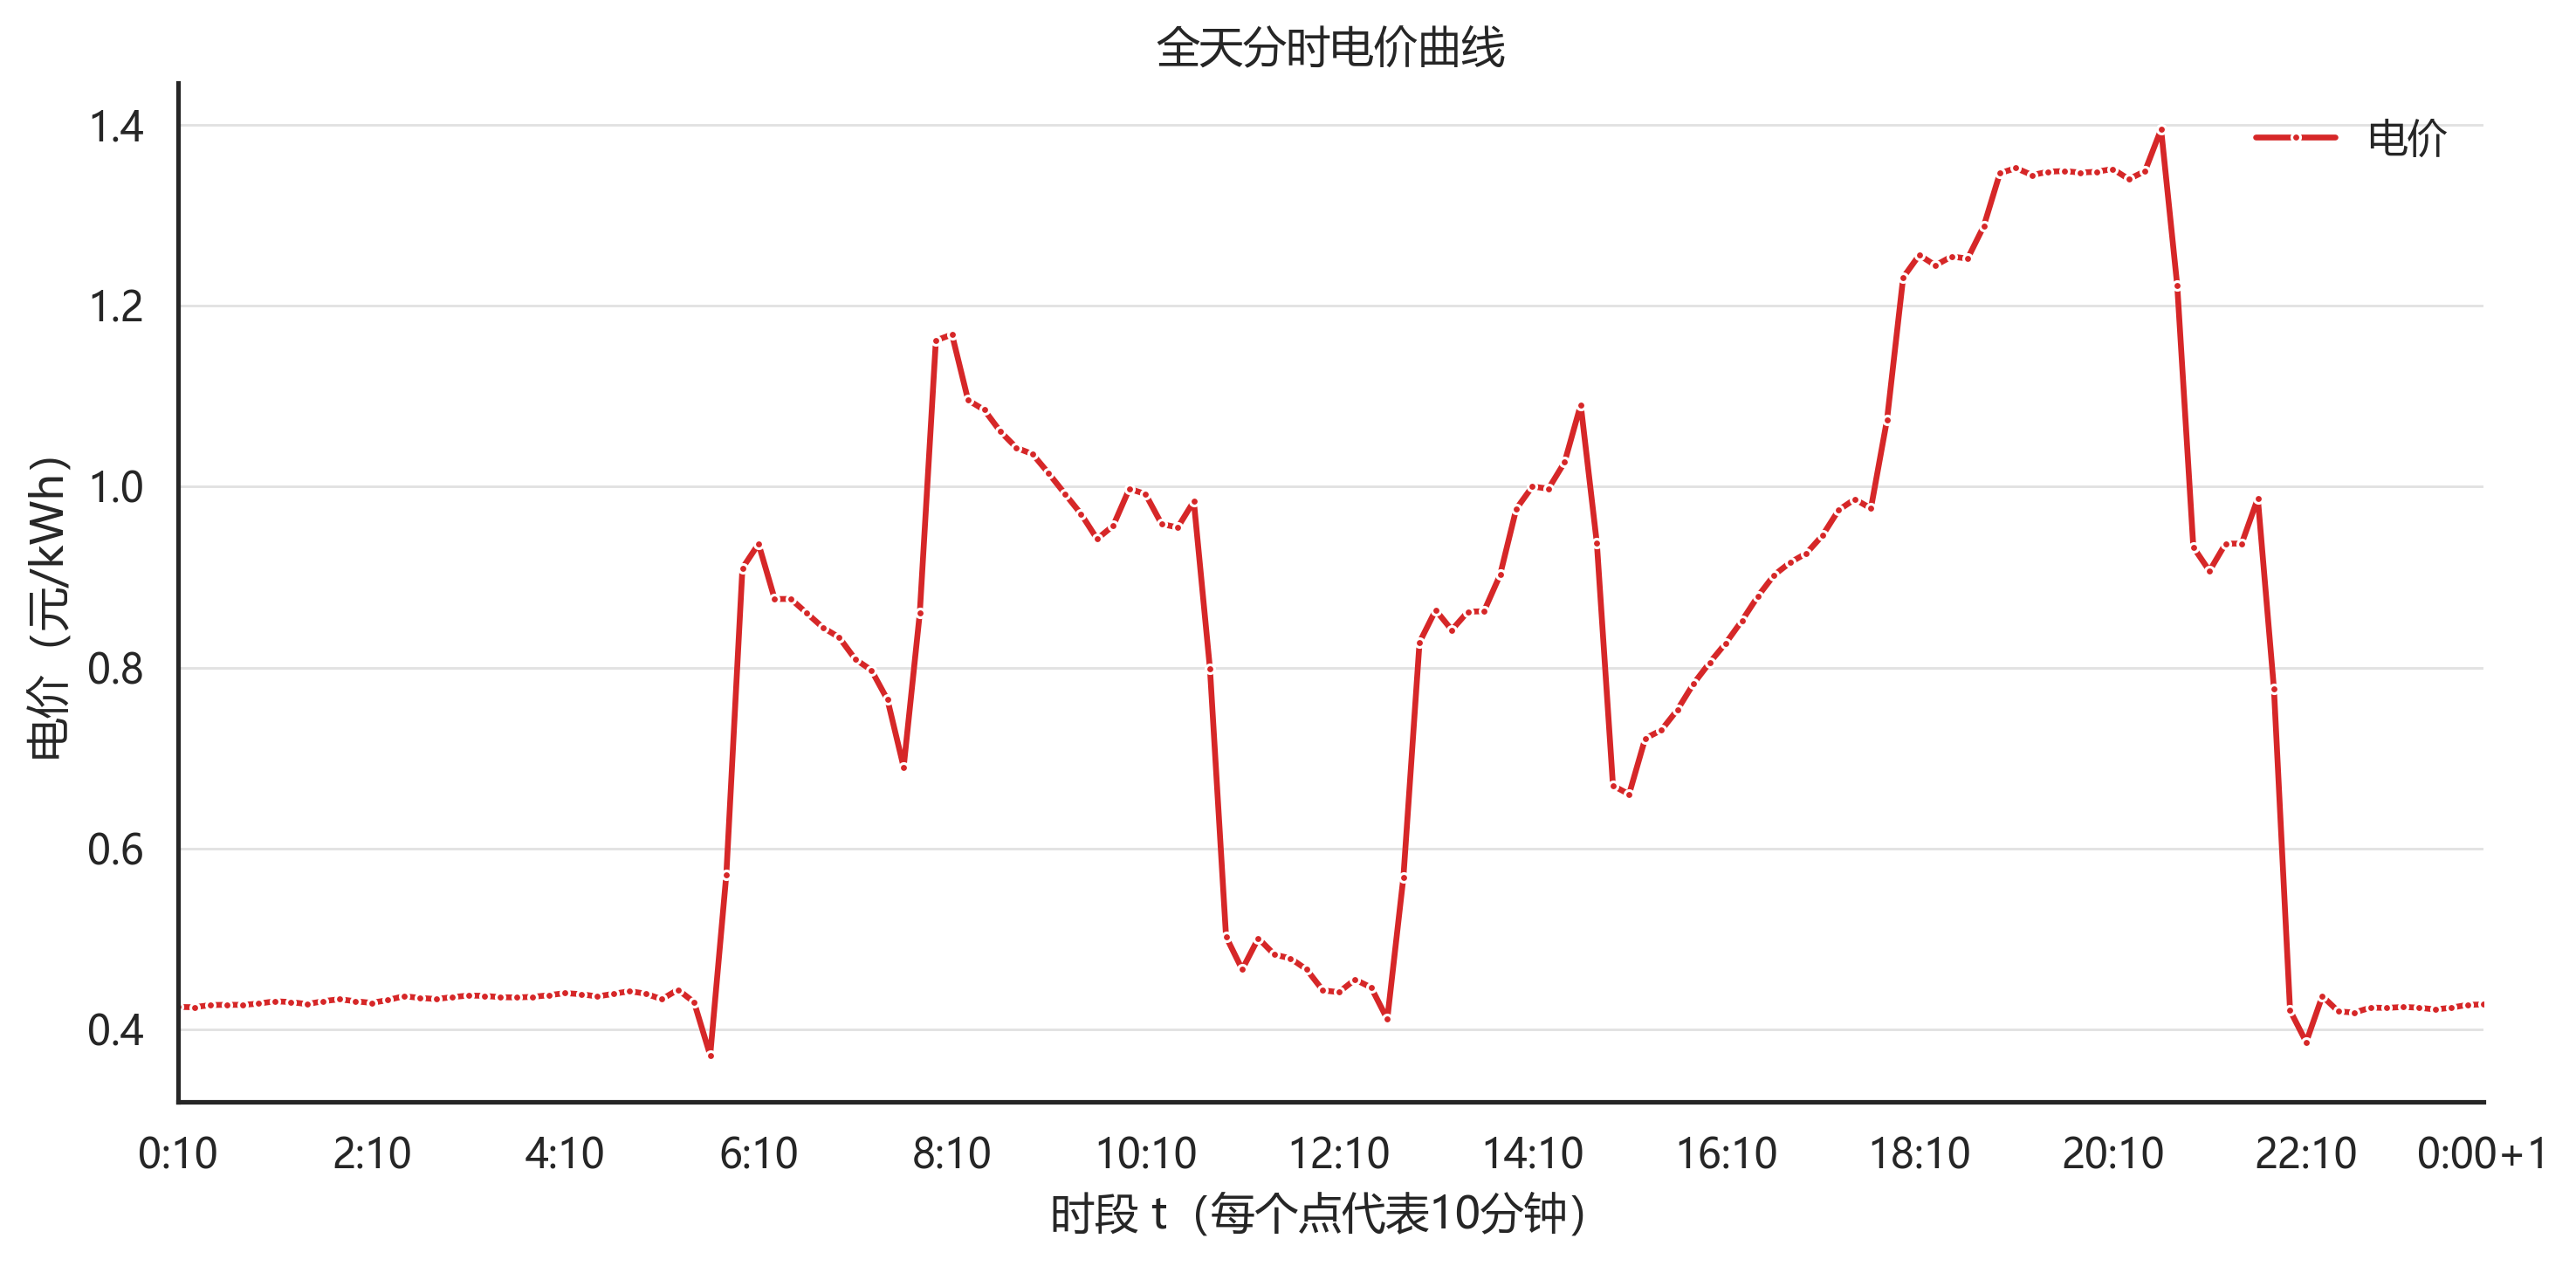
\includegraphics[width=0.33\textwidth]{./figures/图1.png}}
    \subfloat[全天负载与光伏预测功率曲线]
    {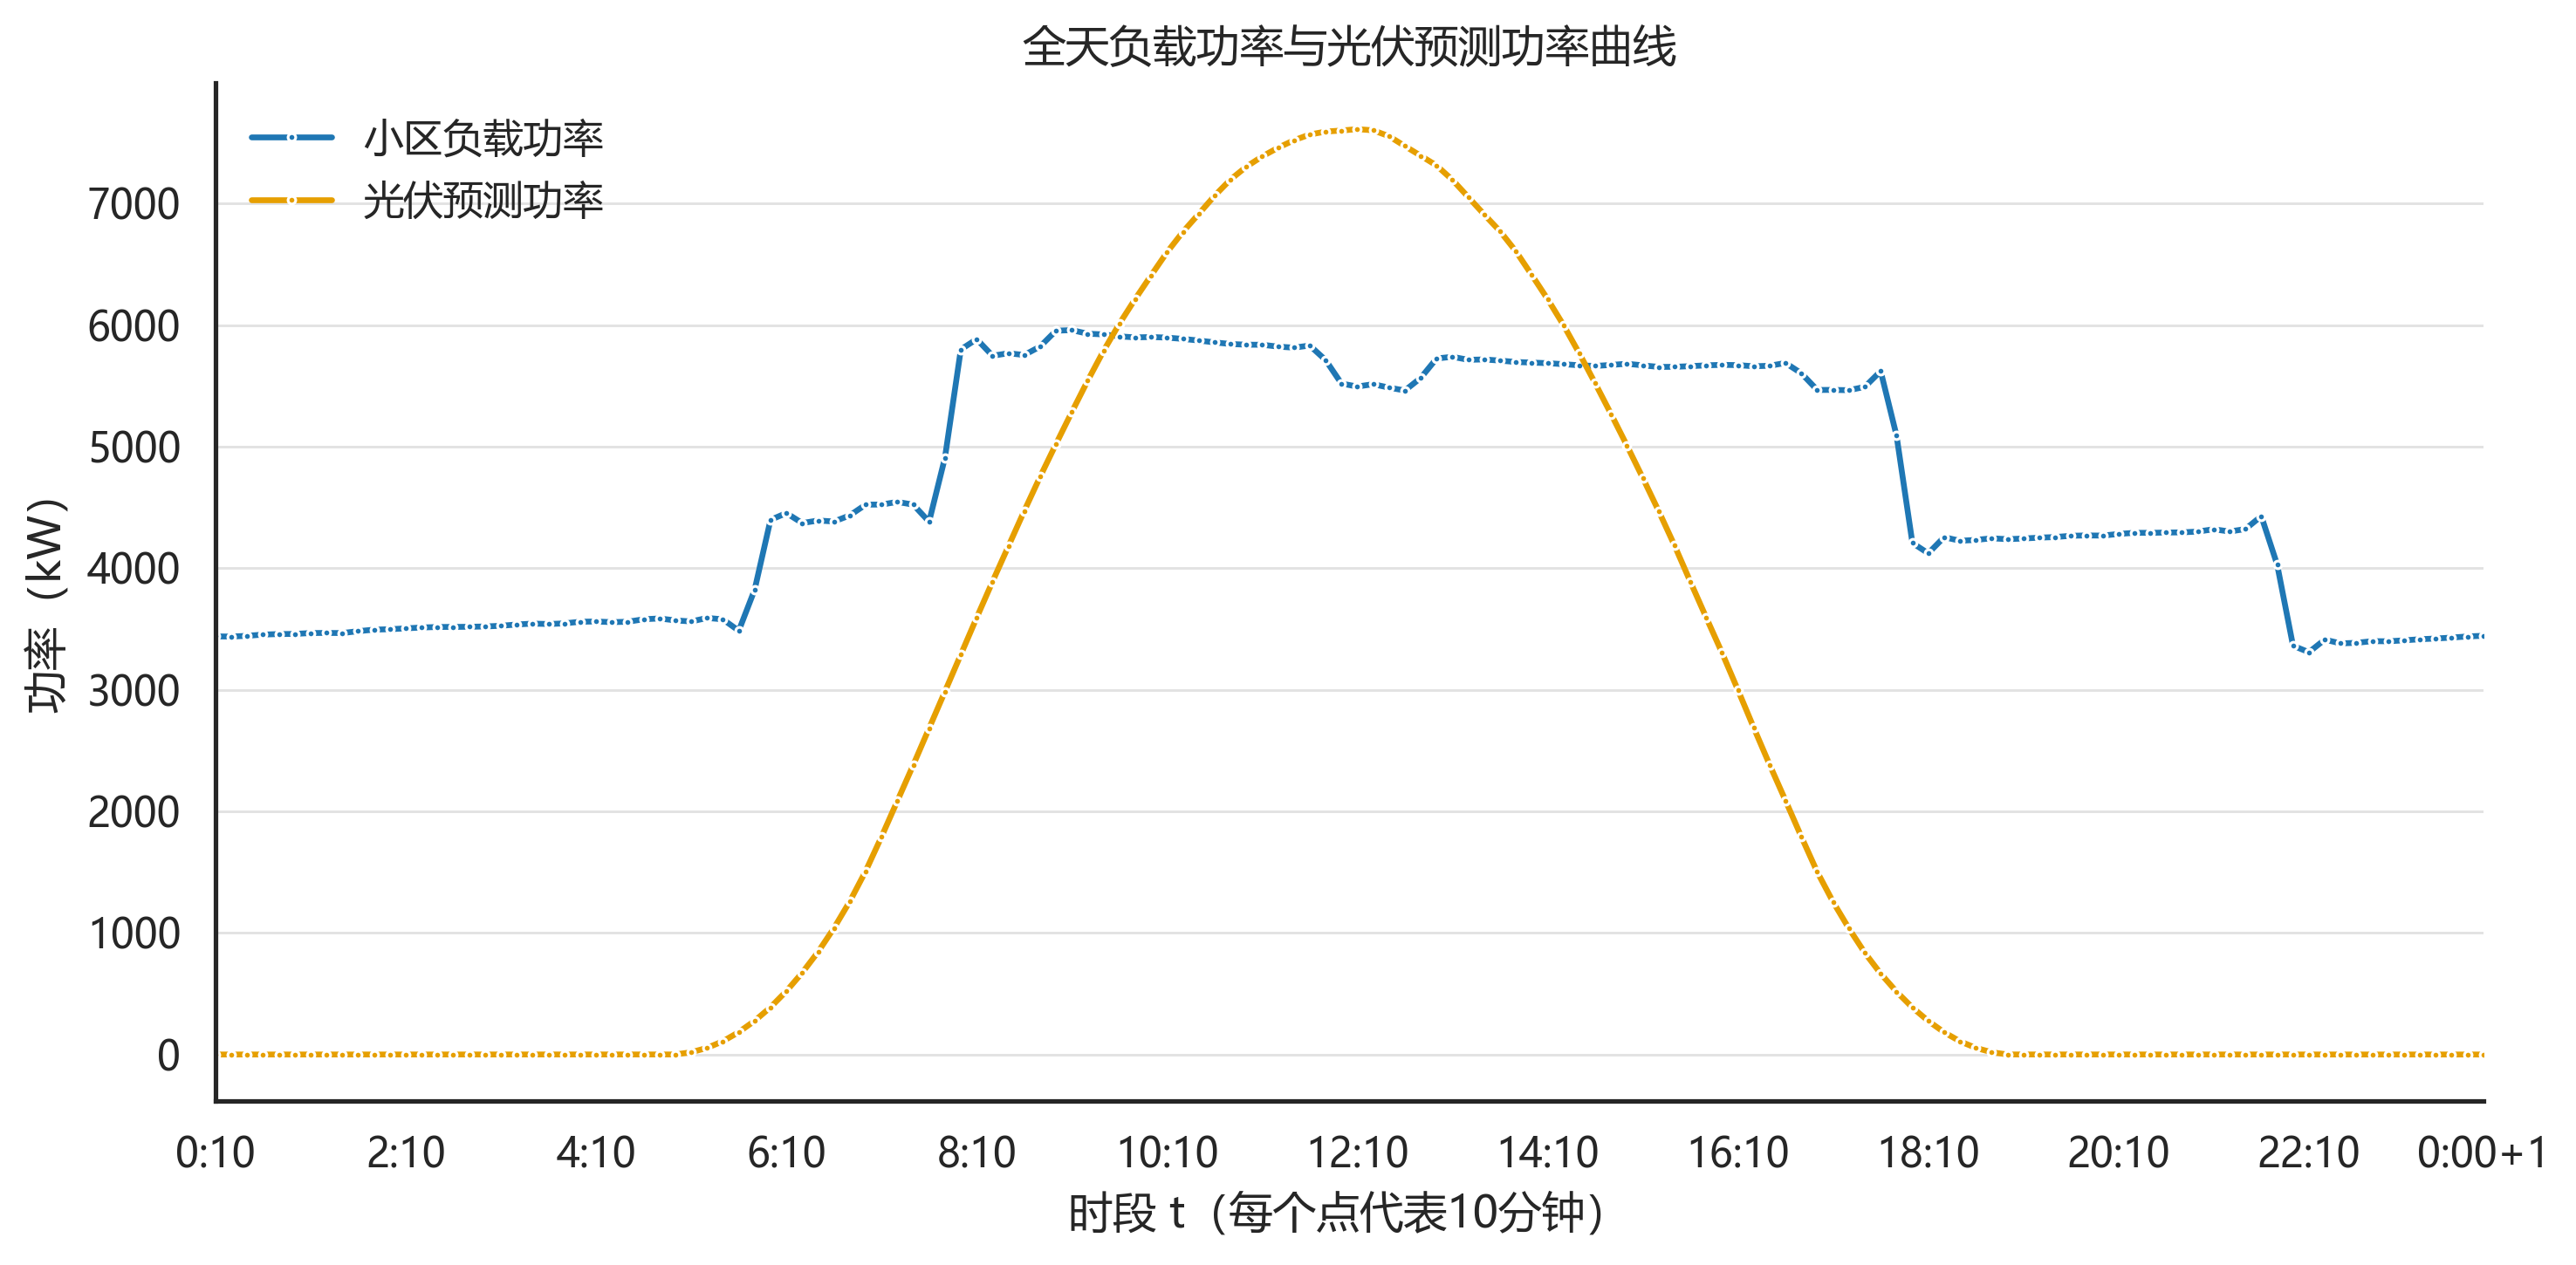
\includegraphics[width=0.33\textwidth]{./figures/图2.png}}
    \subfloat[全天净负载功率曲线]{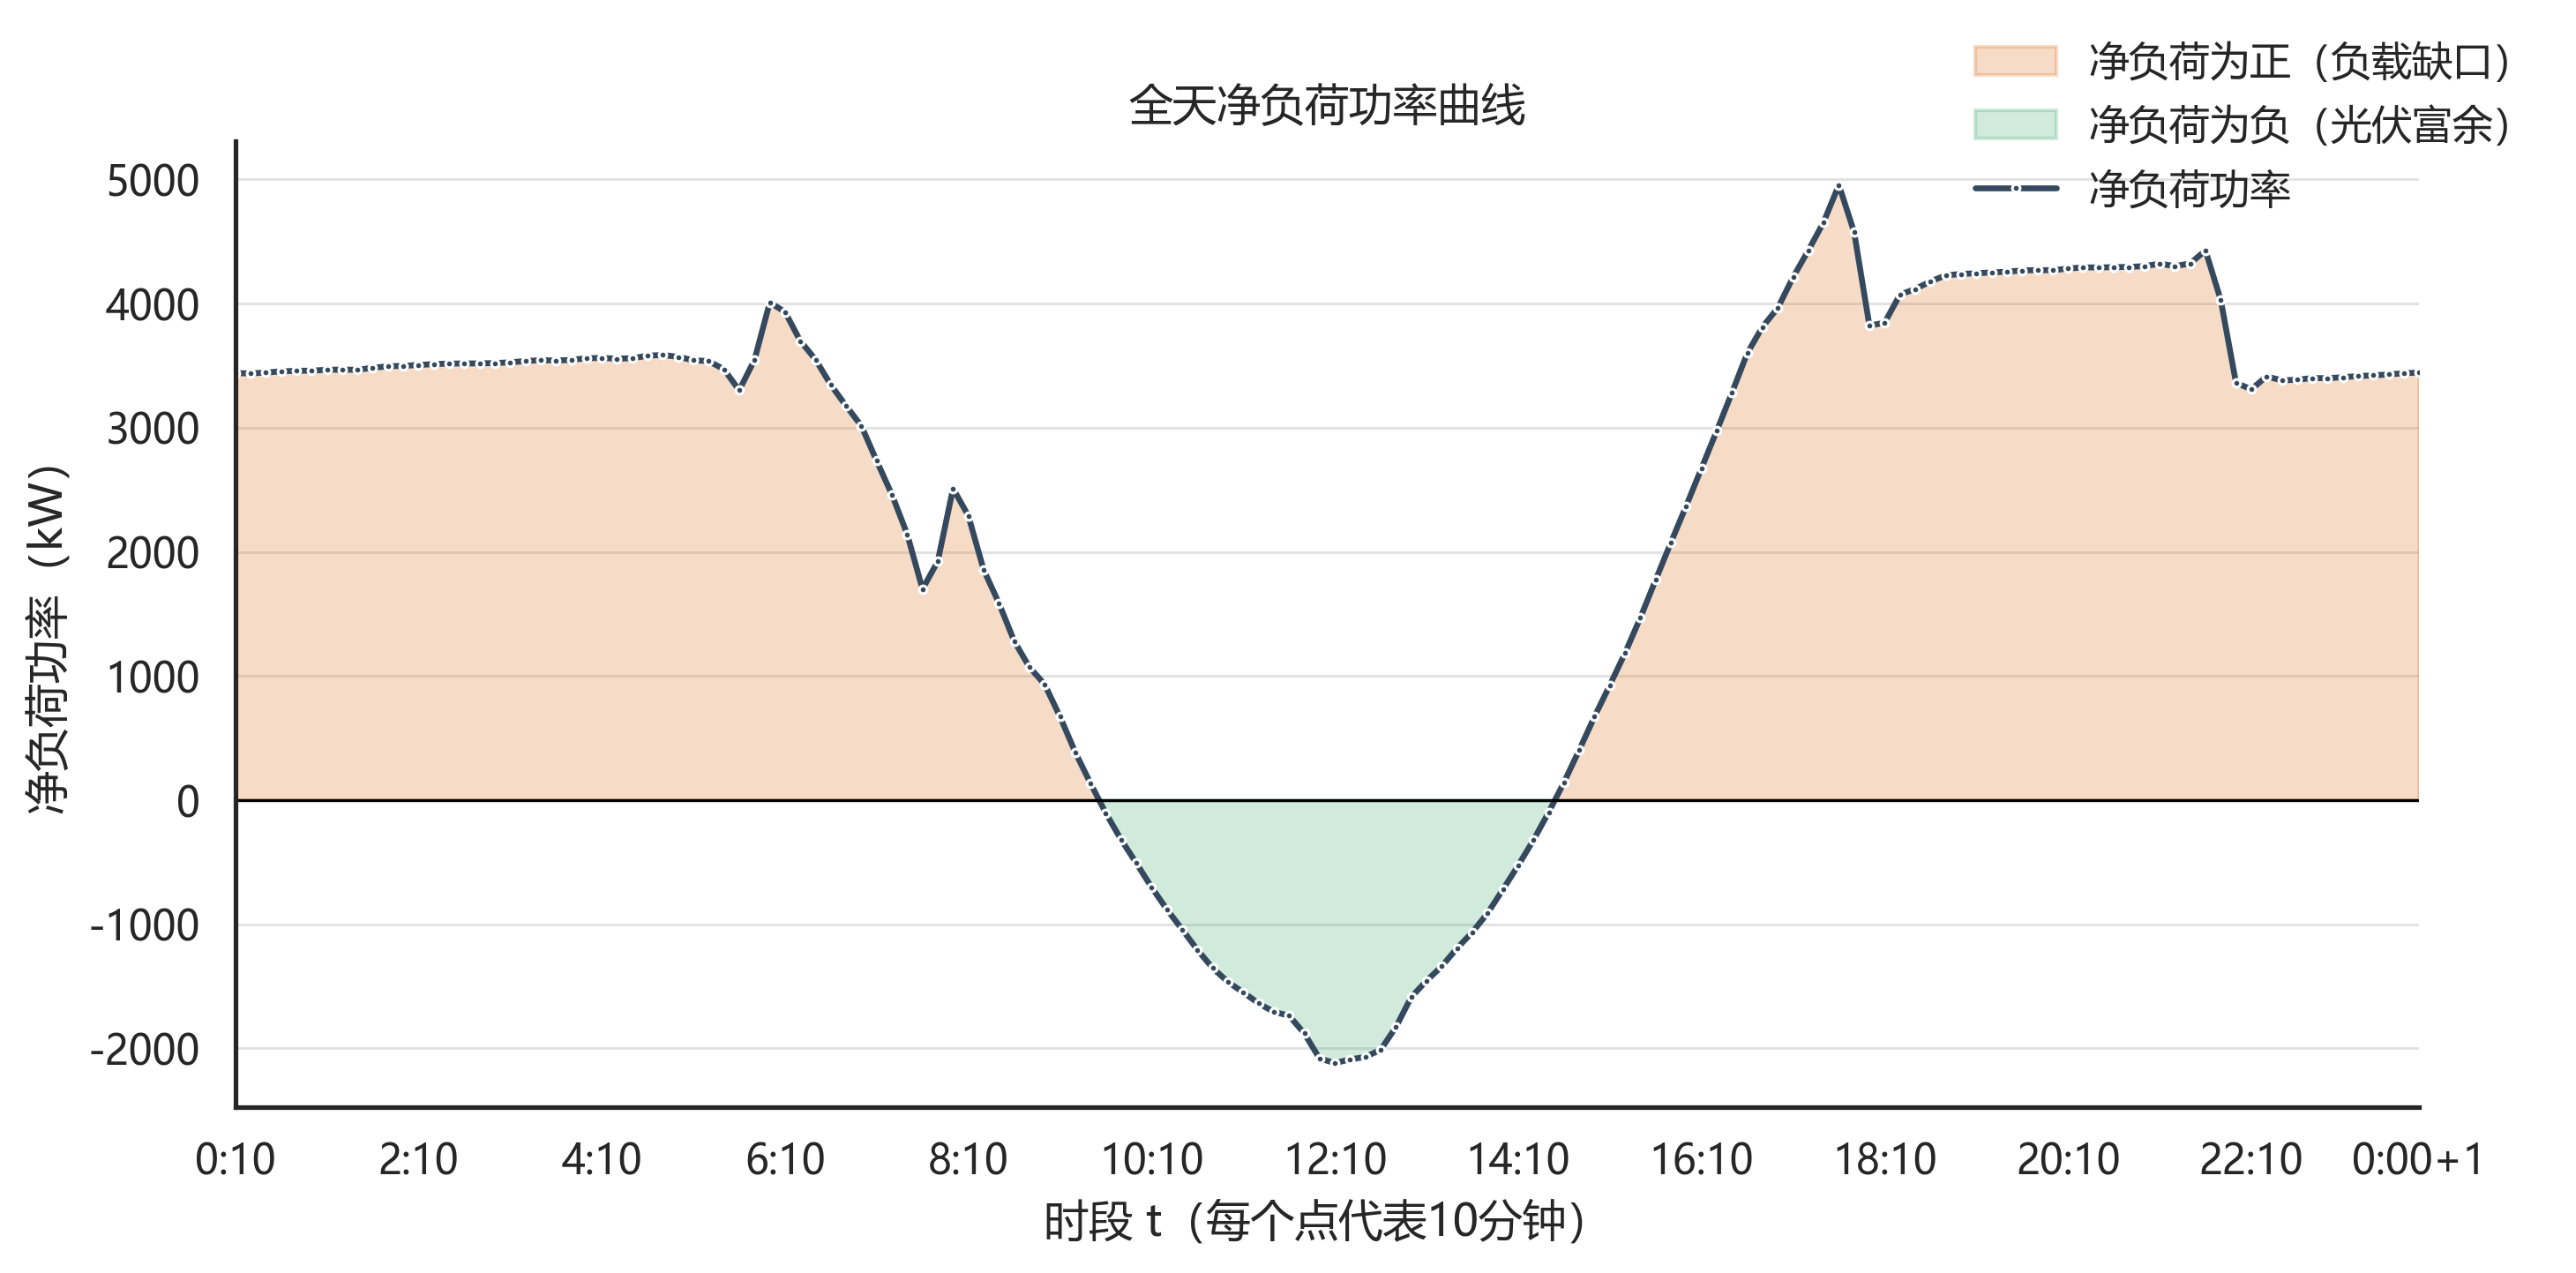
\includegraphics[width=0.33\textwidth]{./figures/图3.png}}
    \caption{全天分时电价、负荷、光伏预测功率及净负载功率曲线}
    \label{fig:q1_1}
\end{figure}


\noindent
\begin{minipage}[t]{0.31\textwidth}
\small
\end{minipage}
\hfill
\begin{minipage}[t]{0.31\textwidth}
\small
\end{minipage}
\hfill
\begin{minipage}[t]{0.31\textwidth}
\small
\end{minipage}

\vspace{0.5em}
由图 \ref{fig:q1_1}（a） 可知，凌晨 0:10--5:50 电价维持在 0.4 元/kWh 左右低谷；6:00 后快速攀升，上午 8:00 左右出现第一个峰值（约 1.17 元/kWh）；10:00--12:00 回落至 0.4--0.5 元/kWh ，为午间低谷，此后开始不规则回升回落（14:00 回升至最高1.09 元/kWh,随后又下降至最低 0.68 元/kWh）；傍晚 17:00--21:00 反升至全天最高（接近 1.40 元/kWh），随后逐渐下降，最终呈现\textbf{不规则双峰结构}。

图 \ref{fig:q1_1} (b)展示供需两侧功率变化。小区负载凌晨维持约 3400 kW，上午 8:00 后上升至 5500--6000 kW 并保持至傍晚，夜间回落至 3300 kW 左右；光伏发电明显符合日光光照情况，夜间为 0，早晨 6:00 后上升，中午 11:00--13:00 达到峰值（超过 7000 kW），下午逐渐下降，18:00 后为 0。

净负荷功率情况如图 \ref{fig:q1_1}（右）所示。夜间和早晨光伏出力不足，净负荷为正且较大；约 9:00--14:00 光伏出力超过负载，净负荷为负，出现光伏富余，最小净负荷约为 $-2117.53$ kW，对应十分钟电量约为 $-352.92$ kWh；傍晚 17:00--19:00 净负荷达到最大，最大净负荷功率约为 $4956.50$ kW，对应十分钟电量约为 $826.08$ kWh。

综合三图，凌晨和上午电价较低但净负载较高；午间光伏富余时段净负载为负且电价较低；傍晚高峰时段同时出现高净负载和高电价，初步说明若能在午间低价/负净负载时段储能充电，并在傍晚高电价/高净负载时段放电，可有效降低购电总费用。

\subsection{模型建立与求解}

\subsubsection{模型建立}

基于数据及其统计学信息，由于所有输入参数在优化前均已确定，且目标函数与主要约束均为线性，故建立\textbf{确定性线性规划模型}。

\textbf{（1）决策变量}

对每个时段 $t=1,2,\ldots,144$，定义以下决策变量（单位均为 kWh）：
\begin{itemize}
  \item $G_t$：外网购电量；
  \item $C_t$：储能装置充电量；
  \item $D_t$：储能装置放电量；
  \item $W_t$：弃光量；
  \item $S_t$：第 $t$ 个时段初的储能电量（$S_1$ 为 0:00 初值，$S_{145}$ 为 00：00 +1 末值）。
\end{itemize}

其中 $S_t$ 为状态变量，$G_t,C_t,D_t,W_t$ 为控制变量。为消除可能出现的无意义的同时充放电，在目标函数中加入充放电惩罚项。

\textbf{（2）目标函数}

最小化全天外网购电总费用：
\begin{equation}
\min Z=\sum_{t=1}^{144}p_tG_t+\varepsilon\sum_{t=1}^{144}(C_t+D_t),
\label{eq:q1-objective}
\end{equation}
式中 $p_t$ 为第 $t$ 个时段的分时电价（元/kWh），$\varepsilon=10^{-8}$ 为充放电惩罚系数，其值的设定见后文敏感性分析。

\textbf{（3）约束条件}

\quad \textbf{能量平衡约束：} 每个时段内，外网购电、光伏发电与储能放电之和应等于负载、储能充电与弃光之和，即输入与输出平衡：
\begin{equation}
G_t+P_t+D_t=L_t+C_t+W_t,\quad t=1,2,\ldots,144.
\label{eq:q1-balance}
\end{equation}

\quad \textbf{储能状态方程：} 储能电量随时段按充放电效率演化：
\begin{equation}
S_{t+1}=S_t+\eta C_t-\frac{D_t}{\eta},\quad t=1,2,\ldots,144,
\label{eq:q1-soc}
\end{equation}
式中 $\eta=0.90$ 为充放电的单向效率。

\quad \textbf{储能容量约束：} 储能电量需维持在稳定使用区间：
\begin{equation}
1200\leq S_t\leq 10800,\quad t=1,2,\ldots,145.
\label{eq:q1-capacity}
\end{equation}

\quad \textbf{充放电功率约束：} 单时段充放电功率不超过 5000 kW：
\begin{equation}
0\leq C_t\leq 5000\times\Delta t=833.3333,\quad
0\leq D_t\leq 833.3333,\quad t=1,2,\ldots,144.
\label{eq:q1-power}
\end{equation}

\quad \textbf{首尾一致性约束：} 00：00 +1时储能电量需回到初始值：
\begin{equation}
S_1=S_{145}=6000.
\label{eq:q1-terminal}
\end{equation}

\quad \textbf{非负性约束：}
\begin{equation}
G_t\geq 0,\quad C_t\geq 0,\quad D_t\geq 0,\quad W_t\geq 0,\quad t=1,2,\ldots,144.
\label{eq:q1-nonnegative}
\end{equation}


\subsubsection{模型求解}

采用 HiGHS 算法\textsuperscript{[1]}求解对上述线性规划，共有 721 个决策变量和 290 个等式约束。求得全天最优购电费用 \textbf{35126.95 元}。\textbf{问题一表一所要求六个指定时段购电量、购电费用及储能装置充放电量见附录表 \ref{tab:app-q1-plan}和表\ref{tab:app-q1-storage}所示}，其中除总费用单位为“元”以外其余单位均为kWh。

图 \ref{fig:q1-dispatch} 展示了10分钟尺度下优化后外网购电功率、储能充放电功率以及储能电量变化的曲线。

\begin{figure}[H]
  \centering
  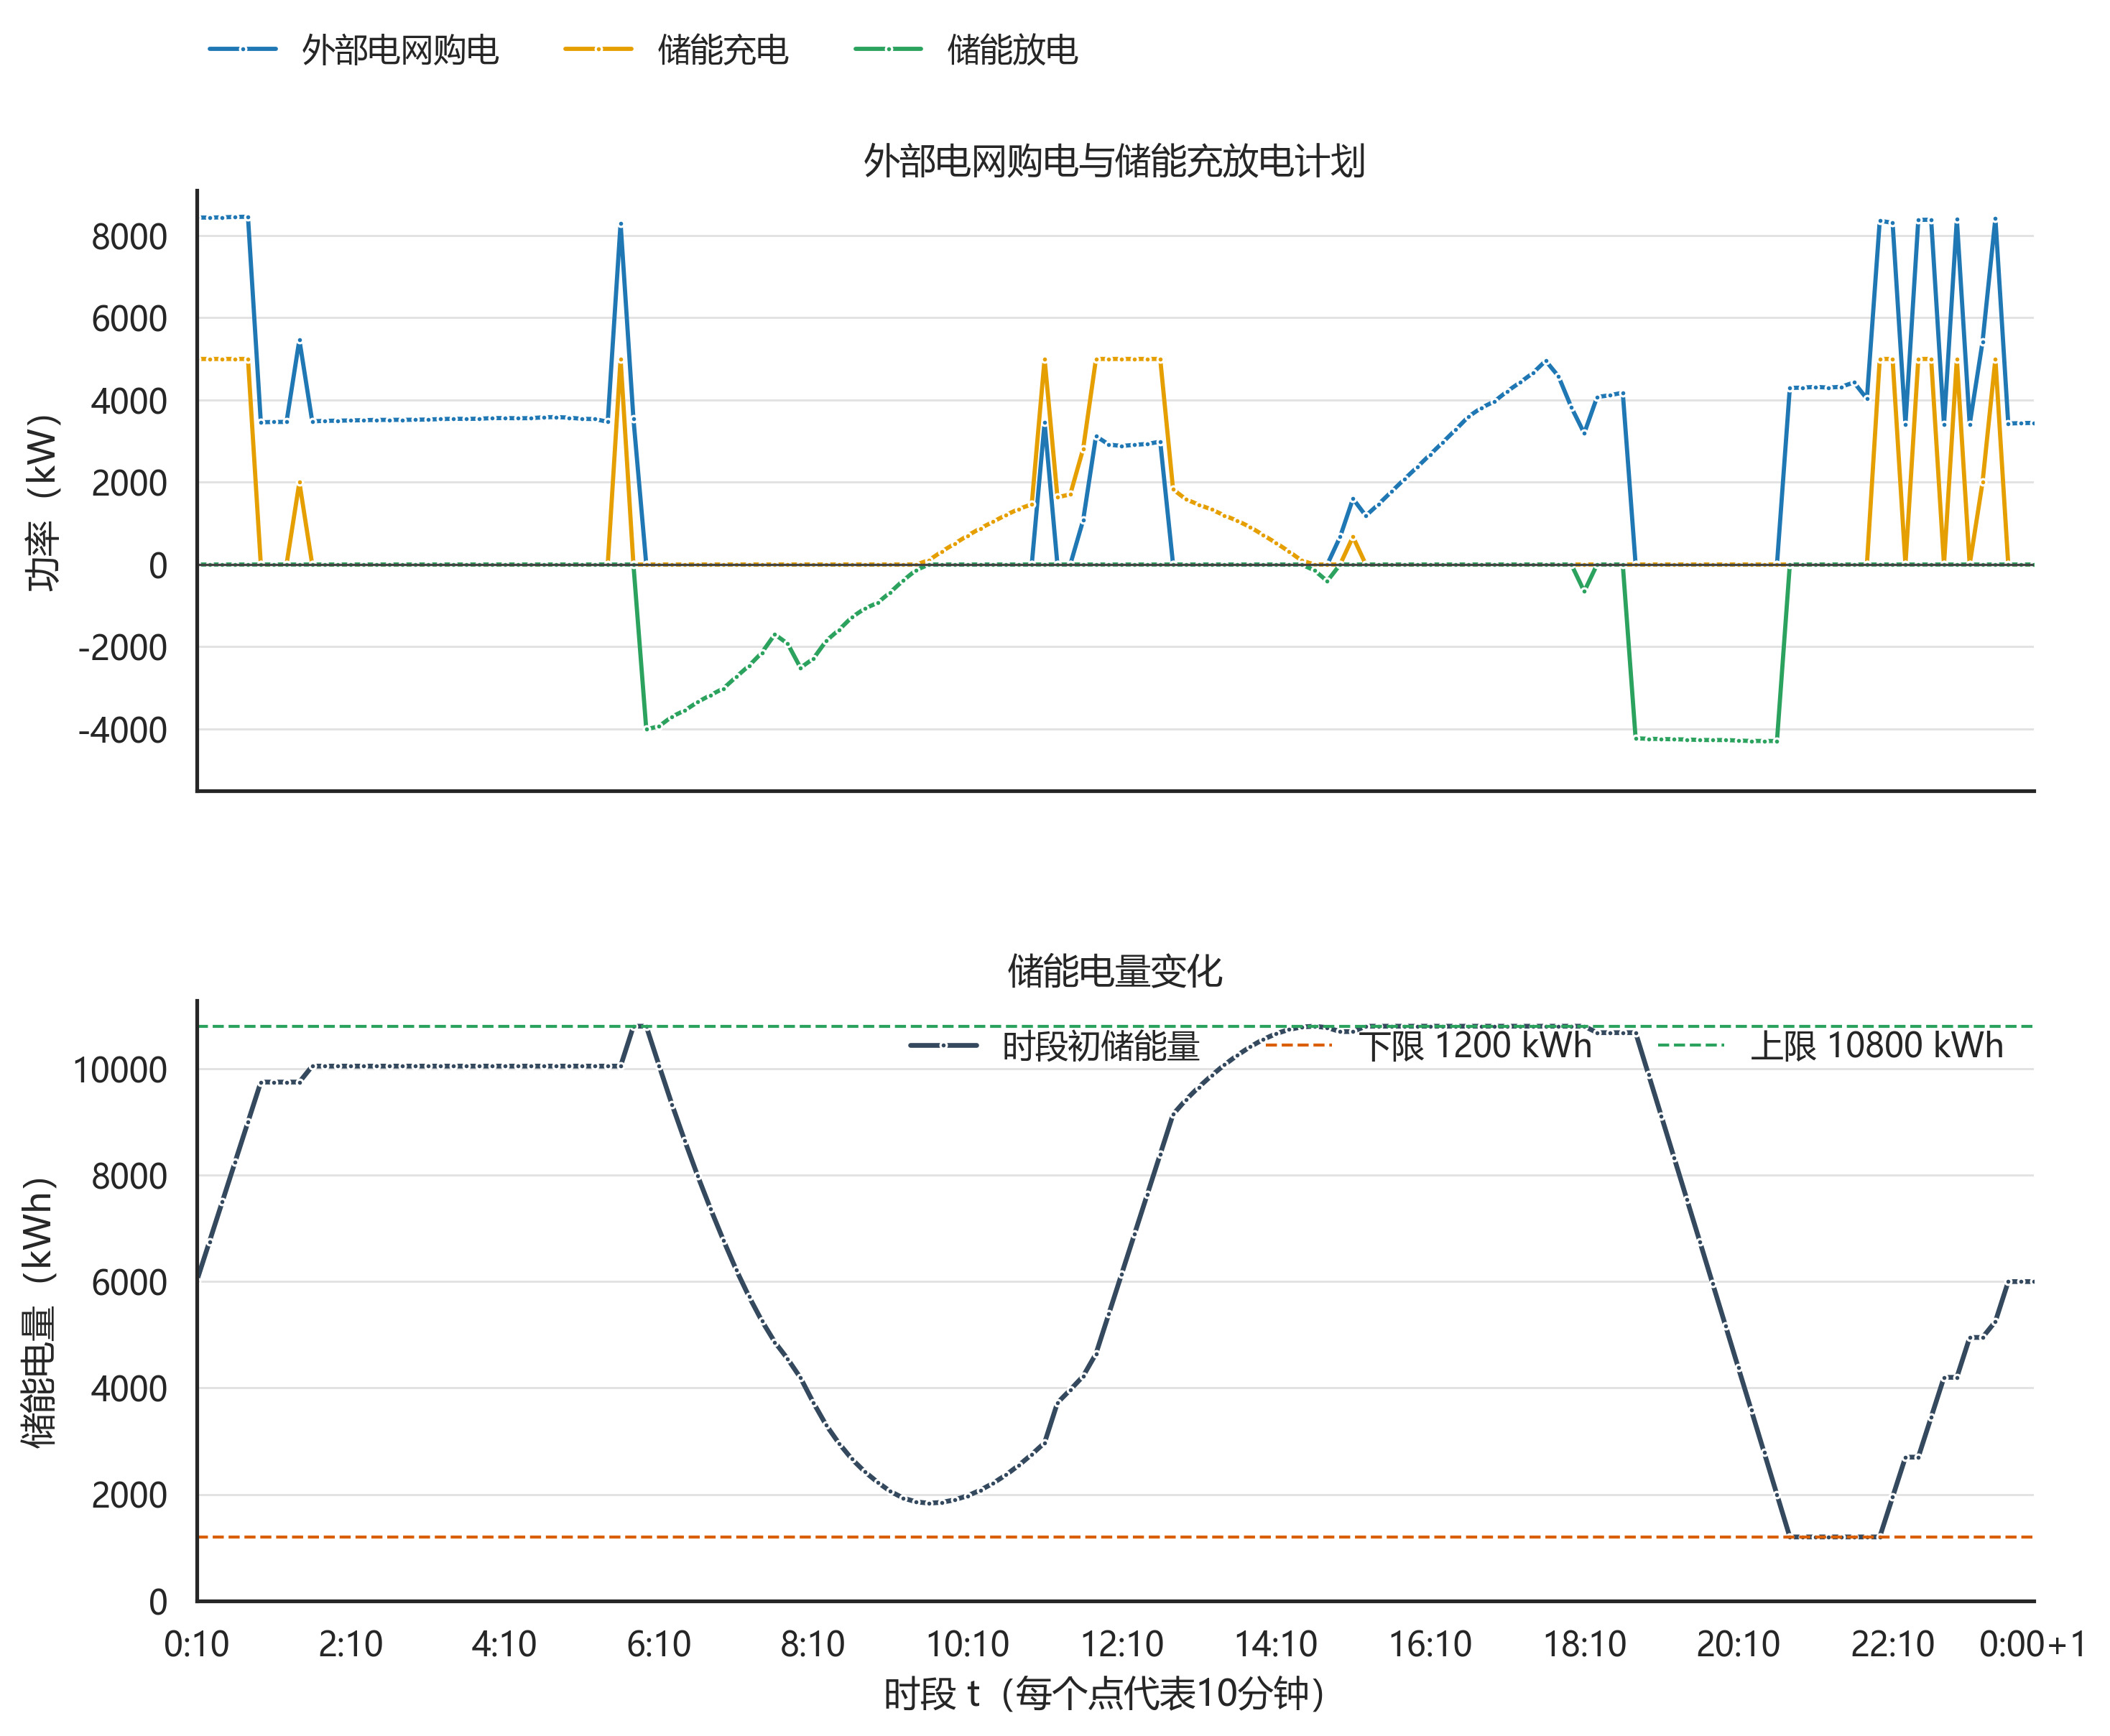
\includegraphics[width=0.95\textwidth]{./figures/图5.png}
  \caption{问题一外网购电、储能充放电与储能电量变化}
  \label{fig:q1-dispatch}
\end{figure}

由图 \ref{fig:q1-dispatch} 可见，凌晨 0:10--5:50 电价处于低谷，优先外网购电并以最大功率向储能充电，储能在约 05:40 首次达到上限 10800 kWh；6:00 后光伏加大效率，但小区负载高速上升，净负载由正转负，储能转为放电以弥补负载缺口；8:00--16:00 光伏功率大幅提高，负载降低后保持较低值且午间电价较低，模型策划此时为储能充电，使储能在 14:30--16:00 期间再次维持在上限附近；傍晚 16:00--21:00 电价与净负载均处高峰，储能持续放电，在约 20:40 达到下限 1200 kWh；夜间 21:00--24:00 电价逐步下降，模型策划重新购电充电，使 00：00 +1时储能回到 6000 kWh，满足首尾一致性约束。在此策略中\textbf{未出现弃光}，说明在现有储能容量与功率约束下，光伏富余电量可被充分利用。

具体购电策略已填入result1.xlsx。

\subsection{光伏预测功率误差分析}

问题一假设典型日的光伏预测功率无偏差，然而实际光伏功率受云层、温度等随机因素影响。现考虑预测误差，对光伏预测功率分别施加系统性比例偏差，重新求解线性规划并统计费用变化。

保持其他参数不变，将附件 1 的光伏预测功率按 $-20\%,-15\%,\ldots,+20\%$ 进行缩放，重新优化得到各情景下的最小购电费用，结果见表 \ref{tab:q1-pv-bias-sensitivity}。

\begin{table}[H]
  \centering
  \caption{光伏预测功率系统性偏差敏感性分析结果}
  \label{tab:q1-pv-bias-sensitivity}
  \small
  \begin{tabularx}{\textwidth}{rrrrrr}
    \toprule
    光伏预测偏差 & 预测电量（kWh） & 购电费用（元） & 相对基准变化（元） & 变化率 & 弃光总量（kWh） \\
    \midrule
    -20\% & 44386.27 & 42269.09 & +7142.14 &+20.33\% & 0.00 \\
    -15\% & 47160.41 & 40294.71 & +5167.76 & +14.71\% & 0.00 \\
    -10\% & 49934.55 & 38422.56 & +3295.61 & +9.38\% & 0.00 \\
    -5\% & 52708.69 & 36697.19 & +1570.24 & +4.47\% & 0.00 \\
    0\% & 55482.84 & 35126.95 & 0.00 & 0.00\% & 0.00 \\
    +5\% & 58256.98 & 33630.58 & -1496.37 & -4.26\% & 0.00 \\
    +10\% & 61031.12 & 32211.93 & -2915.02 & -8.30\% & 0.00 \\
    +15\% & 63805.26 & 31368.20 & -3758.75 & -10.70\% & 1226.62 \\
    +20\% & 66579.40 & 30873.96 & -4252.99 & -12.11\% & 3258.40 \\
    \bottomrule
  \end{tabularx}
\end{table}

由表 \ref{tab:q1-pv-bias-sensitivity} 可知：当光伏预测功率估计偏低时，模型需从外部电网购买更多电力，购电费用显著上升；当光伏预测功率估计偏高，购电费用下降；当偏差超过 $+15\%$ 后，光伏富余电量开始超过储能消纳能力，出现弃光。结果表明，问题一的最优费用对光伏预测功率的系统性偏差较为敏感，预测精度会直接影响费用评估。

充放电惩罚项系数敏感性分析也同时进行，经检验，当 $\varepsilon\leq10^{-2}$ 时，购电费用保持 35126.95 元不变，总费用的增幅完全来自惩罚项本身；当 $\varepsilon$ 达到 $10^{-1}$或者 $1$时，惩罚项开始对购电费用产生实质影响，购电费用上升至 35319.72 元及48052.05元，但储能峰谷套利可能已经被过度惩罚。最终认为选取 $\varepsilon=10^{-8}$ 作为基准足够小以不改变最优解，又足以消除无意义的充放电多解。
\section{问题二：基于 Fourier 岭回归的三日滚动计划购电策略}

\subsubsection{决策层级与信息结构}

问题二为双阶段（日前与日内）随机决策问题：每天 0:00 处于"日前阶段"，决策者只基于历史信息对当日光伏、负载和电价进行预判，在尽量最小化剩余天内总费用的目标确定 144 个计划购电量 $g^P_t$；一旦提交，当天\textbf{不能}修改。进入每个 10 分钟时段，本时段的真实光伏被观测后可在剩余时段优化储能充放电与紧急购电，但\textbf{绝对不可更改购电策略}，且优化充放电及紧急购电策略只执行当前时段决策。

值得注意的是，如果在第一阶段以全年总费用最小为目标进行优化，求解时间\textbf{过长}，不具备工程与模拟效益，但若只聚焦当天总费用，会导致模型更希望把储能用尽，导致模型稳定后下一日初储能接近1200 kWh(即最小储能)，不具备工程意义且明显达不到最小化全年费用的目的，故综合考虑，在每天节点计算接下来连续多日总费用，考虑到选取连续天数不宜过多增加计算量，模型中取连续三天，即\textbf{三日滚动时域}。还需注意未来两日的计划购电量只是辅助变量，不真正提交给电网，次日 0:00 会重新预测、重新优化，这样即使三天后预测存在较大误差，也不会锁定错误决策，保证策略稳健性。

由于考虑真实情况，本文认为\textbf{任何使用未来真实光伏的决策都属于数据泄漏}，预测、场景构造、日前优化和日内执行必须保持严格因果。

本文发现\textbf{"计划购电的低成本但刚性"与"紧急购电的高成本但灵活"之间存在矛盾权衡}：计划购电偏多虽然可覆盖大部分负载缺口、降低紧急购电，但会造成过度弃光，增加计划电费；计划购电偏少则储能可能无法及时补足，导致高价紧急购电；而在此模型中，紧急购电价格是正常电价的 5 倍，模型对计划购电不足的惩罚远大于计划购电偏多的浪费。因此，最优策略会偏保守，\textbf{适度多买计划电}，把尾部紧急购电风险压到足够低。
 
\subsection{数据预处理}

\subsubsection{数据口径}

附件 1 给出全天 144 个 10 分钟时段电价 $p_t$；附件 2 给出光伏与负载的功率曲线。统一采用"功率 $\times 1/6$"将功率（kW）转换为每个 10 分钟时段的电量（kWh）。时间标签采用附件说法："0:10" 对应时段 $0:10$--$0:20$，最后一列对应次日 $0:00$--$0:10$。

问题二使用附件 1 的电价数据和附件 2 的每天负载、实际光伏数据，经数据处理后生成模型输入文件，主要字段含义见表 \ref{tab:q2-fields}。

\begin{table}[H]
  \centering
  \caption{问题二预处理后数据字段说明}
  \label{tab:q2-fields}
  \small
  \begin{tabularx}{\textwidth}{CCCC}
    \toprule
    字段 & 含义 & 单位或范围 & 建模作用 \\
    \midrule
    \texttt{date} & 日期 & $2025\text{-}01\text{-}01\sim2025\text{-}12\text{-}31$ & 时间索引 \\
    \texttt{t} & 时段编号 & $1,\ldots,144$ & 日内时间索引 \\
    \texttt{price} & 分时电价 & 元/kWh & 购电成本目标函数 \\
    \texttt{load\_kw} & 小区负载功率 & kW & 能量平衡输入 \\
    \texttt{pv\_kw} & 实际光伏功率 & kW & 训练 Fourier 模型 \\
    \texttt{load\_kwh} & 十分钟负载电量 & kWh & 能量平衡约束 \\
    \texttt{pv\_kwh} & 十分钟光伏电量 & kWh & 场景输入 \\
    \bottomrule
  \end{tabularx}
\end{table}

\subsection{因果多步光伏预测}

\subsubsection{Fourier 岭回归}

对规划原点 $d$（即每天 0:00），目标日 $d$ 的预测只使用严格早于 $d$ 的实际光伏数据以避免数据泄漏。对每 10 分钟时段 $t$ 分别建立 Fourier 岭回归\textsuperscript{[2]}：
\begin{equation}
    \hat{R}_{d,t} = \beta_{0,t} + \sum_{k=1}^{K}\left(\beta^{\sin}_{k,t}\sin\frac{2\pi kd}{365}+\beta^{\cos}_{k,t}\cos\frac{2\pi kd}{365}\right),
    \label{eq:q2-fourier}
\end{equation}
其中 $d$ 为一年中的日期序号。同一规划原点同时预测 $d, d+1, d+2$ 三天，以确保三日窗口内所有预测均属于同一个 0:00 的信息集，确保不会在预测未来日时引入中间日的新实际光伏。

对应采用岭回归估计。构造设计矩阵 $X$ 与响应矩阵 $Y$：
\[
X=
\begin{bmatrix}
1 & \sin(\theta_1) & \cos(\theta_1) & \cdots & \sin(K\theta_1) & \cos(K\theta_1)\\
1 & \sin(\theta_2) & \cos(\theta_2) & \cdots & \sin(K\theta_2) & \cos(K\theta_2)\\
\vdots & \vdots & \vdots & & \vdots & \vdots\\
1 & \sin(\theta_n) & \cos(\theta_n) & \cdots & \sin(K\theta_n) & \cos(K\theta_n)
\end{bmatrix},
\quad
Y=
\begin{bmatrix}
P_{1,1}^{P} & P_{1,2}^{P} & \cdots & P_{1,144}^{P}\\
P_{2,1}^{P} & P_{2,2}^{P} & \cdots & P_{2,144}^{P}\\
\vdots & \vdots & & \vdots\\
P_{n,1}^{P} & P_{n,2}^{P} & \cdots & P_{n,144}^{P}
\end{bmatrix},
\]
其中 $Y$ 的每一列对应一个十分钟时段。系数矩阵估计为
\begin{equation}
\widehat B=\left(X^{\top}X+\lambda_F D\right)^{-1}X^{\top}Y,
\label{eq:q2-ridge}
\end{equation}
其中 $\lambda_F$ 为 Fourier 回归正则化参数，$D=\operatorname{diag}(0,1,1,\ldots,1)$ 表示不惩罚截距、惩罚三角函数项。由于每天可用于拟合的历史样本有限，而每个时段需估计 $2K+1$ 个参数，普通最小二乘容易因三角函数项之间的近似共线性而出现参数不稳定；岭回归通过对系数施加 $L_2$ 收缩，降低参数方差并抑制过拟合，使外推预测更稳健，尤其适配季节性周期变化的预测光伏功率指标。

\subsubsection{带加权损失的参数选择}

由于光伏高估会触发昂贵的紧急购电，验证损失对高估误差按 5 倍加权：
\begin{equation}
    \mathcal{L}(\hat{R}, R) = \sum_{t}\left[\mathbb{I}(\hat{R}_t>R_t)(R_t-\hat{R}_t)^2\cdot 5 + \mathbb{I}(\hat{R}_t\le R_t)(R_t-\hat{R}_t)^2\right].
    \label{eq:q2-loss}
\end{equation}
候选参数为谐波阶数 $K\in\{1,2,3,4\}$、岭参数 $\lambda\in\{0.1,1,10,100\}$，通过最近最多 30 天的因果滚动验证选择使加权损失最小的 $(K, \lambda)$ 组合。当历史不足 21 天时，使用附件 1 的冷启动曲线作为预测，冷启动日期不计入误差场景样本。

\subsubsection{预测方法说明与精度}

本问采用\textbf{因果多步 Fourier 岭回归}，其核心要点如下：
\begin{itemize}
    \item \textbf{严格因果性}：目标日 $d$ 的模型只使用严格早于 $d$ 的历史实际光伏，候选参数 $(K,\lambda_F)$ 也通过历史验证日的滚动误差选择，避免任何数据泄漏；
    \item \textbf{多步同原点}：规划原点 $d$ 同时生成 $d, d+1, d+2$ 三天的预测，确保三日窗口内所有预测属于同一个 0:00 的信息集；
    \item \textbf{加权验证损失}：光伏高估会触发紧急购电，验证损失对高估误差按 5 倍加权，从而优选保守性更好的参数；
    \item \textbf{冷启动处理}：不足 21 天时，使用附件 1 拟合的冷启动曲线作为预测，且不计入误差场景样本。
\end{itemize}

\subsection{连续三日误差场景}

\subsubsection{历史误差块}

对历史规划原点 $h$，将同一原点生成的未来三日预测与对应实际值拼成连续误差块：
\begin{equation}
    \boldsymbol{\varepsilon}_h = \left(R_h-\hat{R}_{h|h},\; R_{h+1}-\hat{R}_{h+1|h},\; R_{h+2}-\hat{R}_{h+2|h}\right).
    \label{eq:q2-error-block}
\end{equation}
当前原点为 $d$、窗口长度为 $H$ 时，只使用满足 $h+H\le d$ 的完整历史误差块，从而保证场景构造不引入未来信息。

\subsubsection{场景生成与压缩}

场景光伏通过将误差块叠加到预测曲线上得到：
\begin{equation}
    R_{d+j,t}^{\omega} = \max\left(0,\; \hat{R}_{d+j,t} + \varepsilon_{h,j,t}\right).
    \label{eq:q2-scenario-pv}
\end{equation}

历史误差块按 Euclidean 范数\textsuperscript{[3]}排序，分为最多 12 组；每组用组内均值曲线代表一个场景，概率按组内样本数占比确定，这种压缩可保持概率质量守恒并将原始数十个误差块降维到可计算场景数。

\subsection{三日联合风险日前 LP}

\subsubsection{决策变量}

设窗口长度 $H=\min(3, \text{剩余天数})$。对每个场景 $\omega$ 分配计划购电和光伏：
\begin{itemize}
    \item $g^P_t$：第一阶段变量，当日 144 个计划购电量，所有场景共享；
    \item $g^L_{t,\omega}, g^C_{t,\omega}, g^0_{t,\omega}$：计划购电分别用于满足负载、给储能充电、弃用的部分；
    \item $r^L_{t,\omega}, r^C_{t,\omega}, w_{t,\omega}$：光伏分别用于满足负载、给储能充电、弃用的部分；
    \item $c_{t,\omega}, d_{t,\omega}$：储能在场景 $\omega$ 下的充电量、放电量；
    \item $e_{t,\omega}$：场景 $\omega$ 下的紧急购电量。
\end{itemize}

\subsubsection{约束条件}

计划购电分配、光伏分配、负载平衡、储能充电约束：

\begin{equation}
	\left\{
	\begin{aligned}
    g^L_{t,\omega}+g^C_{t,\omega}+g^0_{t,\omega} &= g^P_t\\
    r^L_{t,\omega}+r^C_{t,\omega}+w_{t,\omega} &= R_{t,\omega}\\
    g^L_{t,\omega}+r^L_{t,\omega}+d_{t,\omega}+e_{t,\omega} &= L_t\\
    g^C_{t,\omega}+r^C_{t,\omega} &= c_{t,\omega}
	\end{aligned}
	\right.
\end{equation}
\vspace{5pt}

储能状态演化方程：
\begin{equation}
    s_{t+1,\omega} = s_{t,\omega} + 0.9 c_{t,\omega} - \frac{d_{t,\omega}}{0.9}
    \label{eq:q2-soc}
\end{equation}

\subsubsection{目标函数}

目标函数包含计划费用、未来预计费用、紧急购电期望与风险、吞吐量惩罚和终态 SOC 软约束：
\begin{equation}
    \min\; C_{\text{plan}} + E[C_{\text{future}}] + E[C_{\text{emergency}}] + \lambda \cdot \text{CVaR}_{0.90}(C_{\text{emergency}}) + C_{\text{throughput}} + C_{\text{terminal}}
    \label{eq:q2-objective}
\end{equation}

其中风险权重 $\lambda=0.25$（详见后文敏感性分析），CVaR 置信水平为 0.90\textsuperscript{[4]}。三日窗口末不再奖励高 SOC，只惩罚低于窗口初始 SOC 的情况：

\begin{equation}
	\left\{
	\begin{aligned}
    z_\omega &\ge s_{d,0}-s_{d+H,144}\\
    z_\omega &\ge 0
	\end{aligned}
	\right.
\end{equation}
\vspace{5pt}

缺口惩罚系数取平均电价除以效率，表示补回 1 kWh SOC 的近似成本。该设计防止模型为短期费用耗空库存，不鼓励窗口末端人为保留的额外库存。

\subsubsection{滚动执行原则}

未来两日的购电量在三日 LP 中仅为预览变量，不提前写入结果表，不影响次日规划，提交给电网的仅有当日 144 个 $g^P_t$。

\subsubsection{低光伏压力场景}

仅使用历史误差压缩场景时，历史样本可能未覆盖足够低的光伏尾部，导致日前 LP 把所有历史场景的紧急购电压到零，而真实执行仍可能出现缺口。为使 CVaR 具有实际的风险识别能力，在历史场景压缩后增加一个低光伏压力场景：
\begin{itemize}
    \item 压力场景概率取 $1-\alpha=0.10$，与 $\text{CVaR}_{0.90}$ 尾部质量一致；
    \item 有足够历史样本时，按电价加权的光伏短缺风险 $Q_h=\sum_t 5p_t\max(-\varepsilon_{h,t},0)$ 选择最差 10\% 的历史误差块，取其均值作为压力误差场景；
    \item 历史不足时，将点预测整体下调 30\%，即 $R_t^{\text{stress}}=0.7\hat R_t$（作为冷启动压力场景。30\% 的下调幅度参照了鲁棒优化中常用的保守尾部设定，并结合光伏因云层遮挡可能在短时内下降 20\%--40\% 的模拟经验\textsuperscript{[5]}，取中间偏保守值以覆盖典型低光伏尾部）；
    \item 其余历史场景概率按 90\% 等比例缩放，保证所有场景概率和为 1。
\end{itemize}

该压力场景不是一个真实发生概率估计，而是一个可解释的保守尾部情景，用于检验日前计划对低光伏风险的承受能力。实际紧急购电仍由因果日内执行结果确定。

\subsubsection{场景树非预见性约束}
若日前 LP 中每个场景都拥有独立的储能再决策变量，则在优化时相当于已知场景未来的完整光伏路径，违背"未来光伏尚未知晓"的现实。场景树非预见性约束要求在相同历史观测下无法区分的场景必须共享储能和紧急购电决策。

两个场景在时段 $t$ 前（含当前已揭示的光伏）仍无法区分时，要求共享储能和紧急购电决策：

\begin{equation}
	\left\{
	\begin{aligned}
    c_{t,\omega_1}=c_{t,\omega_2}\\
    d_{t,\omega_1}=d_{t,\omega_2}\\
    e_{t,\omega_1}=e_{t,\omega_2}
	\end{aligned}
	\right.
\end{equation}
\vspace{5pt}



未来两日的预览购电在下一日 0:00 才能重新决定，因此只根据此前完整日期的观测历史分组。加入该约束后，日前 LP 不再允许每个场景独立使用未来完整光伏路径进行储能再决策。

\subsection{日内因果滚动执行}

计划购电量锁定后，每 10 分钟时段重新求解剩余时间窗口 LP。未来时段预测由历史误差场景按当前观测软加权得到。每次执行当前 10 分钟充电、放电和紧急购电后进入下一时段求解。

日内供需平衡为：
\begin{equation}
    g^P_t + R_t + d_t + e_t = L_t + c_t + w_t.
    \label{eq:q2-realtime-balance}
\end{equation}

程序按"计划购电 + 当前光伏"是否覆盖负载设置上界：基础供给有余时绝对禁止紧急购电，不足时绝对禁止充电；同时加入 $c_t+d_t\le 5000/6$ 和微小吞吐量费用。这样紧急购电不能给储能充电且无无意义的同时充放电。

\subsection{模型求解与结果分析}

\subsubsection{全年结果}

在完整项目数据上运行上述三日滚动框架，得到 2025 年 2 月 1 日至 12 月 31 日共 334 天的调度结果，如表 \ref{tab:q2-annual-summary} 所示。

\begin{table}[H]
  \centering
  \caption{问题二全年运行结果}
  \label{tab:q2-annual-summary}
  \small
  \begin{tabularx}{\textwidth}{CC}
      \toprule
      指标 & 结果 \\
      \midrule
      计划购电费 & 12,905,515.22 元 \\
      紧急购电费 & 825,521.25 元 \\
      总购电费用 & 13,731,036.47 元 \\
      紧急购电量 & 159,973.16 kWh \\
      发生紧急购电天数 & 229 天 \\
      平均光伏预测 MAE & 31.2120 kWh/10 分钟 \\
      CVaR 高于三日场景期望天数 & 1 天 \\
      1 月 31 日暖机末 SOC & 7,885.95 kWh \\
      \bottomrule
  \end{tabularx}
\end{table}

最终完整结果保存至 result2.xlsx。

\subsubsection{与单日滚动基线对比}

作为对比，单日滚动版本的总费用 15,291,017.18 元、紧急购电量 562,202.32 kWh。三日滚动策略对应总费用下降约 1,559,980.71 元（约 156.00 万元），紧急购电量下降约 402,229.16 kWh（约 40.22 万 kWh）。两者使用相同的因果预测和储能边界，差异主要来自三日 SOC/购电联合规划和软约束策略，说明适度前瞻规划显著降低不确定环境下的购电成本。

\subsubsection{计划购电可视化}

图 \ref{fig:q2-daily-plan-cost}--\ref{fig:q2-plan-vs-price} 给出了基于最终 result2.xlsx 的六组可视化结果。
\begin{figure}[H]
    \centering
    \subfloat[逐日计划购电量与计划购电费]{\label{fig:q2-daily-plan-cost}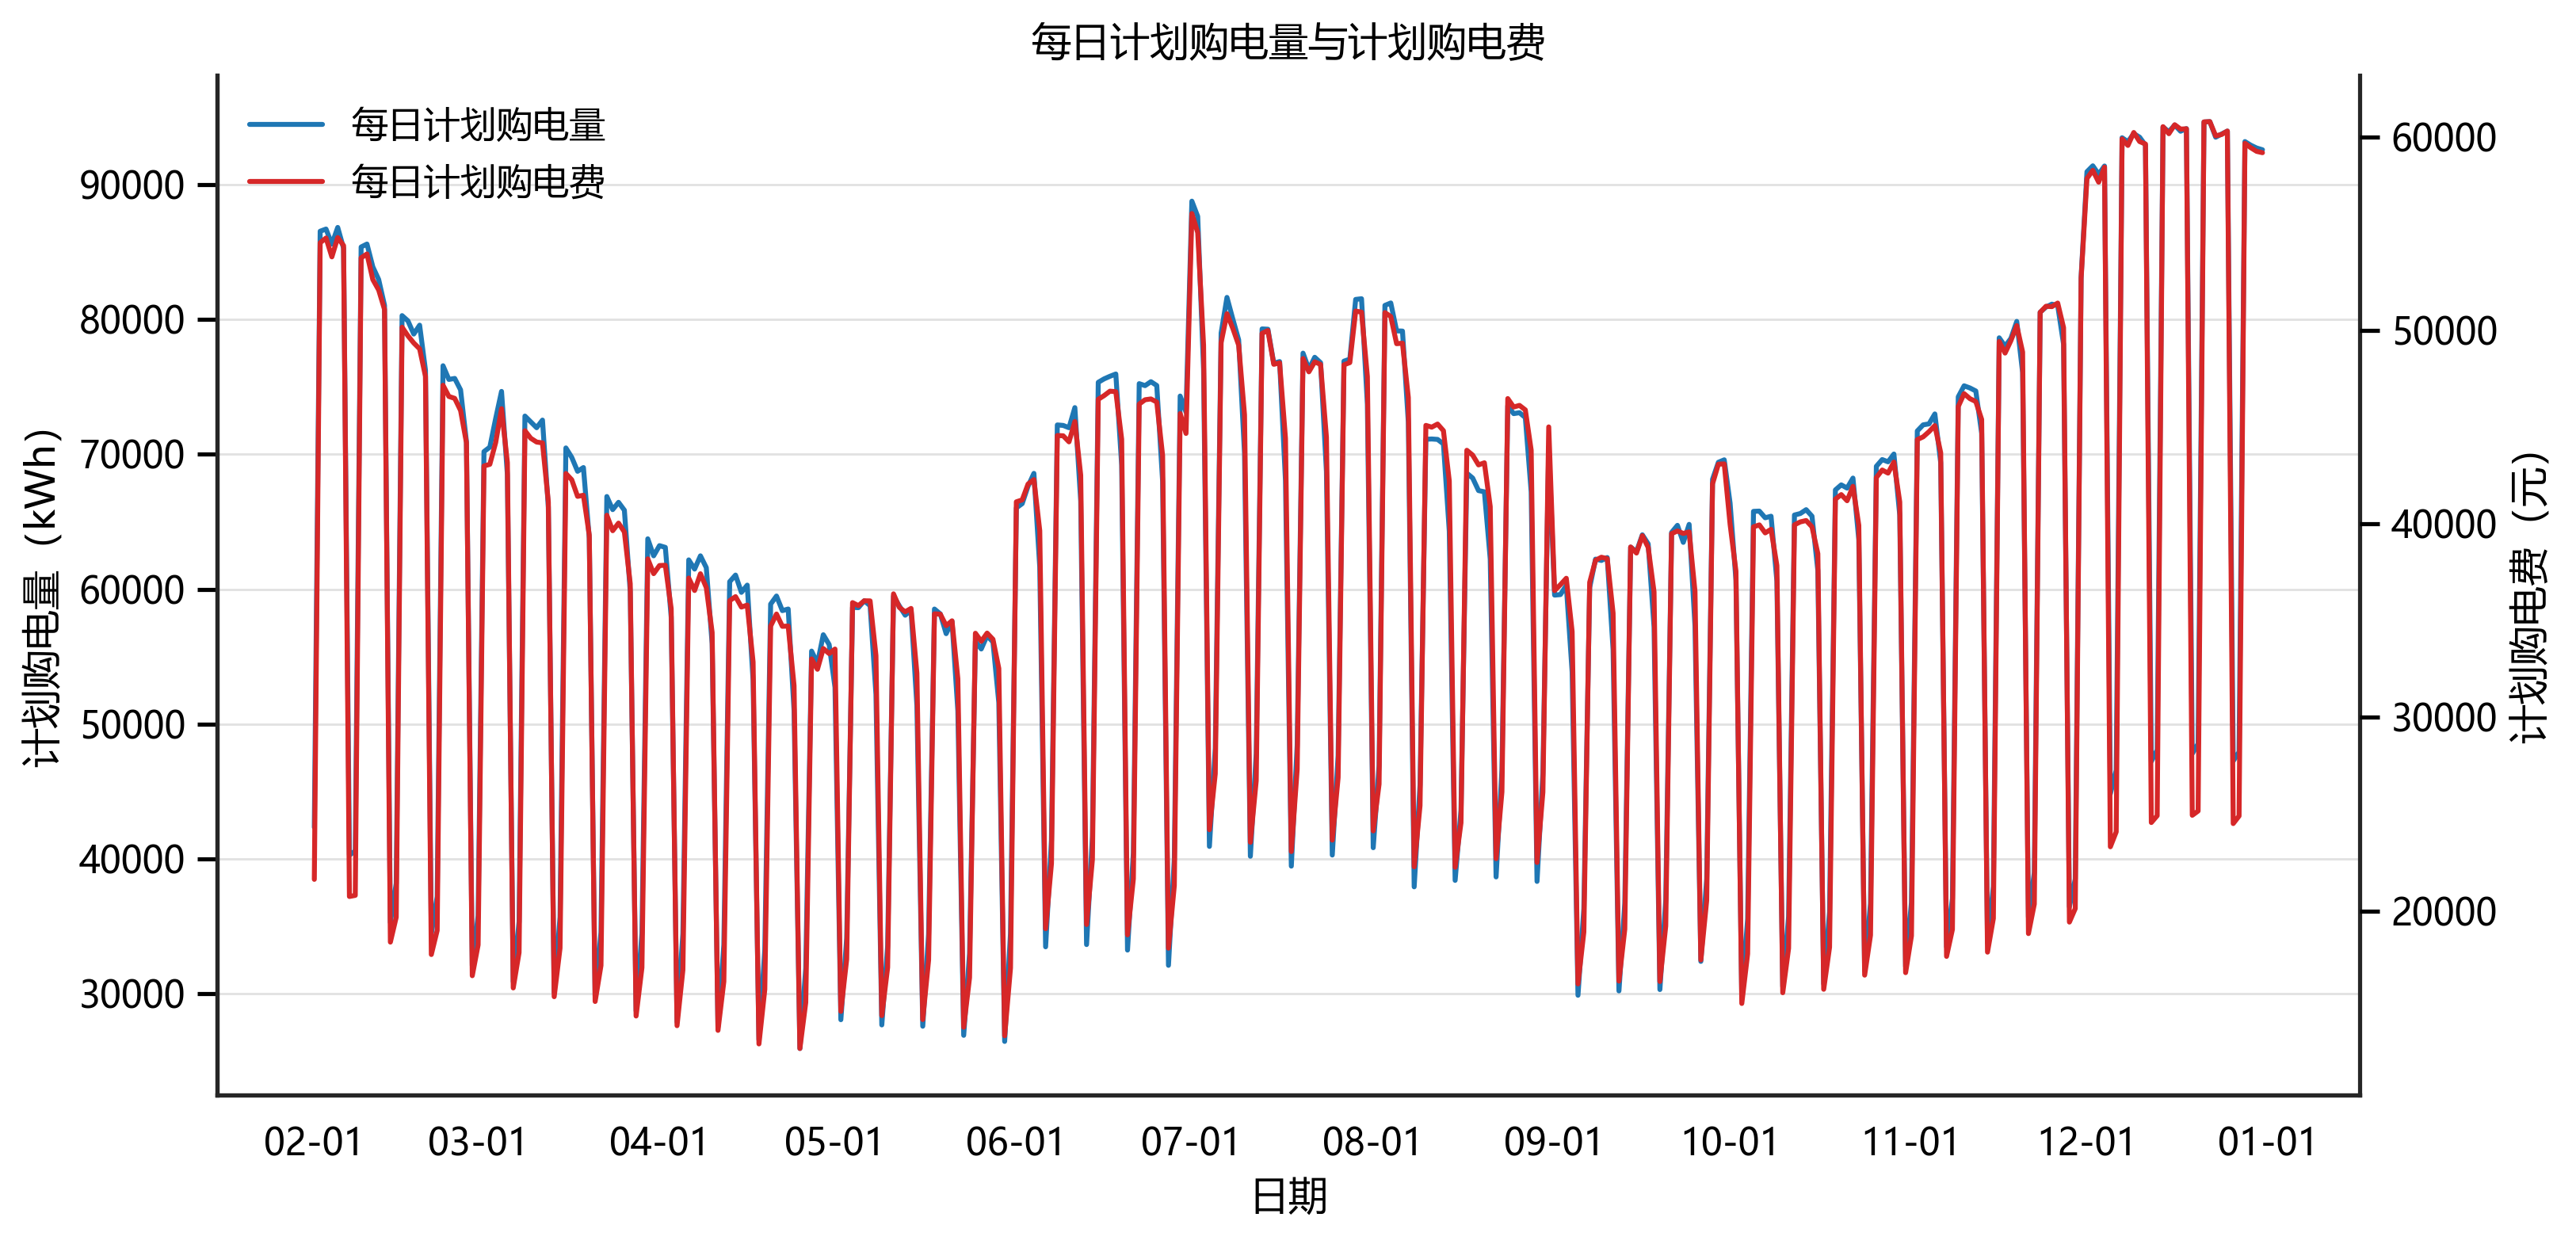
\includegraphics[width=0.49\textwidth]{figures/fig1_daily_plan_purchase_cost.png}}
    \hfill
    \subfloat[全年每天计划购电日历热图]{\label{fig:q2-daily-plan-calendar}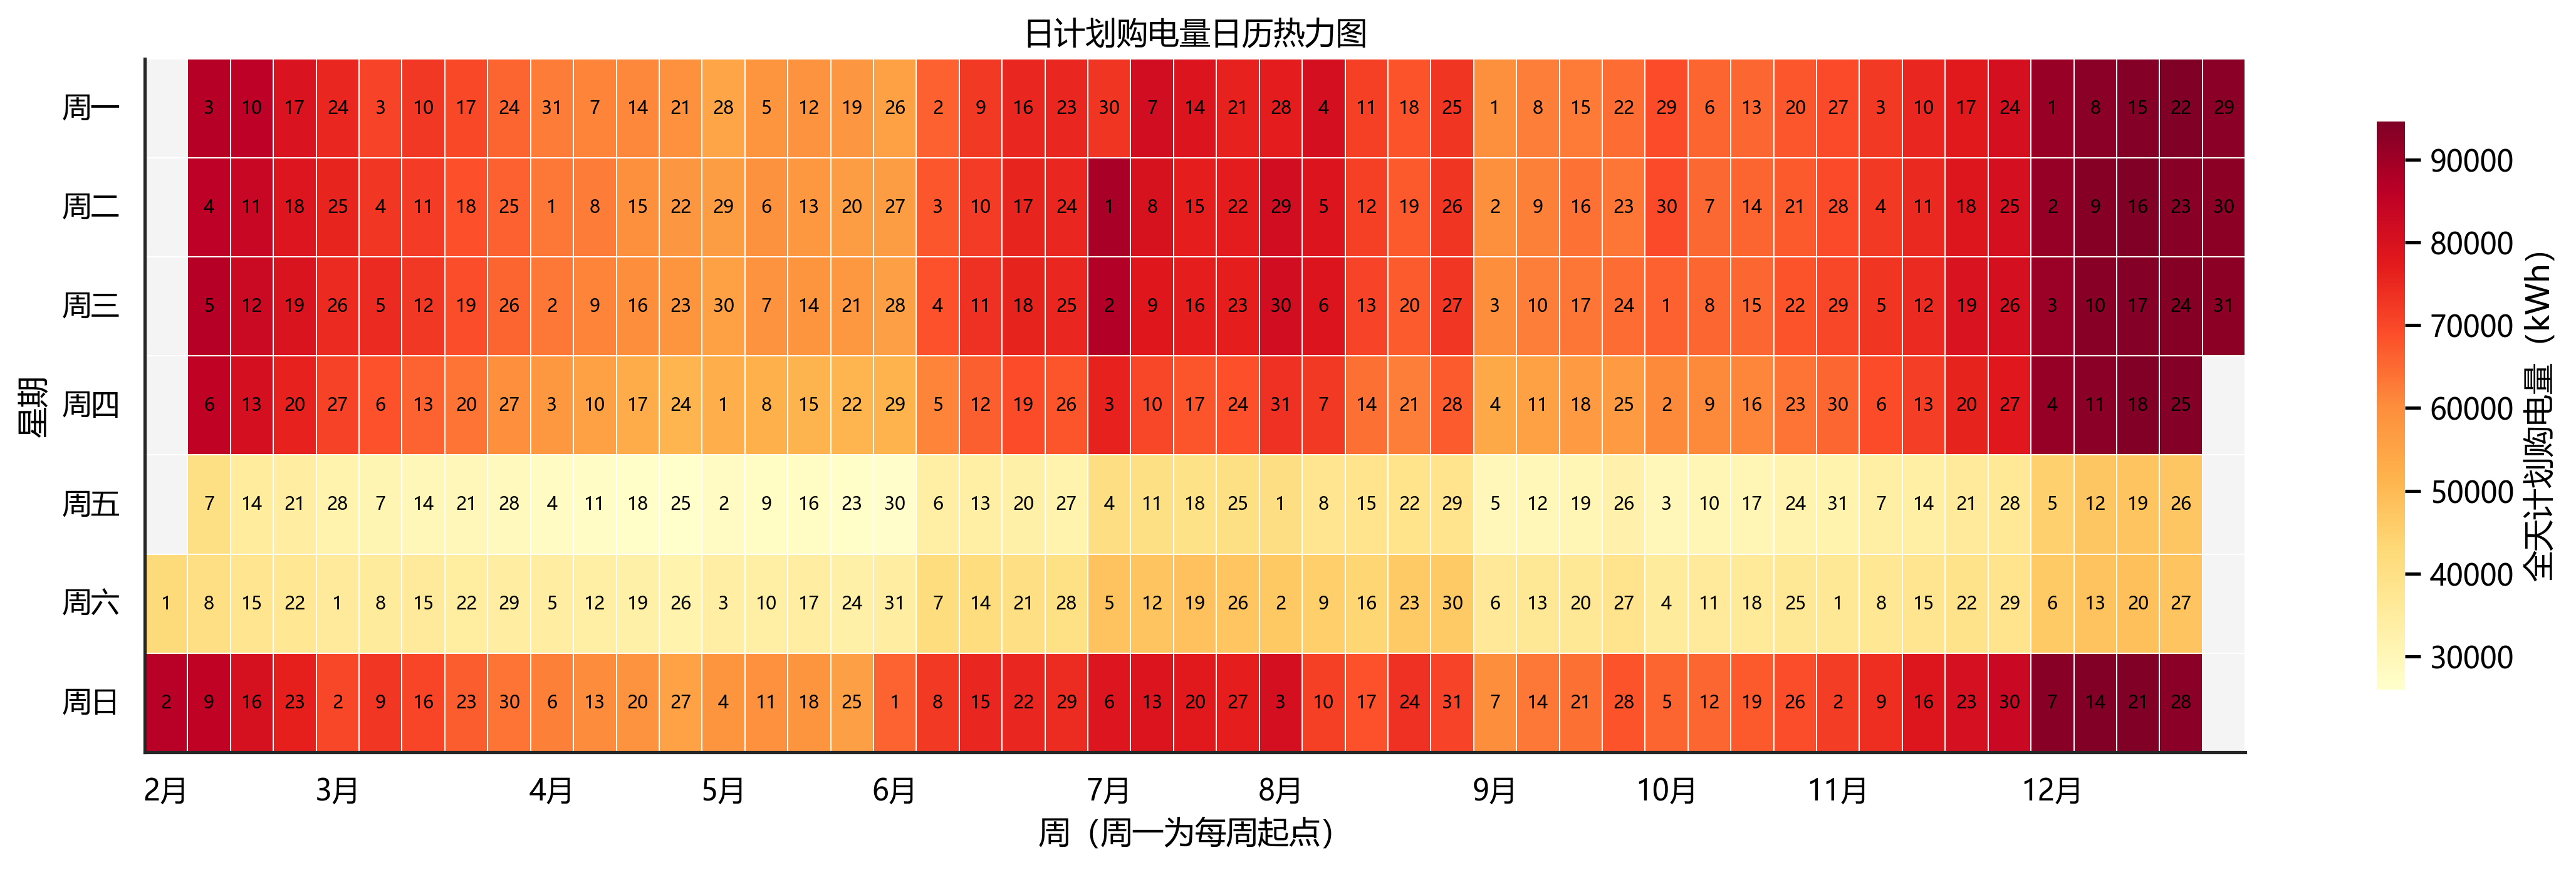
\includegraphics[width=0.49\textwidth]{figures/fig2_daily_plan_calendar.png}}
\end{figure}

\begin{figure}[H]
    \centering
    \subfloat[逐月计划购电量箱线图]{\label{fig:q2-monthly-boxplot}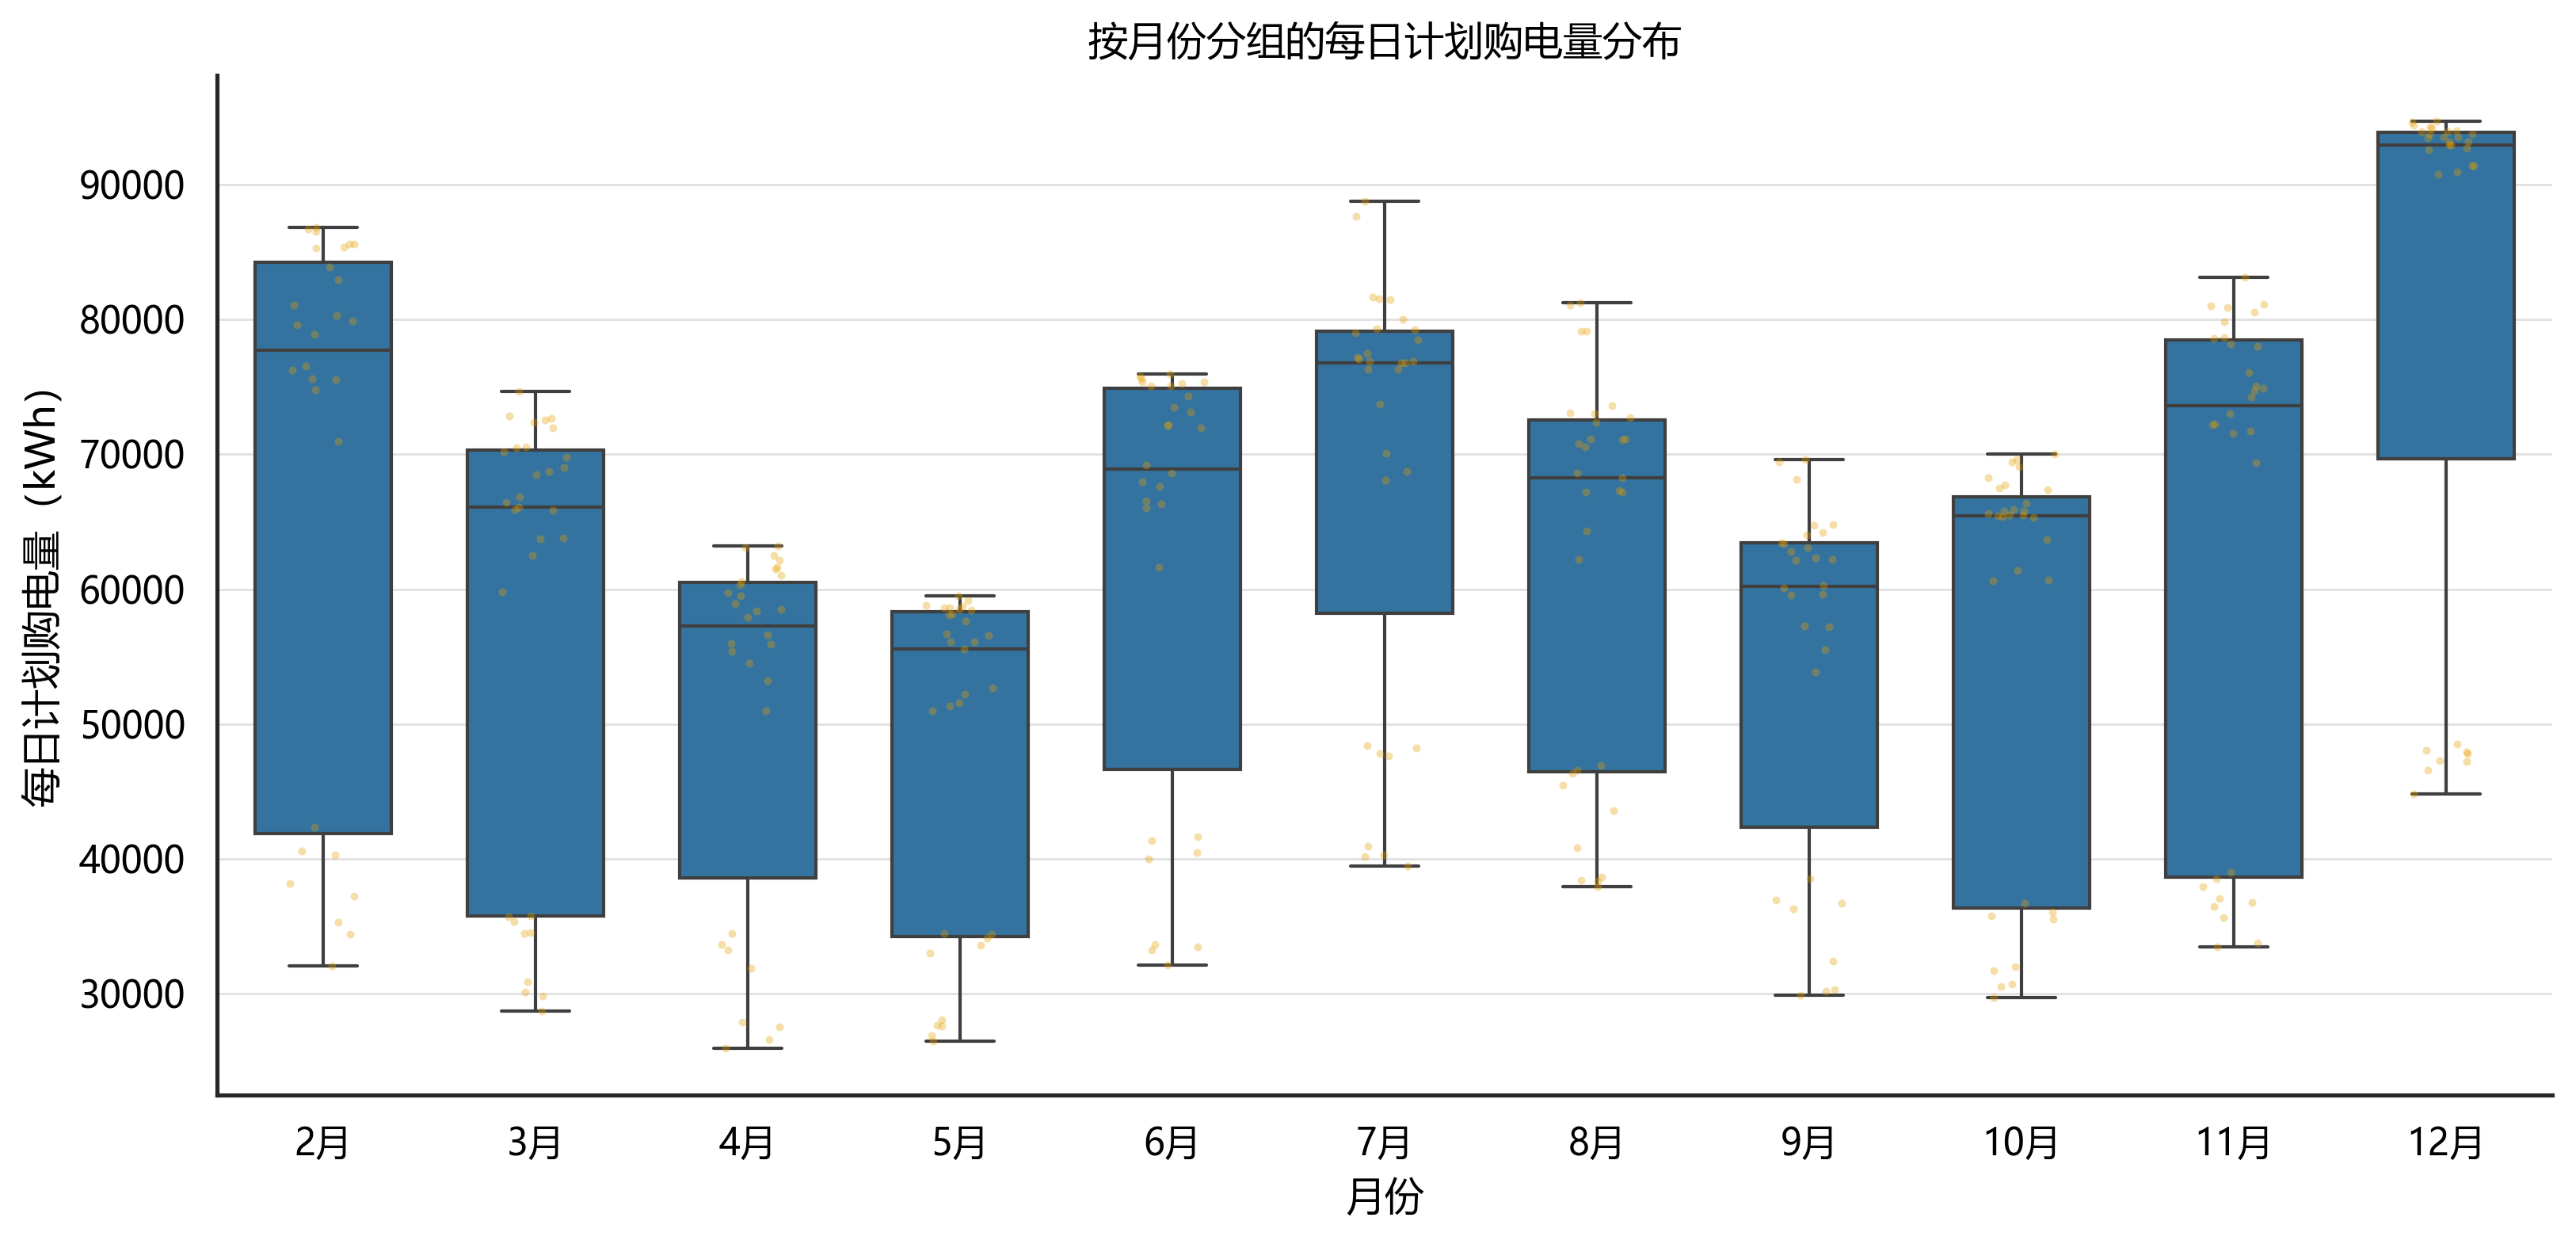
\includegraphics[width=0.49\textwidth]{figures/fig3_monthly_plan_boxplot.png}}
    \hfill
    \subfloat[全年计划购电时段热力图]{\label{fig:q2-annual-heatmap}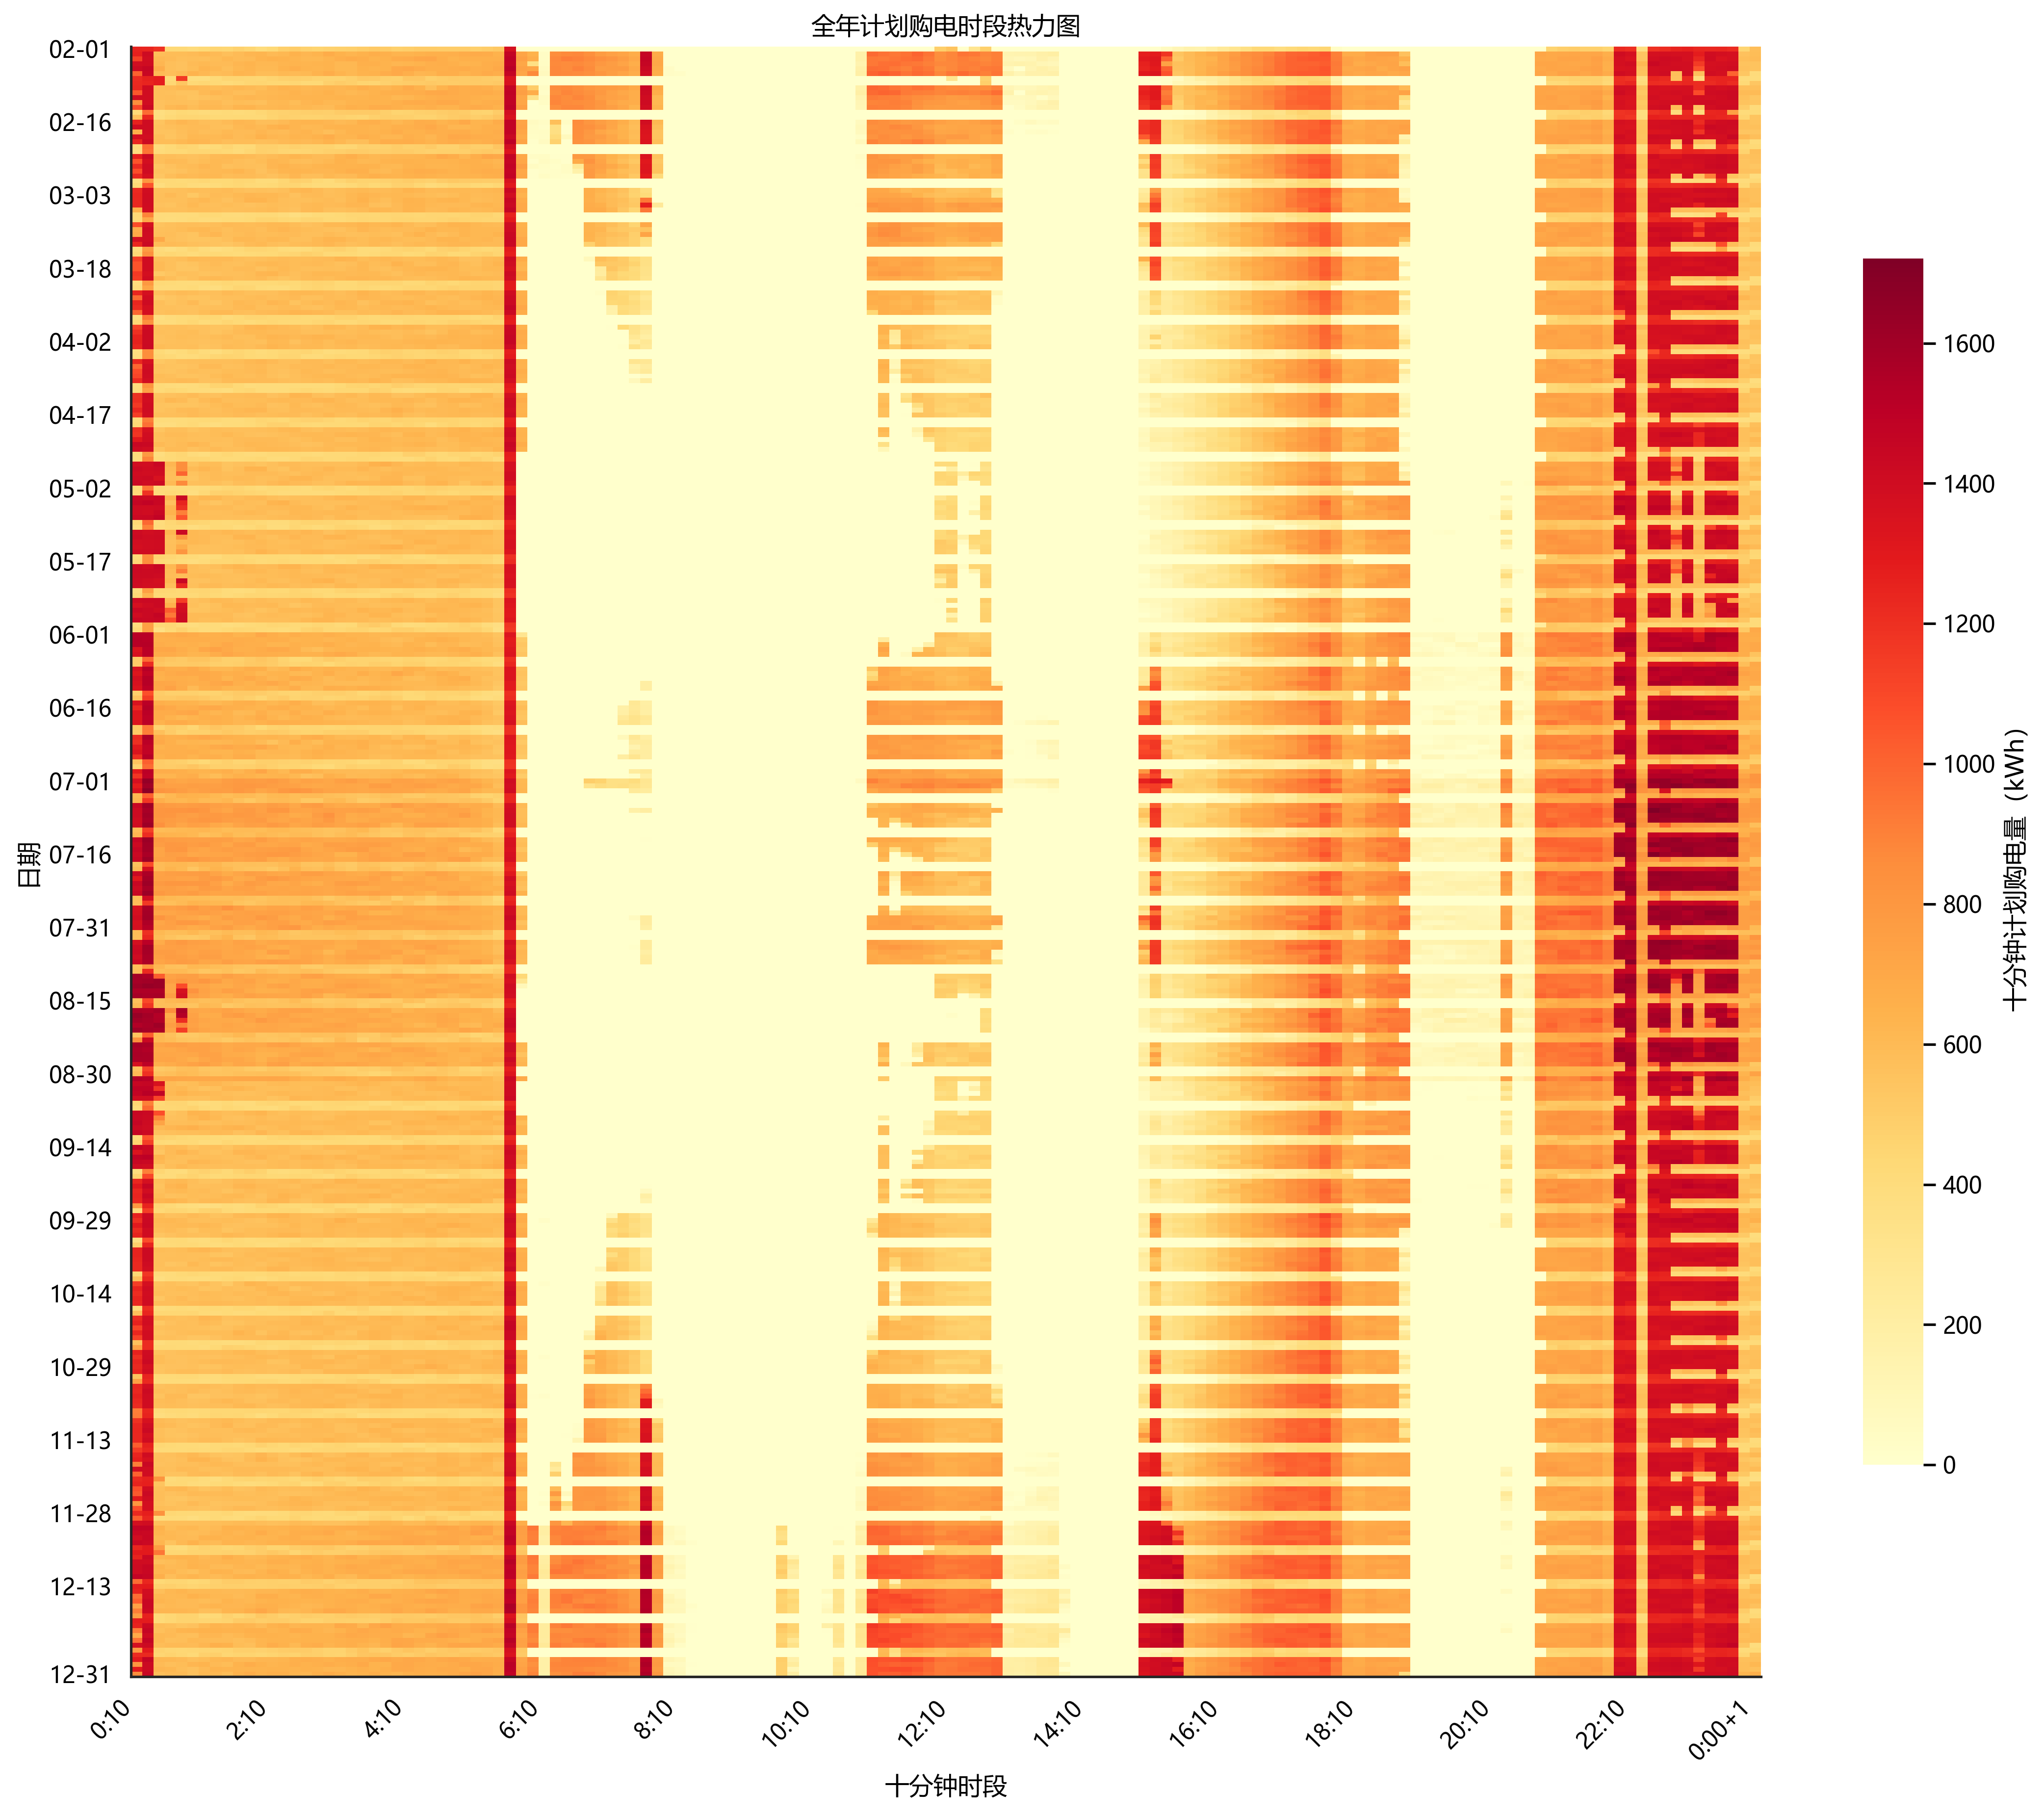
\includegraphics[width=0.49\textwidth]{figures/fig4_annual_plan_heatmap.png}}
\end{figure}

\begin{figure}[H]
    \centering
    \subfloat[指定日期计划购电曲线]{\label{fig:q2-selected-dates}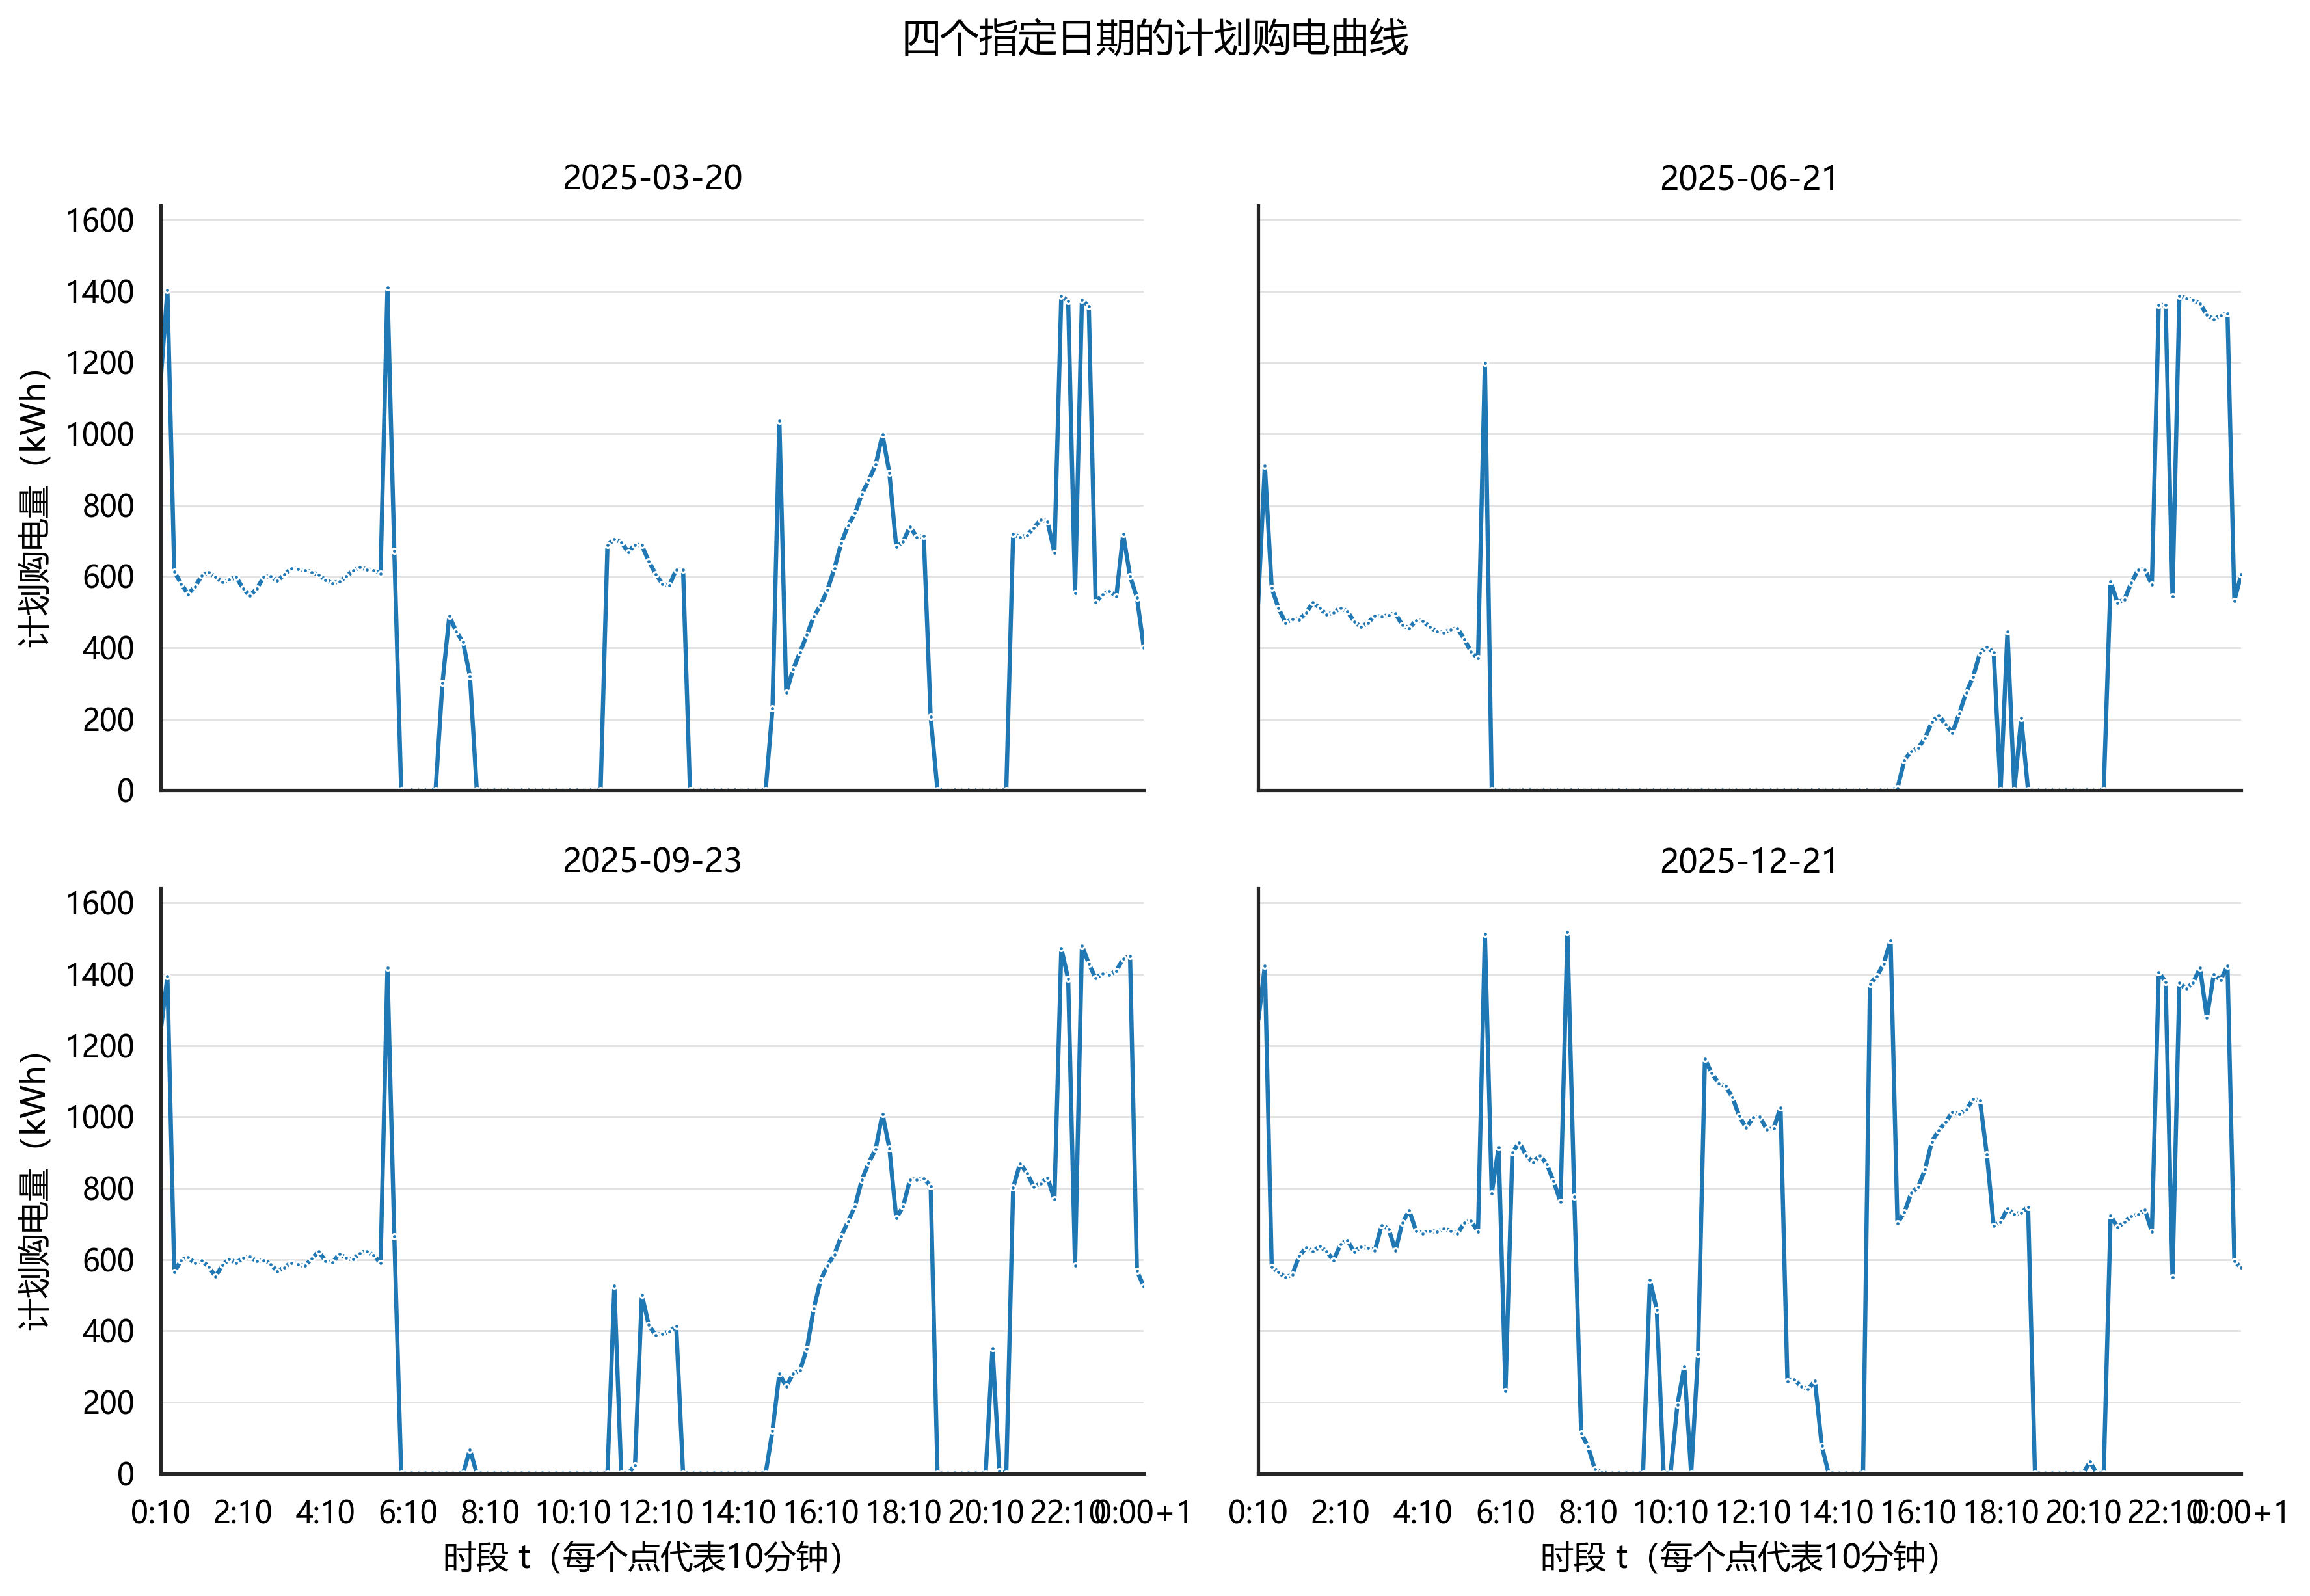
\includegraphics[width=0.49\textwidth]{figures/fig5_selected_dates_plan_curves.png}}
    \hfill
    \subfloat[计划购电量与电价关系]{\label{fig:q2-plan-vs-price}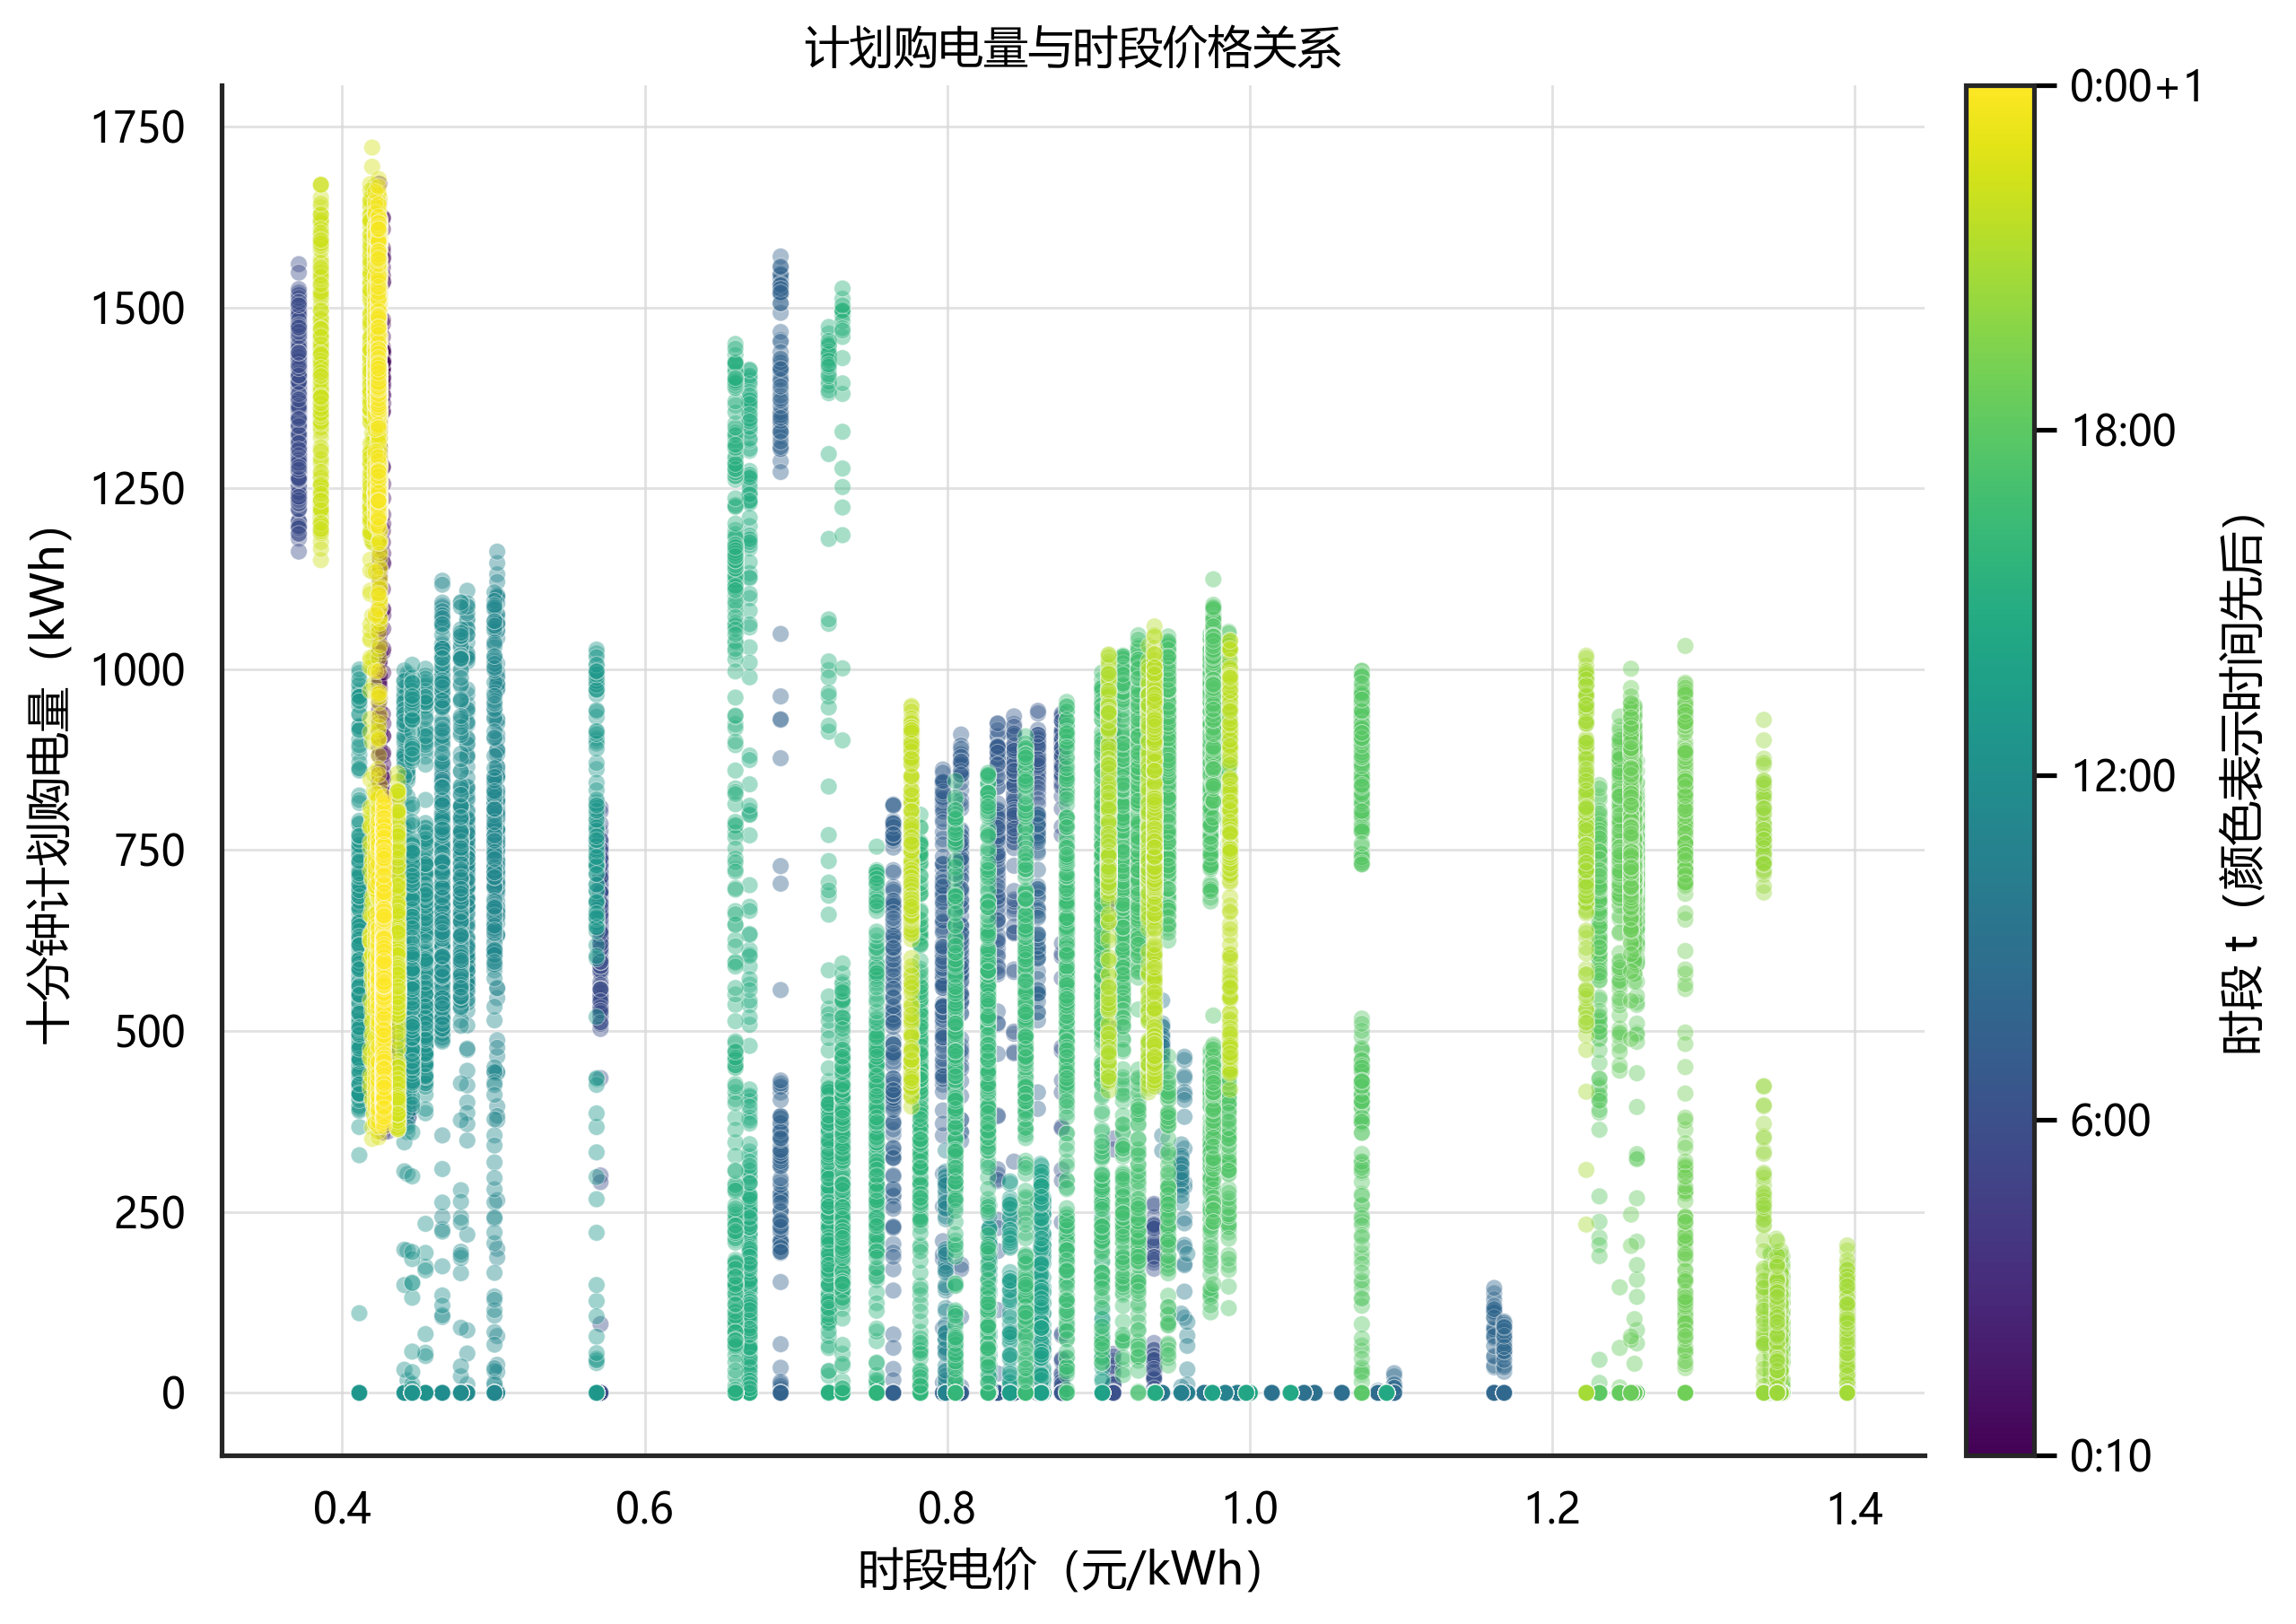
\includegraphics[width=0.49\textwidth]{figures/fig6_plan_vs_price.png}}
\end{figure}

由图 \ref{fig:q2-daily-plan-cost} 和图 \ref{fig:q2-daily-plan-calendar} 可见，计划购电在全年呈现明显季节波动：冬季和夏末购电量较高，午间低价时段购电计划相对集中。图 \ref{fig:q2-monthly-boxplot} 进一步给出各月每天计划购电的分布特征：冬季中位数和箱体均偏高，反映采暖负载大、光伏不足；夏季中位数较低，但存在个别高值异常点，对应多云或阴雨导致光伏出力骤降的日期。图 \ref{fig:q2-annual-heatmap} 从日期×时段两个维度展示计划购电的日内高峰主要出现在清晨和傍晚，与光伏无出力或出力下降时段一致。图 \ref{fig:q2-selected-dates} 展示的题目指定日期也印证了这一点：3 月 20 日、9 月 23 日等日期在早高峰和晚高峰均安排较高计划购电，6 月 21 日因白昼较长、光伏充足，计划购电整体较低。图 \ref{fig:q2-plan-vs-price} 显示计划购电量与电价总体呈正相关：清晨和傍晚电价较高（颜色偏暗）且购电量大，午间电价低（颜色偏亮）且购电量小，说明日前计划在低价时段尽量少买、在必须覆盖负载的高峰时段多买，符合价格信号引导。

\textbf{指定日期 10 分钟计划购电量与全天合计、指定日期 4 小时充放电量与始末 SOC、指定日期紧急购电区间与电量分别见附录表\ref{tab:app-q2-plan}至表\ref{tab:app-q2-settlement}}


紧急购电集中在清晨光伏尚未出力或傍晚光伏骤降时段。9 月 23 日紧急购电量最大，可能与当天云层遮挡导致光伏出力大幅低于预测有关；6 月 21 日紧急购电最少，反映夏至前后白昼长、光伏充足的特征。

\subsection{模型检验}

\subsubsection{风险权重敏感性分析}

在固定 2025-02-01 至 2025-03-02 窗口、相同预测、场景、初始 SOC 和日内执行规则下，仅改变风险权重 $\lambda$，得到表 \ref{tab:q2-lambda-sensitivity} 的结果。

\begin{table}[H]
  \centering
  \caption{风险权重 $\lambda$ 的敏感性分析结果}
  \label{tab:q2-lambda-sensitivity}
  \small
  \begin{tabularx}{\textwidth}{CCCCC}
    \toprule
    $\lambda$ & 计划购电费（元） & 紧急购电费（元） & 总费用（元） & 紧急购电量（kWh） \\
    \midrule
    0.00 & 1,216,061.69 & 185,382.40 & 1,401,444.09 & 37,432.11 \\
    0.10 & 1,221,076.21 & 174,558.31 & 1,395,634.52 & 35,243.96 \\
    0.25 & 1,228,858.66 & 155,764.36 & 1,384,623.02 & 31,358.70 \\
    0.50 & 1,229,181.56 & 155,764.36 & 1,384,945.91 & 31,358.70 \\
    \bottomrule
  \end{tabularx}
\end{table}

由表 \ref{tab:q2-lambda-sensitivity} 可见，随着 $\lambda$ 增大，计划购电费略上升，紧急购电费和总费用先降后稳。$\lambda=0.25$ 时总费用最低；继续增大到 0.50 未进一步降低紧急购电，反而略微增加了计划购电费。因此模型采用 $\lambda=0.25$ 合理。

\section{问题三：四阶段光伏预测更新下的计划与调整购电优化}

\subsection{问题分析}

\subsubsection{决策层级与信息结构}

问题三在问题二的风险控制上进一步引入附件 3 提供的每六个小时日内光伏预测，其决策由\textbf{“阶段日前计划、日内滚动执行"扩展为"日前计划、多阶段合同调整、日内滚动执行”}的三层结构：

\begin{itemize}
    \item \textbf{00:00 日前阶段}：仅基于附件 3 当天发布的 24 小时整点预报和日前历史信息，确定当天计划购电量 $P_t$。同问题二,一旦提交不能以任何理由撤回或修改已发生的计划量。
    \item \textbf{06:00、12:00、18:00 调整阶段}：在每个更新时刻，同时更新新的 24 小时预报，针对尚未发生的时段重新优化最终生效购电量 $A_t$。
    \item \textbf{10 分钟执行阶段}：实际光伏每 10 分钟揭示一次，执行当前时段储能充放电、弃光、未利用计划购电和紧急购电，后重新求解剩余时段。
\end{itemize}

特别地，附件 3 在 00:00 只给出当天 24 小时预报，因此第一阶段计划模型是问题二风险日前 LP 的\textbf{单日情况}，不能虚构未来两天的预报数据。

问题三在问题二的权衡之上，当实际调整量 $A_t$ 小于计划量 $P_t$，少买部分按半价 $0.5p_t$ 结算偏差；当实际调整量 $A_t$ 大于计划量 $P_t$ 时，多买部分按 1.5 倍电价 $1.5p_t$ 结算偏差。这一机制使模型过度激进的计划会在光伏好于预期时产生大量半价损失；过度保守的计划则会在光伏差于预期时被迫高价购电，最优计划量应处于"覆盖基准负载风险"与"保留调整灵活性"之间。

06:00、12:00、18:00 的预报更新能够逐步修正光伏预测误差，使调整购电量 $A_t$ 更接近实际光伏，但更新次数过度增加会提高模型复杂度的同时提升效益甚微。因此需要通过消融实验确定保留哪些更新时刻。

\subsection{模型建立}

\subsubsection{四阶段预测与调整策略结构}

附件 3 在 $r\in\{0,6,12,18\}$ 发布未来 24 小时整点功率预报 $\hat R_h^{(r)}$。将其展开为 10 分钟电量，并以后发布覆盖前发布的原则构造预测曲线：
\begin{equation}
\hat R_t=\hat R_t^{(r)}, \quad t\ge 6r.
\end{equation}

对 $r=6,12,18$，用目标日前同发布时间历史预报误差的 0.30 分位数\textsuperscript{[6]}修正未来预报：
\begin{equation}
\tilde R_h^{(r)} = \max\bigl(0,\;\hat R_h^{(r)}+Q_{0.30}(\varepsilon_{d',h}^{(r)})\bigr), \quad d'<d.
\end{equation}

\subsubsection{三层随机优化}

\textbf{00:00 风险日前计划。} 以附件 3 当天 24 小时预报为输入，调用问题二风险日前 LP 的单日特例，得到当日计划购电量 $P_t$。保留历史误差场景压缩（$\le12$ 组）、低光伏压力场景（概率 0.10）、CVaR$_{0.90}$（$\lambda=0.25$）、场景树非预见性约束。
\textbf{06:00/12:00/18:00 调整。} 仅对未发生时段 $t\in\mathcal T_r=\{6r,\dots,144\}$ 重新优化最终购电量 $A_t$，已发生时段不变。引入 $u_t,v_t\ge0$ 使
\begin{equation}
A_t+u_t-v_t=P_t,\quad t\in\mathcal T_r,
\end{equation}
主结算费用为
\begin{equation}
\begin{aligned}
C_t^{\rm normal}
&=p_tA_t+0.5p_tu_t+0.5p_tv_t\\
&=p_t\min(P_t,A_t)+0.5p_t(P_t-A_t)^+
 +1.5p_t(A_t-P_t)^+.
\end{aligned}
\end{equation}
\vspace{5pt}
调整阶段以风险感知目标最小化正常结算、期望紧急购电（5 倍电价）及 CVaR 尾部费用（同问题二），并满足非预见性约束。

\textbf{10 分钟因果滚动执行。} 每 10 分钟获得真实光伏 $R_t$ 后，仅优化并执行当前时段控制。能量平衡为
\begin{equation}
A_t+R_t+d_t+e_t=L_t+c_t+w_t^{PV}+w_t^{grid},
\end{equation}
并满足 $0\le w_t^{PV}\le R_t$，$0\le w_t^{grid}\le A_t$，禁止同时充放电，紧急购电仅补负载缺口。

正式结果采用主结算口径 $C_t^{\rm normal}$；备用口径（计划量全额结算后再叠加偏差）仅作敏感性参考。


\subsection{模型求解与结果分析}

\subsubsection{全年结果}
运行上述四阶段预测更新框架，得到 2025 年 2 月 1 日至 12 月 31 日共 334 天的购电、调整策略结果，如表 \ref{tab:q3-annual-summary} 所示。
\begin{table}[H]
    \centering
    \caption{问题三全年运行结果}
    \label{tab:q3-annual-summary}
    \small
    \begin{tabularx}{\textwidth}{CC}
        \toprule
        指标 & 结果 \\
        \midrule
        计划购电量 & 21,427,841.32 kWh \\
        计划购电费 & 13,111,843.82 元 \\
        调整后购电量 & 21,388,073.72 kWh \\
        计划加调整结算费 & 13,641,253.25 元 \\
        调整偏差费用 & 949,015.77 元 \\
        紧急购电量 & 61,376.99 kWh \\
        紧急购电费（估计） & 281,152.00 元 \\
        总购电费用估计 & 13,922,405.25 元 \\
        紧急购电天数 & 296 天 \\
        最大供需平衡误差 & 约 $10^{-8}$ kWh \\
        同时充放电时段 & 0 \\
        \bottomrule
    \end{tabularx}
\end{table}


与\textbf{问题二的最终结果}（总费用 13,731,036.47 元、紧急购电 159,973.16 kWh）相比，问题三总费用为 13,922,405.25 元，上升约 19.14 万元（约 1.39\%）；但紧急购电量下降约 9.86 万 kWh（约 61.63\%）。总费用的小幅上升来自日内调整偏差的结算成本，日内更新以该成本换取紧急购电风险的大幅下降，说明日内更新的核心价值在于降低供电风险。
\subsubsection{指定日期总电费与紧急购电分析}

\textbf{3 月 20 日、6 月 21 日、9 月 23 日、12 月 21 日各天总电费、紧急购电量及购电情况见附录表\ref{tab:app-q3-plan}至表\ref{tab:app-q3-settlement}。}
四个指定日期的详细计划购电、调整购电、紧急购电及费用结果见附录表。总体上，光伏充足日期的日内调整能够降低紧急购电，但在光伏波动较大或负荷较高的日期仍可能保留少量紧急购电；调整偏差费用也可能抵消部分费用节省。因此，日内更新的主要作用是降低供电风险，而不是保证每个指定日期的总费用都下降。

\subsubsection{结果可视化}

图 \ref{fig:q3-daily-plan-adjusted}--\ref{fig:q3-q2-q3-cost} 给出问题三关键结果可视化。

\begin{figure}[H]
    \centering
    \subfloat[全年逐日计划购电量与调整购电量]{\label{fig:q3-daily-plan}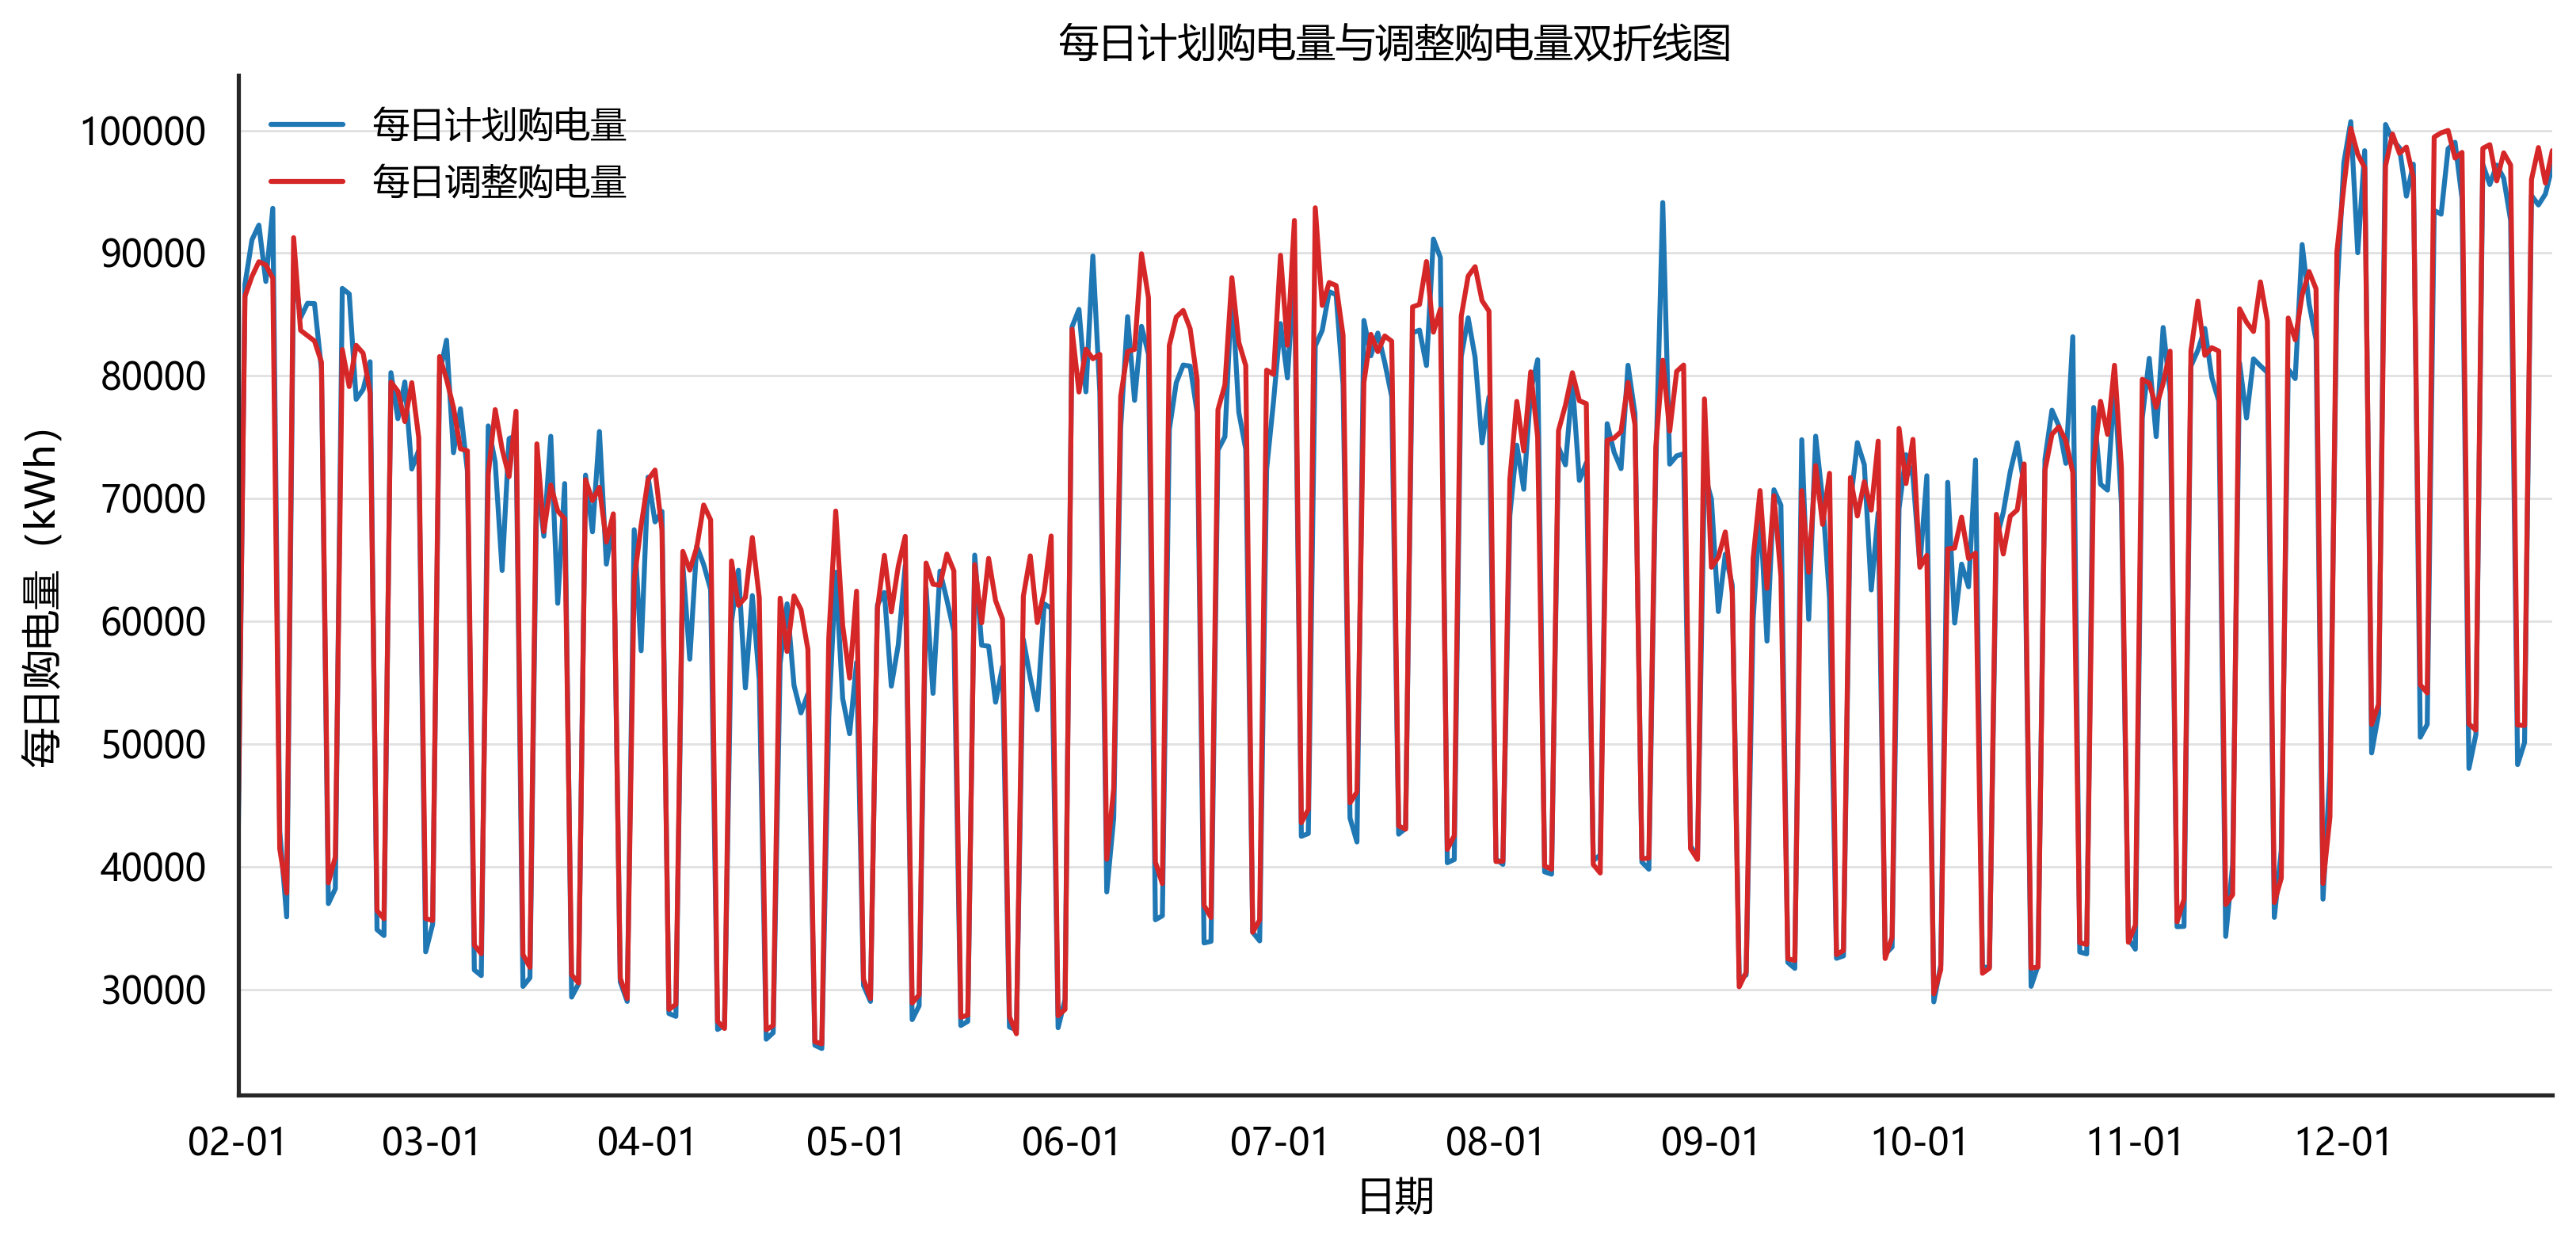
\includegraphics[width=0.49\textwidth]{figures/图10.png}}
    \hfill
    \subfloat[每天调整结算费用]{\label{fig:q3-daily-adjusted-cost}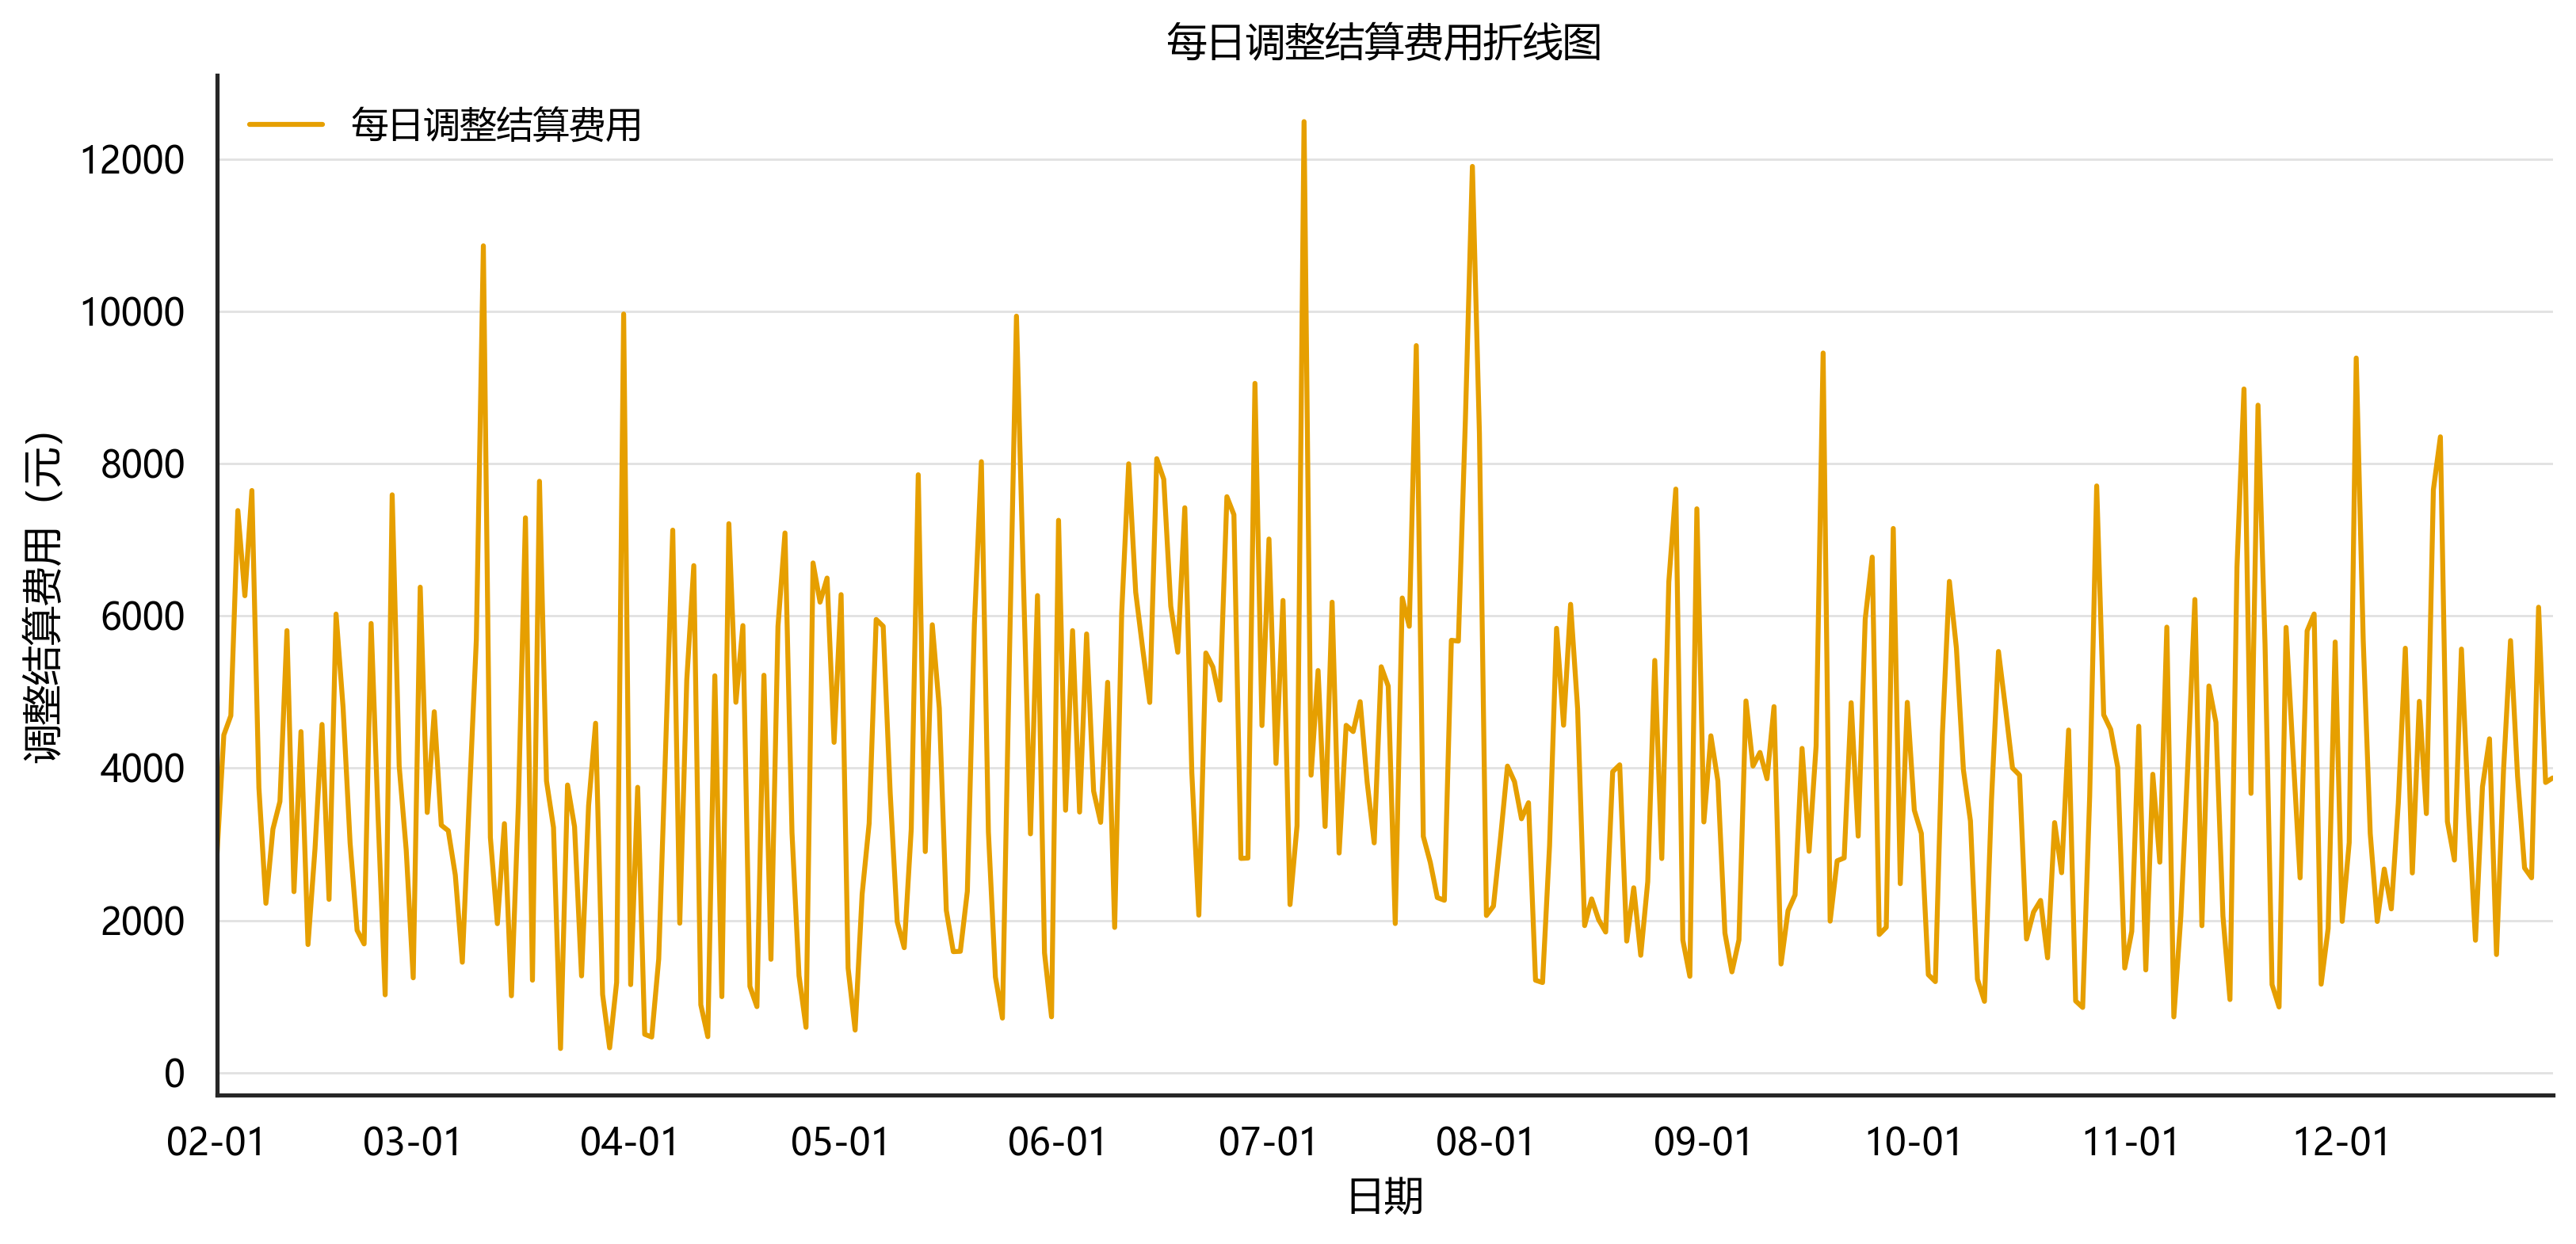
\includegraphics[width=0.49\textwidth]{figures/图11.png}}
    \caption{全年逐日计划购电量、调整购电量及每日调整结算费用}
    \label{fig:q3-daily-plan-adjusted}
\end{figure}

调整购电量在多数日期与计划量相近，在光伏波动较大的日期内会有明显偏离；调整结算费用在光伏剧烈波动日出现明显尖峰。从全年数据来看，每天净调整比例中位数约 0.6\%、均值约 0.2\%，绝对调整比例中位数约 5.0\%、均值约 5.8\%，调整机制主要用于修正白天的光伏预测误差而非大幅改变日前计划。

\begin{figure}[H]
    \centering
    \subfloat[指定日期计划购电量、调整购电量与购电偏差]{\label{fig:q3-selected-dates-triptych}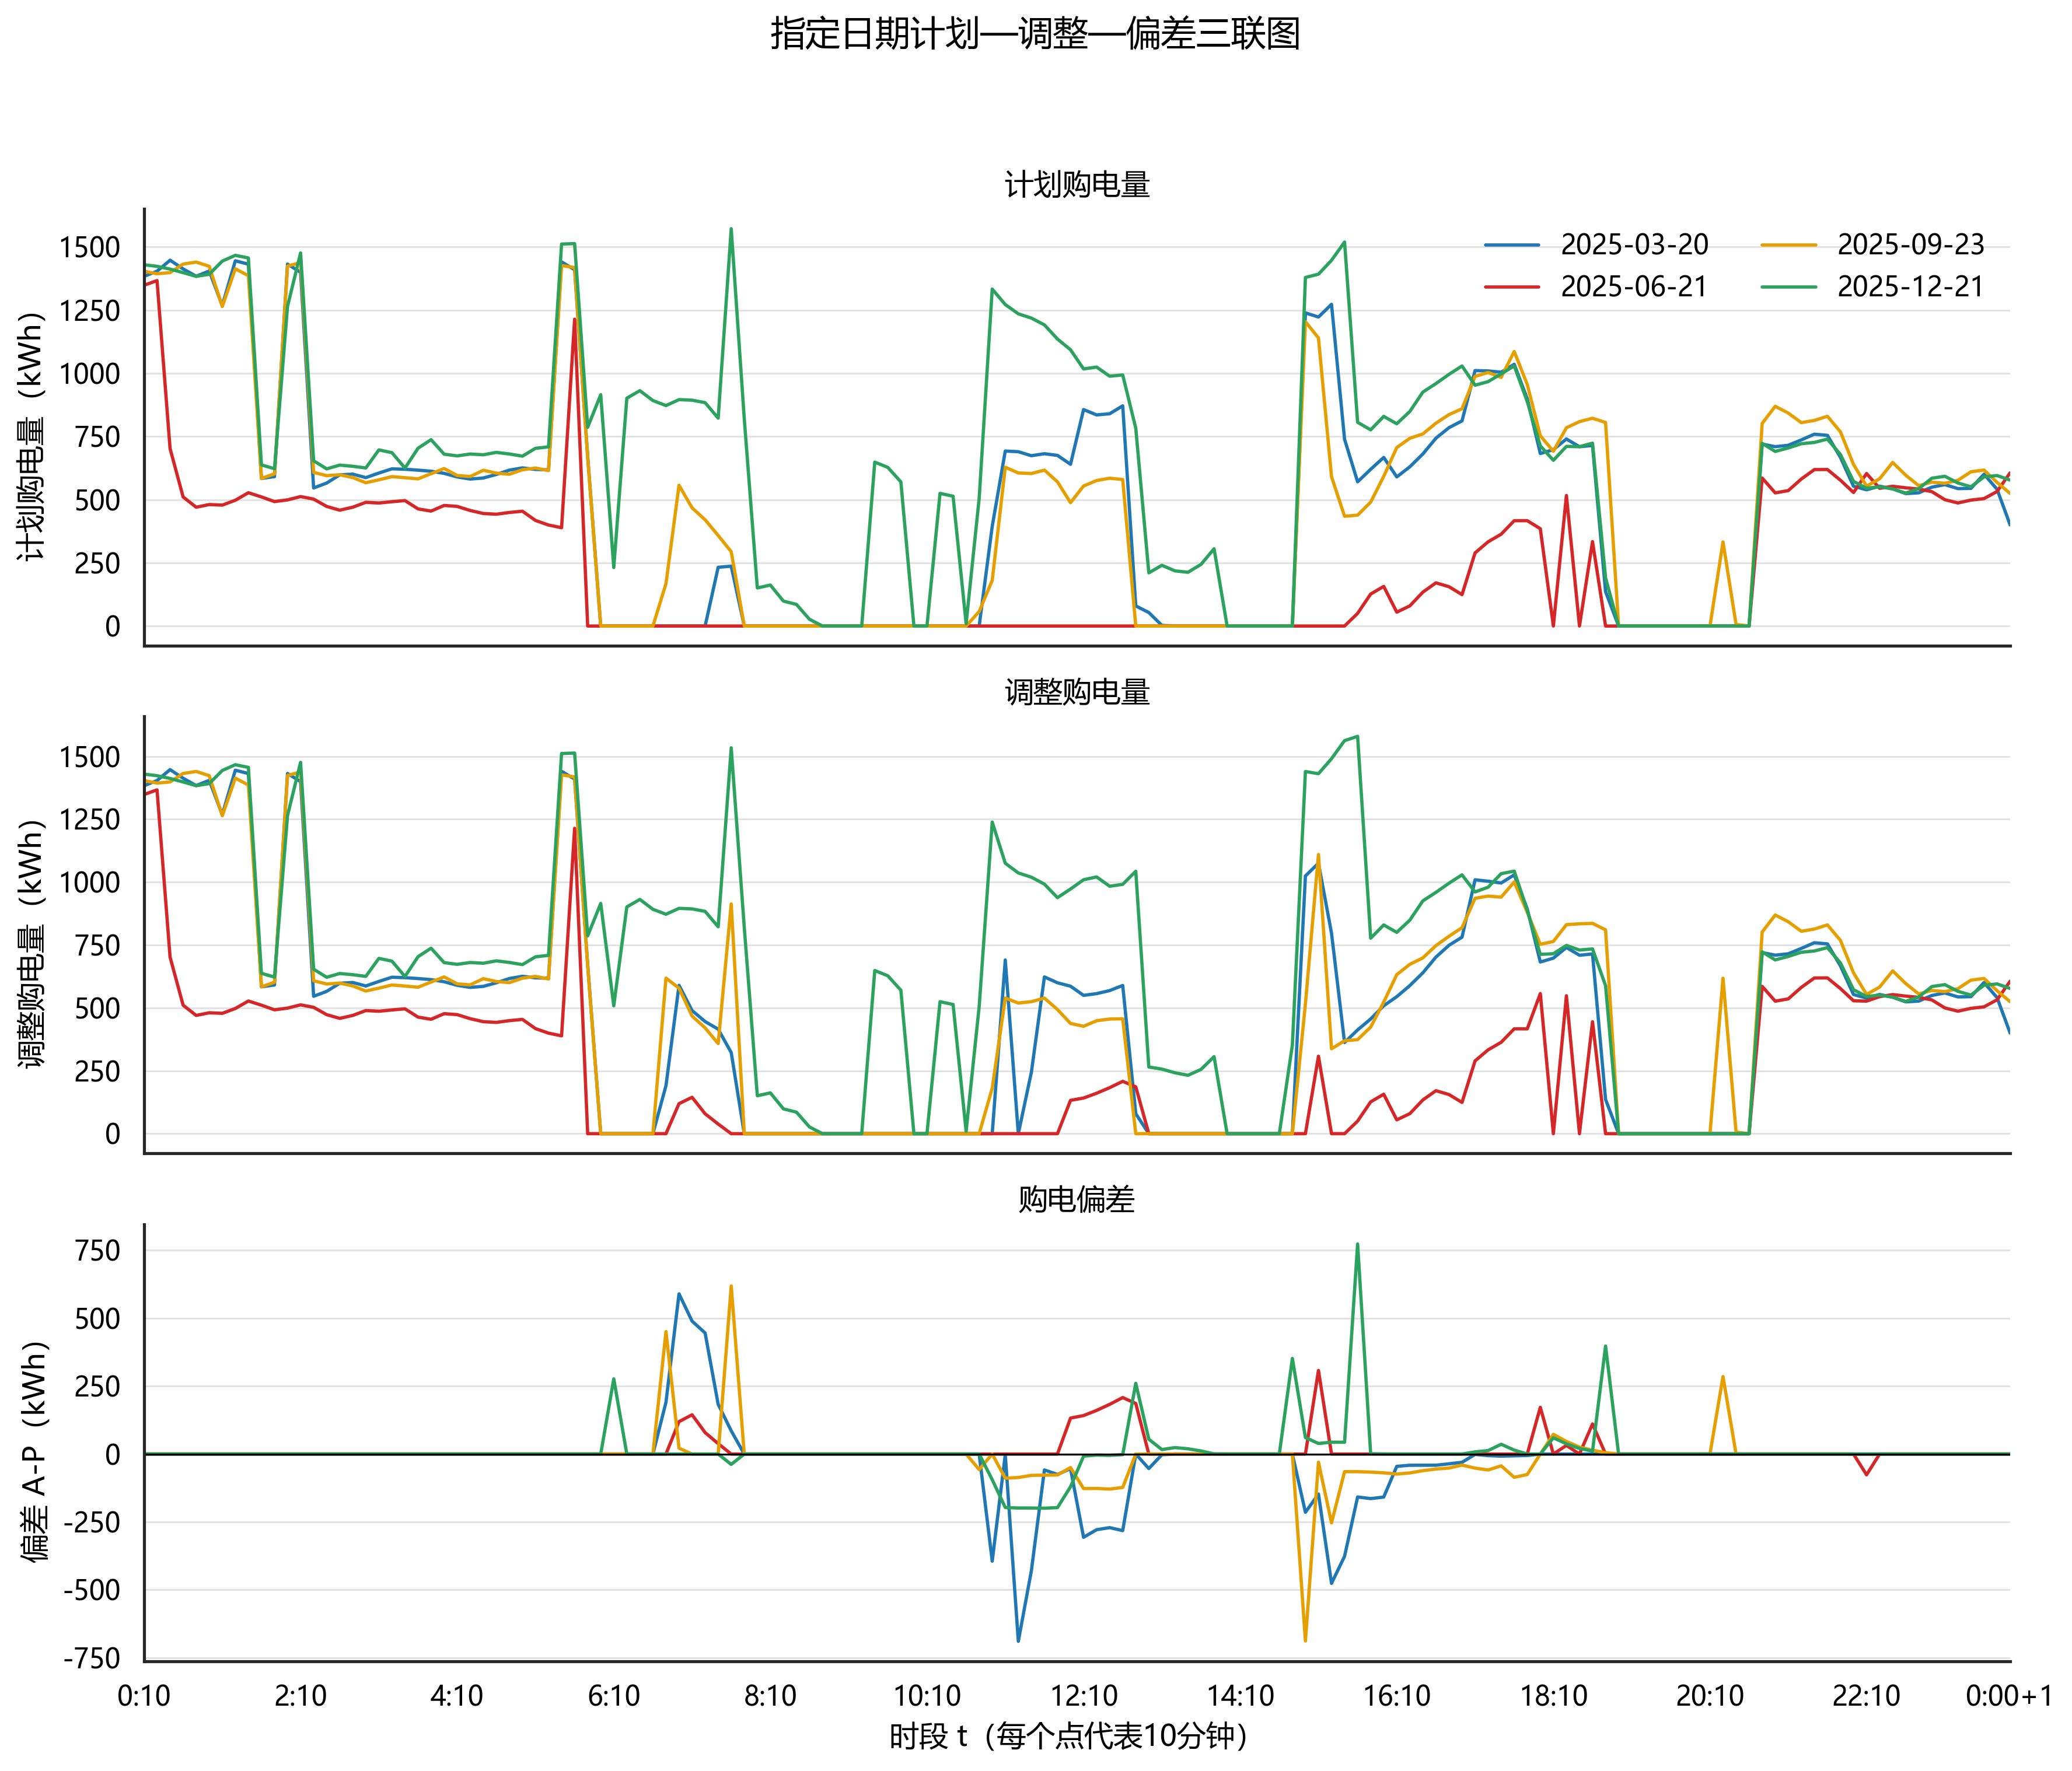
\includegraphics[width=0.49\textwidth]{figures/图12.png}}
    \hfill
    \subfloat[全年日期—时段购电调整量热力图]{\label{fig:q3-adjustment-heatmap}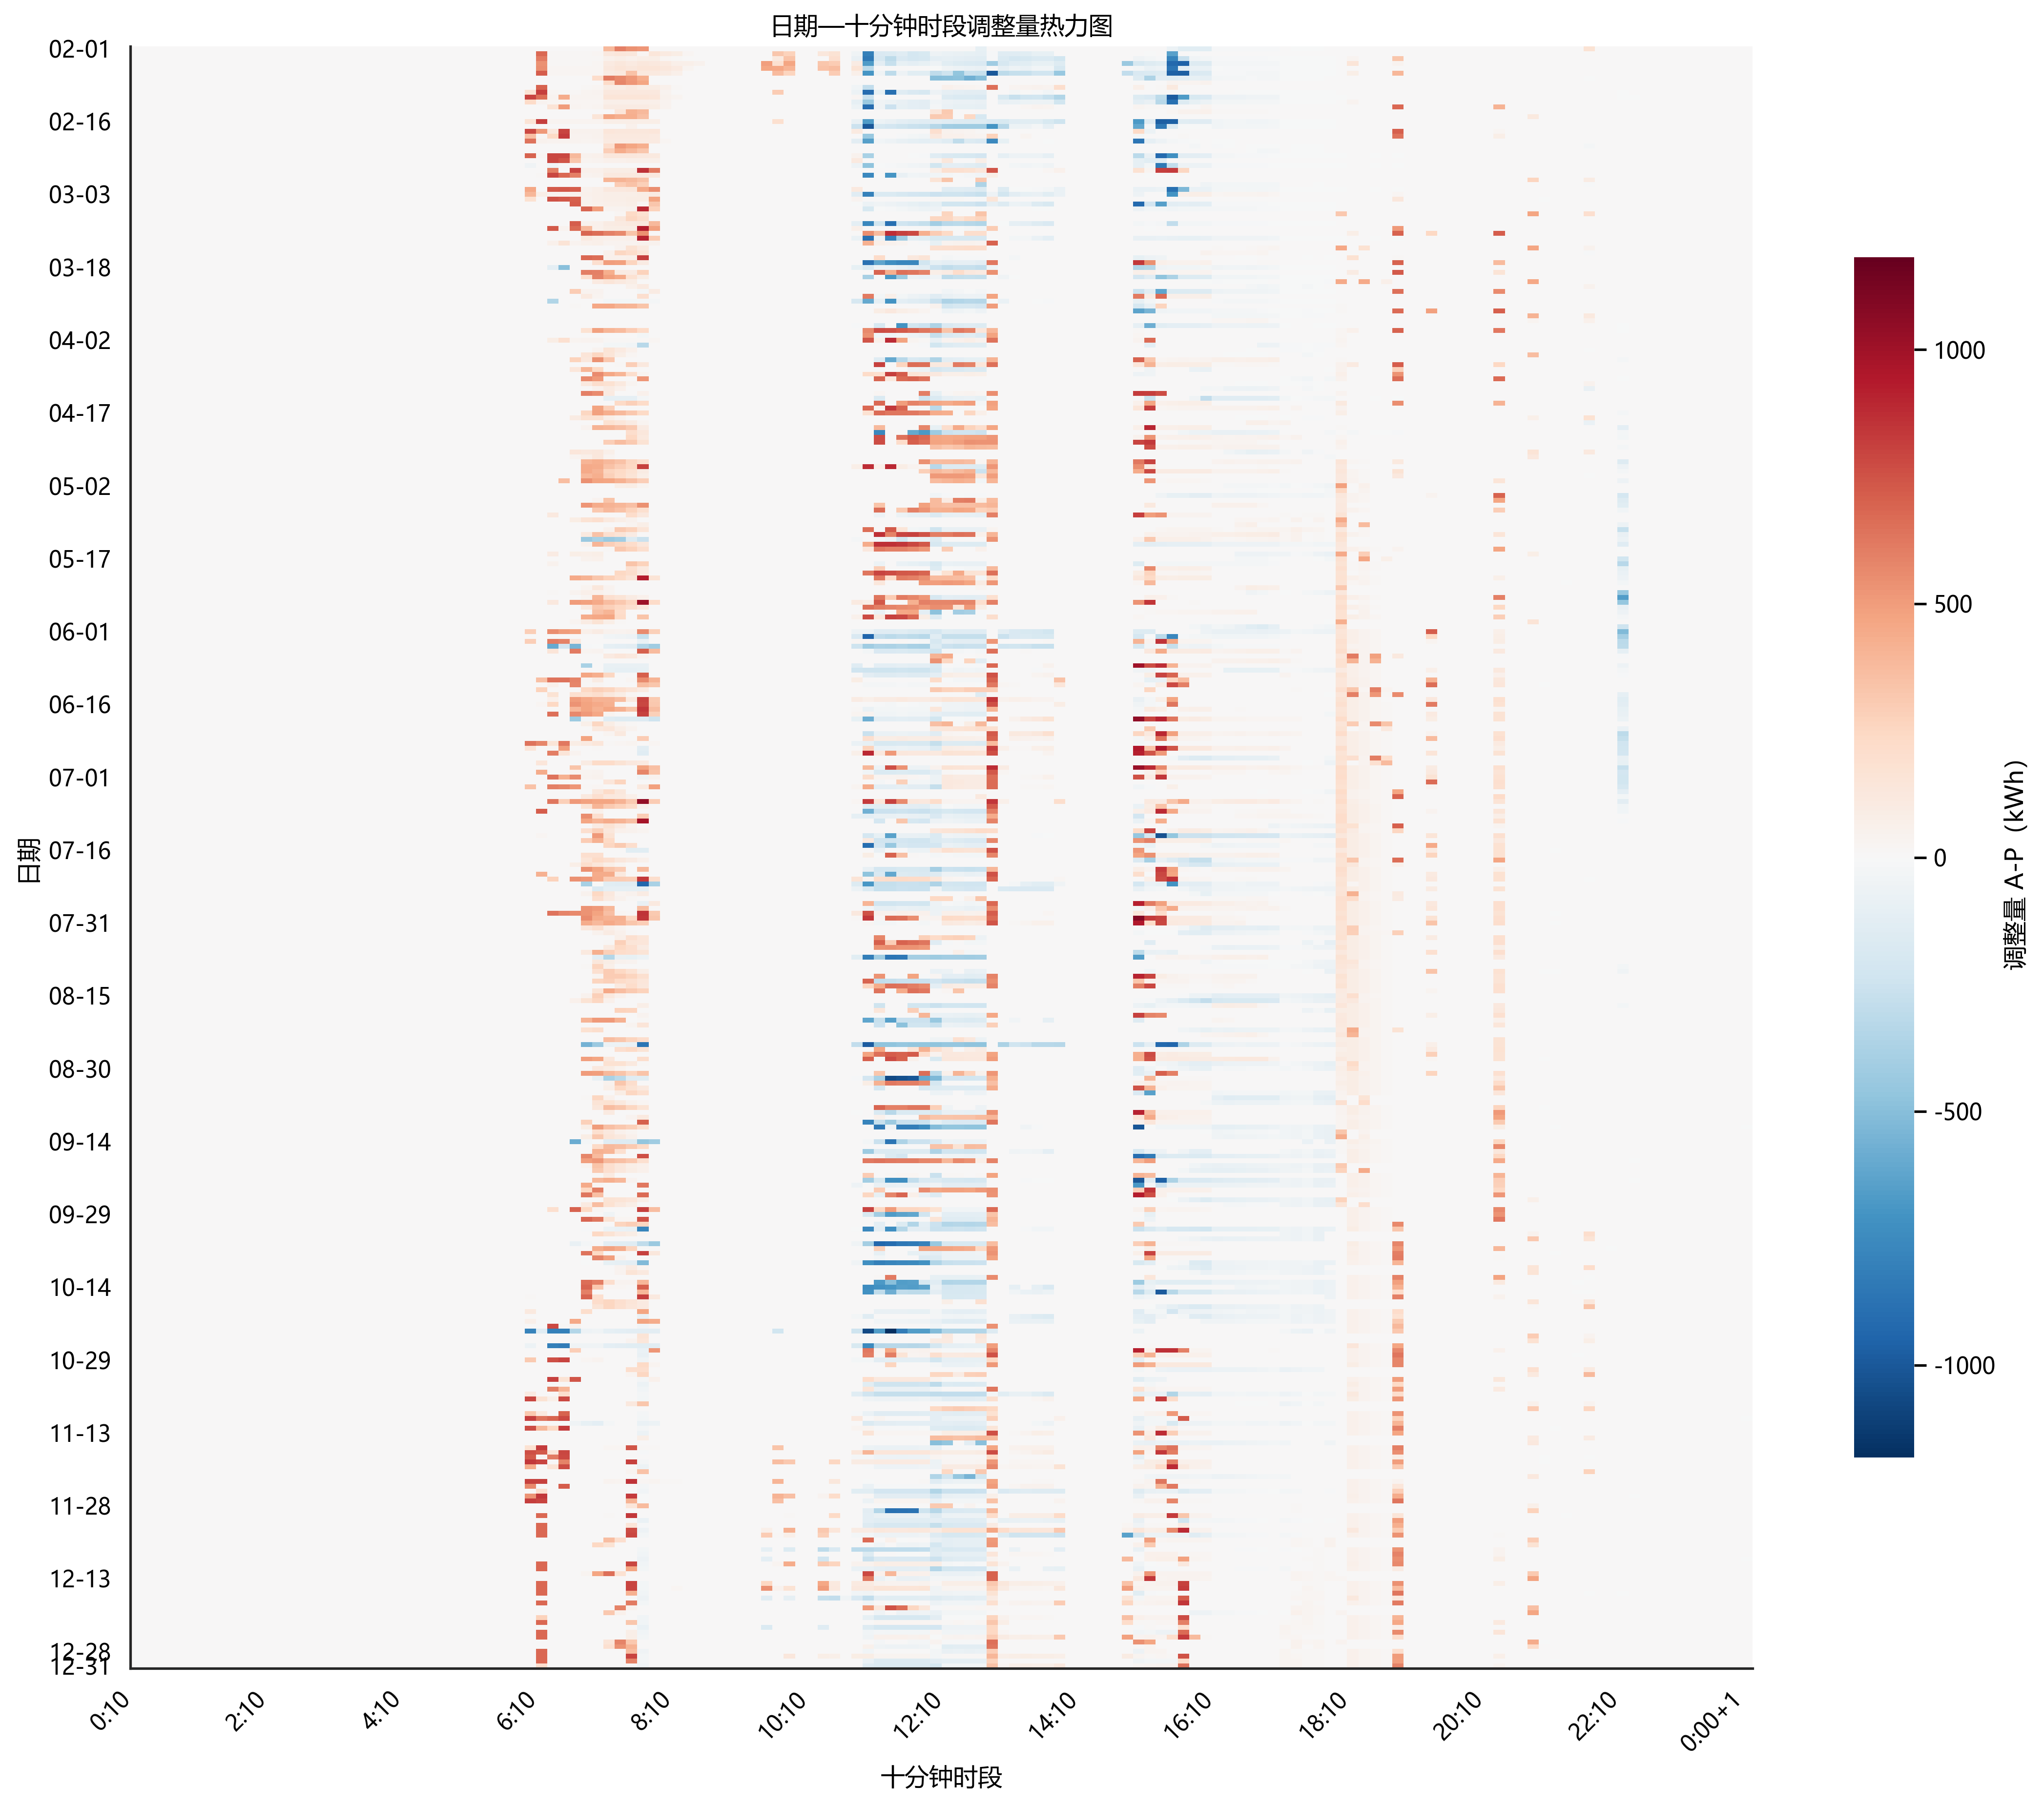
\includegraphics[width=0.49\textwidth]{figures/图13.png}}
    \caption{指定日期购电偏差与全年调整量分布}
\end{figure}

图 \ref{fig:q3-selected-dates-triptych} 显示 6 月 21 日计划与调整在数值上几乎重合，而 12 月 21 日早间和傍晚调整量显著高于计划，反映日内预报对高负载时段有修正作用。图 \ref{fig:q3-adjustment-heatmap} 显示调整量除了在早晨傍晚会有上调，在\textbf{正午}这一光伏功率不确定的时段也会做出调整，\textbf{夏末、秋初、冬季的调整幅度明显大于其他时期}。

\begin{figure}[H]
    \centering
    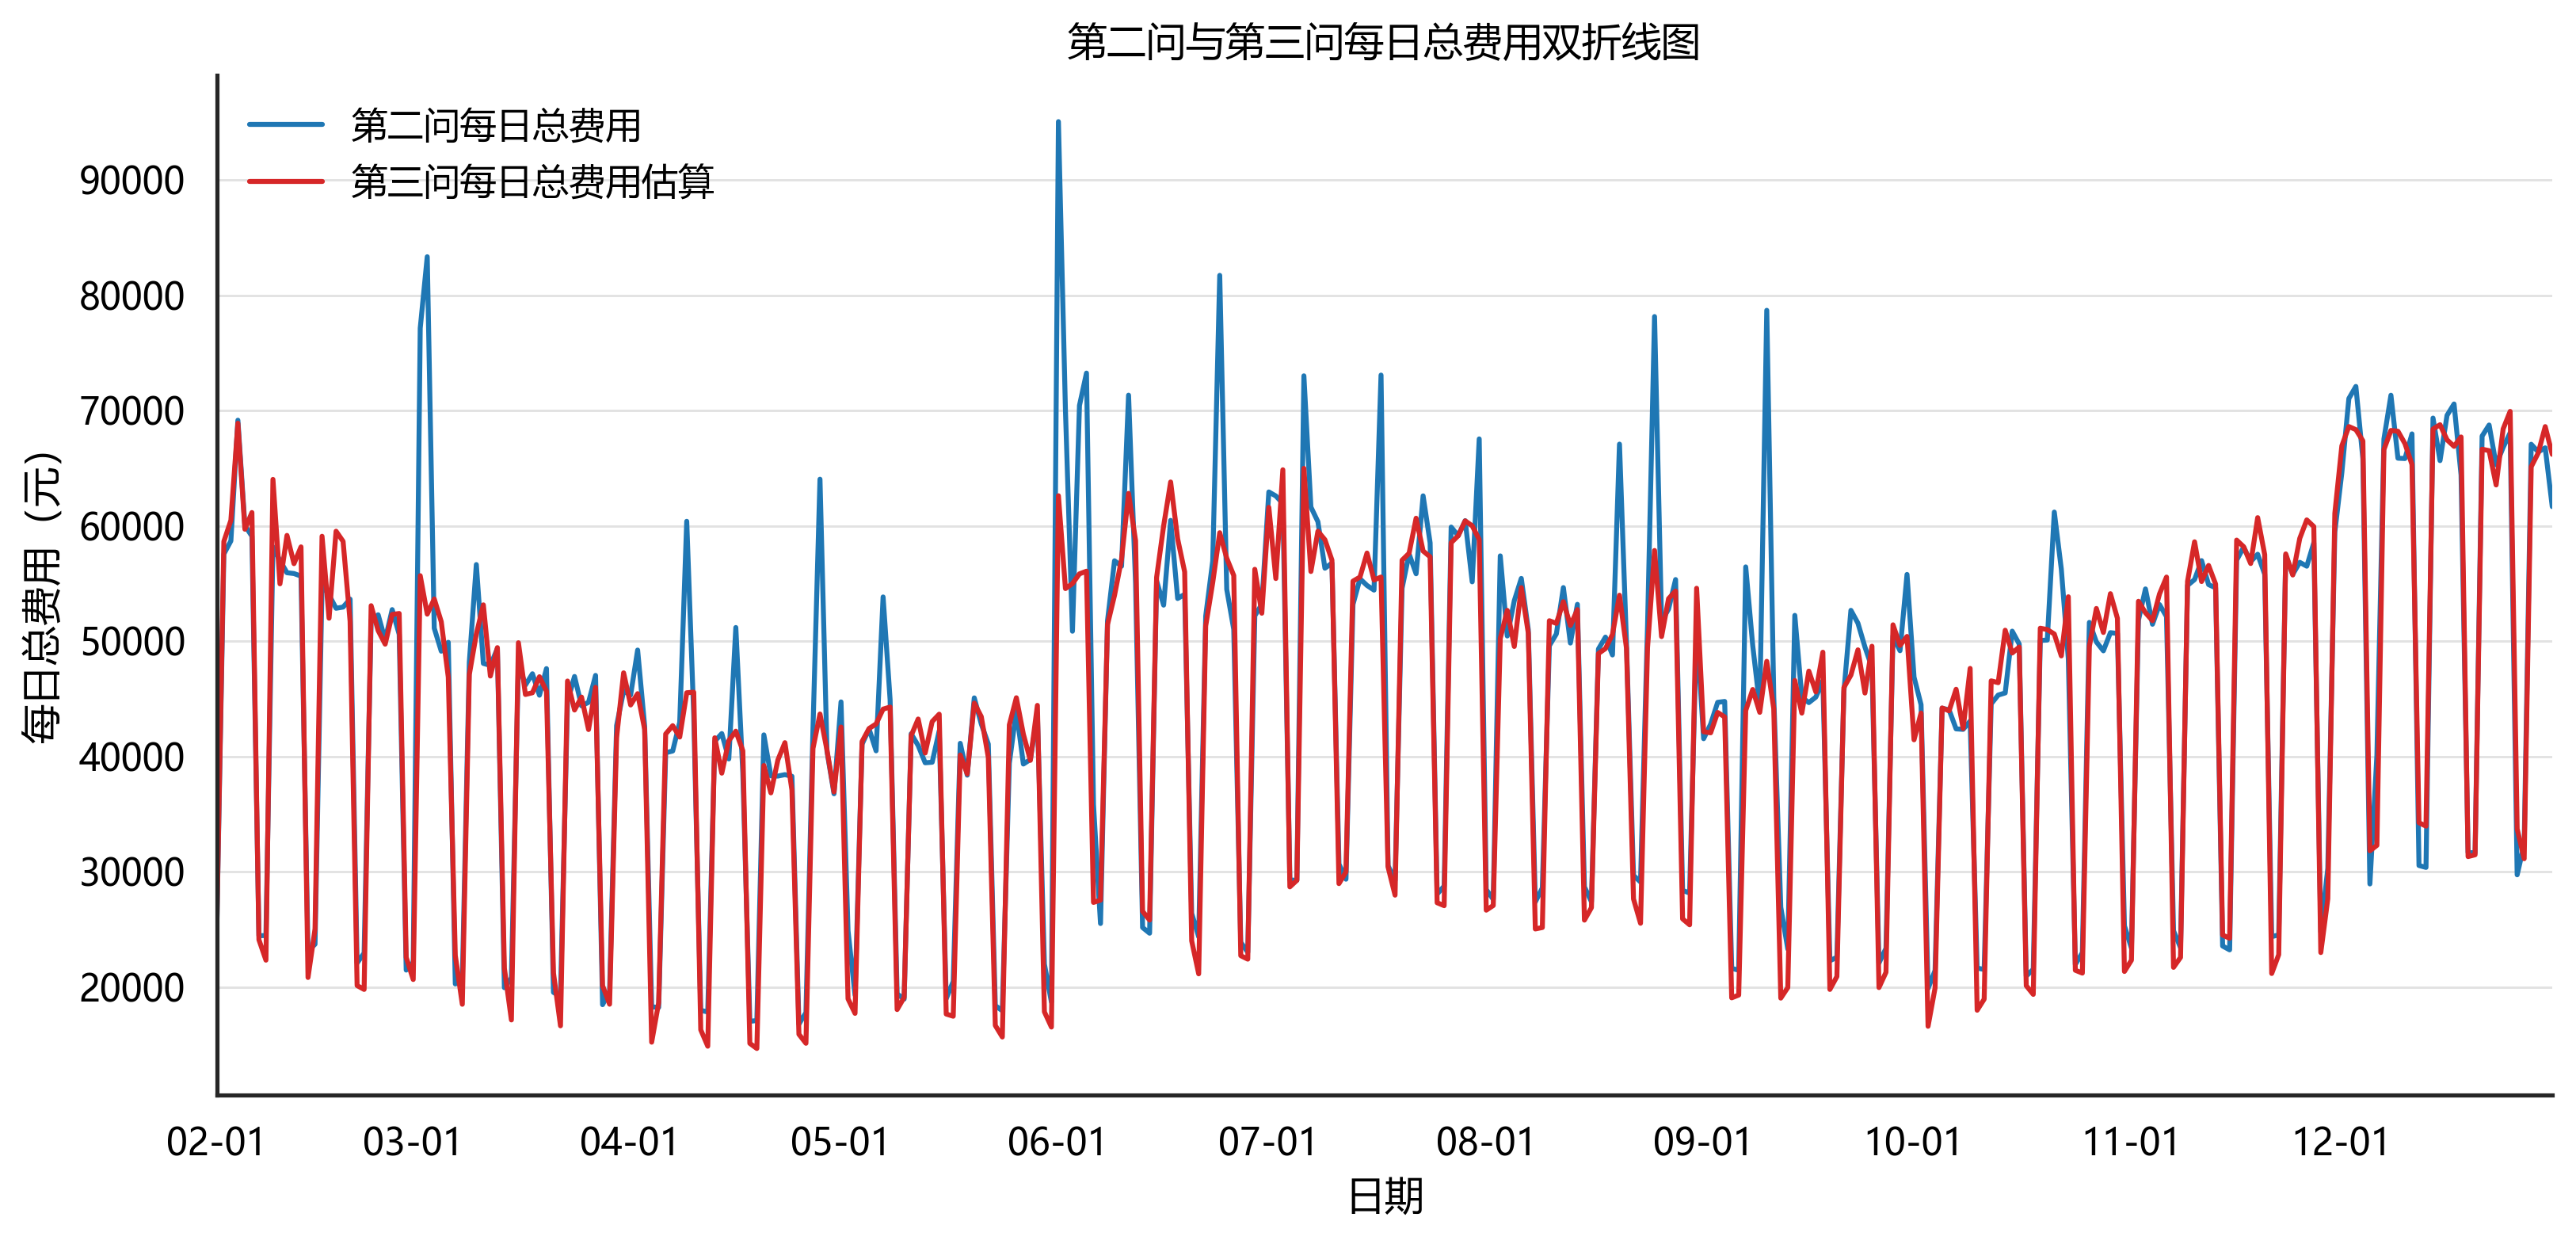
\includegraphics[width=0.6\textwidth]{./figures/图14.png}
    \caption{问题二与问题三逐日总费用对比}
    \label{fig:q3-q2-q3-cost}
\end{figure}

图 \ref{fig:q3-q2-q3-cost} 显示第三问相比于第二问以 19.14 万元的调整结算成本为代价，大幅削减了因紧急购电带来的尖峰费用。

其他必要结果已保存至 result3.xlsx中。、
\subsection{日内预报更新时刻的使用价值分析}

本节从\textbf{实际预测准确性}、\textbf{白天快速变化窗口}、\textbf{相邻发布时刻预测改善}、\textbf{发布时间之后经济暴露}以及\textbf{现有发布时刻消融}五个角度，评价 00:00、06:00、12:00、18:00 四个发布时刻的价值。
\textbf{（1）实际预测准确性}。06:00 因提前覆盖上午光伏爬坡且尚未受午后影响，MAE 最低；12:00、18:00 MAE 较高，说明午后至傍晚不确定性显著；各时刻均呈正偏差，存在低估风险。

\textbf{（2）白天快速变化窗口}。06:00 在上午 07:00--10:00 窗口将低估率从 8.86\% 降至 2.10\%，紧急风险代理从 139.36 降至 16.94，价值最大；14:00--18:00 各发布时刻低估率均接近 1，是风险最高窗口。

\textbf{（3）相邻发布时刻的预测改善}。表 \ref{tab:q3-forecast-gain} 给出相同日期、相同目标小时的配对比较。00:00$\rightarrow$06:00 与 12:00$\rightarrow$18:00 的 MAE 改善较大，但 Bootstrap 区间较宽且后发布更准确比例未过半，说明改善存在但受日期和目标小时异质性影响。

\begin{table}[H]
  \centering
  \caption{相邻发布时刻预测改善配对}
  \label{tab:q3-forecast-gain}
  \small
  \begin{tabularx}{\textwidth}{CCCCC}
    \toprule
    更新对 & 共同目标小时数 & MAE 改善（kW） & 后发布更准确比例 & Bootstrap 区间（kW） \\
    \midrule
    00:00$\rightarrow$06:00 & 18 & 54.19 & 34.06\% & $[-45.997,\;267.394]$ \\
    06:00$\rightarrow$12:00 & 18 & 21.77 & 18.66\% & $[-18.978,\;232.318]$ \\
    12:00$\rightarrow$18:00 & 18 & 71.79 & 20.46\% & $[-18.263,\;689.913]$ \\
    \bottomrule
  \end{tabularx}
\end{table}

\textbf{（4）发布时间之后经济暴露}。12:00 更新使后续偏差费用从 88.60 万元降至 58.11 万元，18:00 进一步降至 25.01 万元；18:00 之后的紧急购电几乎消失。

\textbf{（5）现有发布时刻消融}。由表 \ref{tab:q3-update-ablation}，M061218 相对 M0 全年总费用降低 51.19 万元、紧急购电量降低约 18.39 万 kWh，其中加入 12:00 更新的边际费用节省最大（约 20.83 万元），加入 06:00 更新的边际紧急购电量削减最大（约 7.58 万 kWh）。

\begin{table}[H]
  \centering
  \caption{预测发布时间消融实验结果}
  \label{tab:q3-update-ablation}
  \small
  \begin{tabularx}{\textwidth}{p{0.2\textwidth}Xrr}
    \toprule
    方案 & 启用发布时间 & 总费用（元） & 紧急购电量（kWh） \\
    \midrule
    M0 & 00:00 & 14,434,290.93 & 245,307.89 \\
    M06 & 00:00、06:00 & 14,329,346.17 & 169,482.59 \\
    M0612 & 00:00、06:00、12:00 & 14,121,018.23 & 118,820.92 \\
    M061218 & 00:00、06:00、12:00、18:00 & 13,922,405.25 & 61,376.99 \\
    \bottomrule
  \end{tabularx}
\end{table}

\begin{figure}[H]
    \centering
    \subfloat[各发布时刻预测绝对误差分布小提琴图\textsuperscript{[7]}]{
        \includegraphics[width=0.48\textwidth]{../figures/q3_absolute_error_violin.png}
        \label{fig:q3-absolute-error-violin}
    }
    \hfill
    \subfloat[发布时刻消融方案总费用对比]{
        \includegraphics[width=0.48\textwidth]{../figures/q3_ablation_total_cost.png}
        \label{fig:q3-ablation-total-cost}
    }
    \caption{日内预报更新价值敏感性分析}
    \label{fig:q3-update-value}
\end{figure}

图 \ref{fig:q3-absolute-error-violin} 显示 06:00 预测绝对误差分布最集中，12:00、18:00 的尾部风险明显更大；图 \ref{fig:q3-ablation-total-cost} 显示随着可用更新时刻增加，全年总费用单调下降，M061218 相对 M0 降低约 51.19 万元，说明各次更新均具有降低费用价值。

综上，现有四个发布时刻均具有策略价值：06:00 改善上午爬坡，12:00 降低下午不确定性，18:00 进一步压缩傍晚偏差与紧急购电风险，这些证据支持保留现有日内更新机制。

另外，经风险参数与场景处理敏感性分析，取消 CVaR 风险惩罚（$\lambda=0$）时总费用约 1,416.82 万元、紧急购电升至约 150,298 kWh 并出现终端 SOC 缺口；将风险置信水平由 0.90 提高至 0.95，总费用约 1,463.10 万元；使用季节化误差修正边际量，总费用约 1,468.36 万元；使用价格短缺场景加权替代普通场景压缩，总费用升至约 1,504.03 万元；将小时到十分钟展开由阶梯改为线性，总费用约 1,472.18 万元；备用结算口径较主结算口径高约 29.76 万元。可见风险参数与场景处理方式对总费用具有明显影响，正式方案在抑制紧急购电、终端 SOC 风险的同时实现了较优的主结算费用。

\section{问题四：波动电价下的计划与调整购电优化}

\subsection{问题分析}

\subsubsection{决策层级与信息结构}

问题四沿用问题二、问题三中的微网、储能、负荷、计划/调整/紧急购电机制，主要新增因素是附件 4 给出的外部电价不再是固定已知序列，而是在目标日前\textbf{不可完全预知}的波动电价。对应地，问题四-2 为“日前计划 + 日内滚动执行”的双层结构；问题四-3 扩展为“00:00 日前计划、06:00/12:00/18:00 同步更新电价与光伏预测、10 分钟执行”的四层结构。电价波动引入两类新风险，价格预测误差会导致计划购电偏差，高价时段的紧急购电成本会进一步放大。

\subsubsection{关键差异与建模影响}

在\textbf{预测层}，光伏与电价分别使用各自的历史序列建立 Fourier 岭回归模型，互不以对方为输入，二者点预测独立生成。但在\textbf{风险层}，去除季节和时段结构后的光伏残差与价格残差仍明显相关，不能对两类误差做独立笛卡尔积。

如图 \ref{fig:q4-joint-risk} 所示，原始 PV 出力与电价因共同周期而仅呈现弱相关（Pearson 相关系数 \(r=0.028\)）；但在去除月份、星期与时段结构后，对应残差呈现反相关（\(r=-0.585\)）。低光伏（低于 20\% 分位）与高电价（高于 80\% 分位）的边际概率均约为 20\%，而二者联合发生概率为 9.39\%，是独立假设下 4.00\% 的 2.35 倍；当价格阈值提高至 90\% 分位、PV 阈值降低至 10\% 分位时，联合风险放大倍数可达 4.09 倍。这说明若将两类残差独立抽样，会系统低估光伏短缺与高价并发的尾部风险，因此采用配对 PV--价格具有必要性。

\begin{figure}[H]
    \centering
    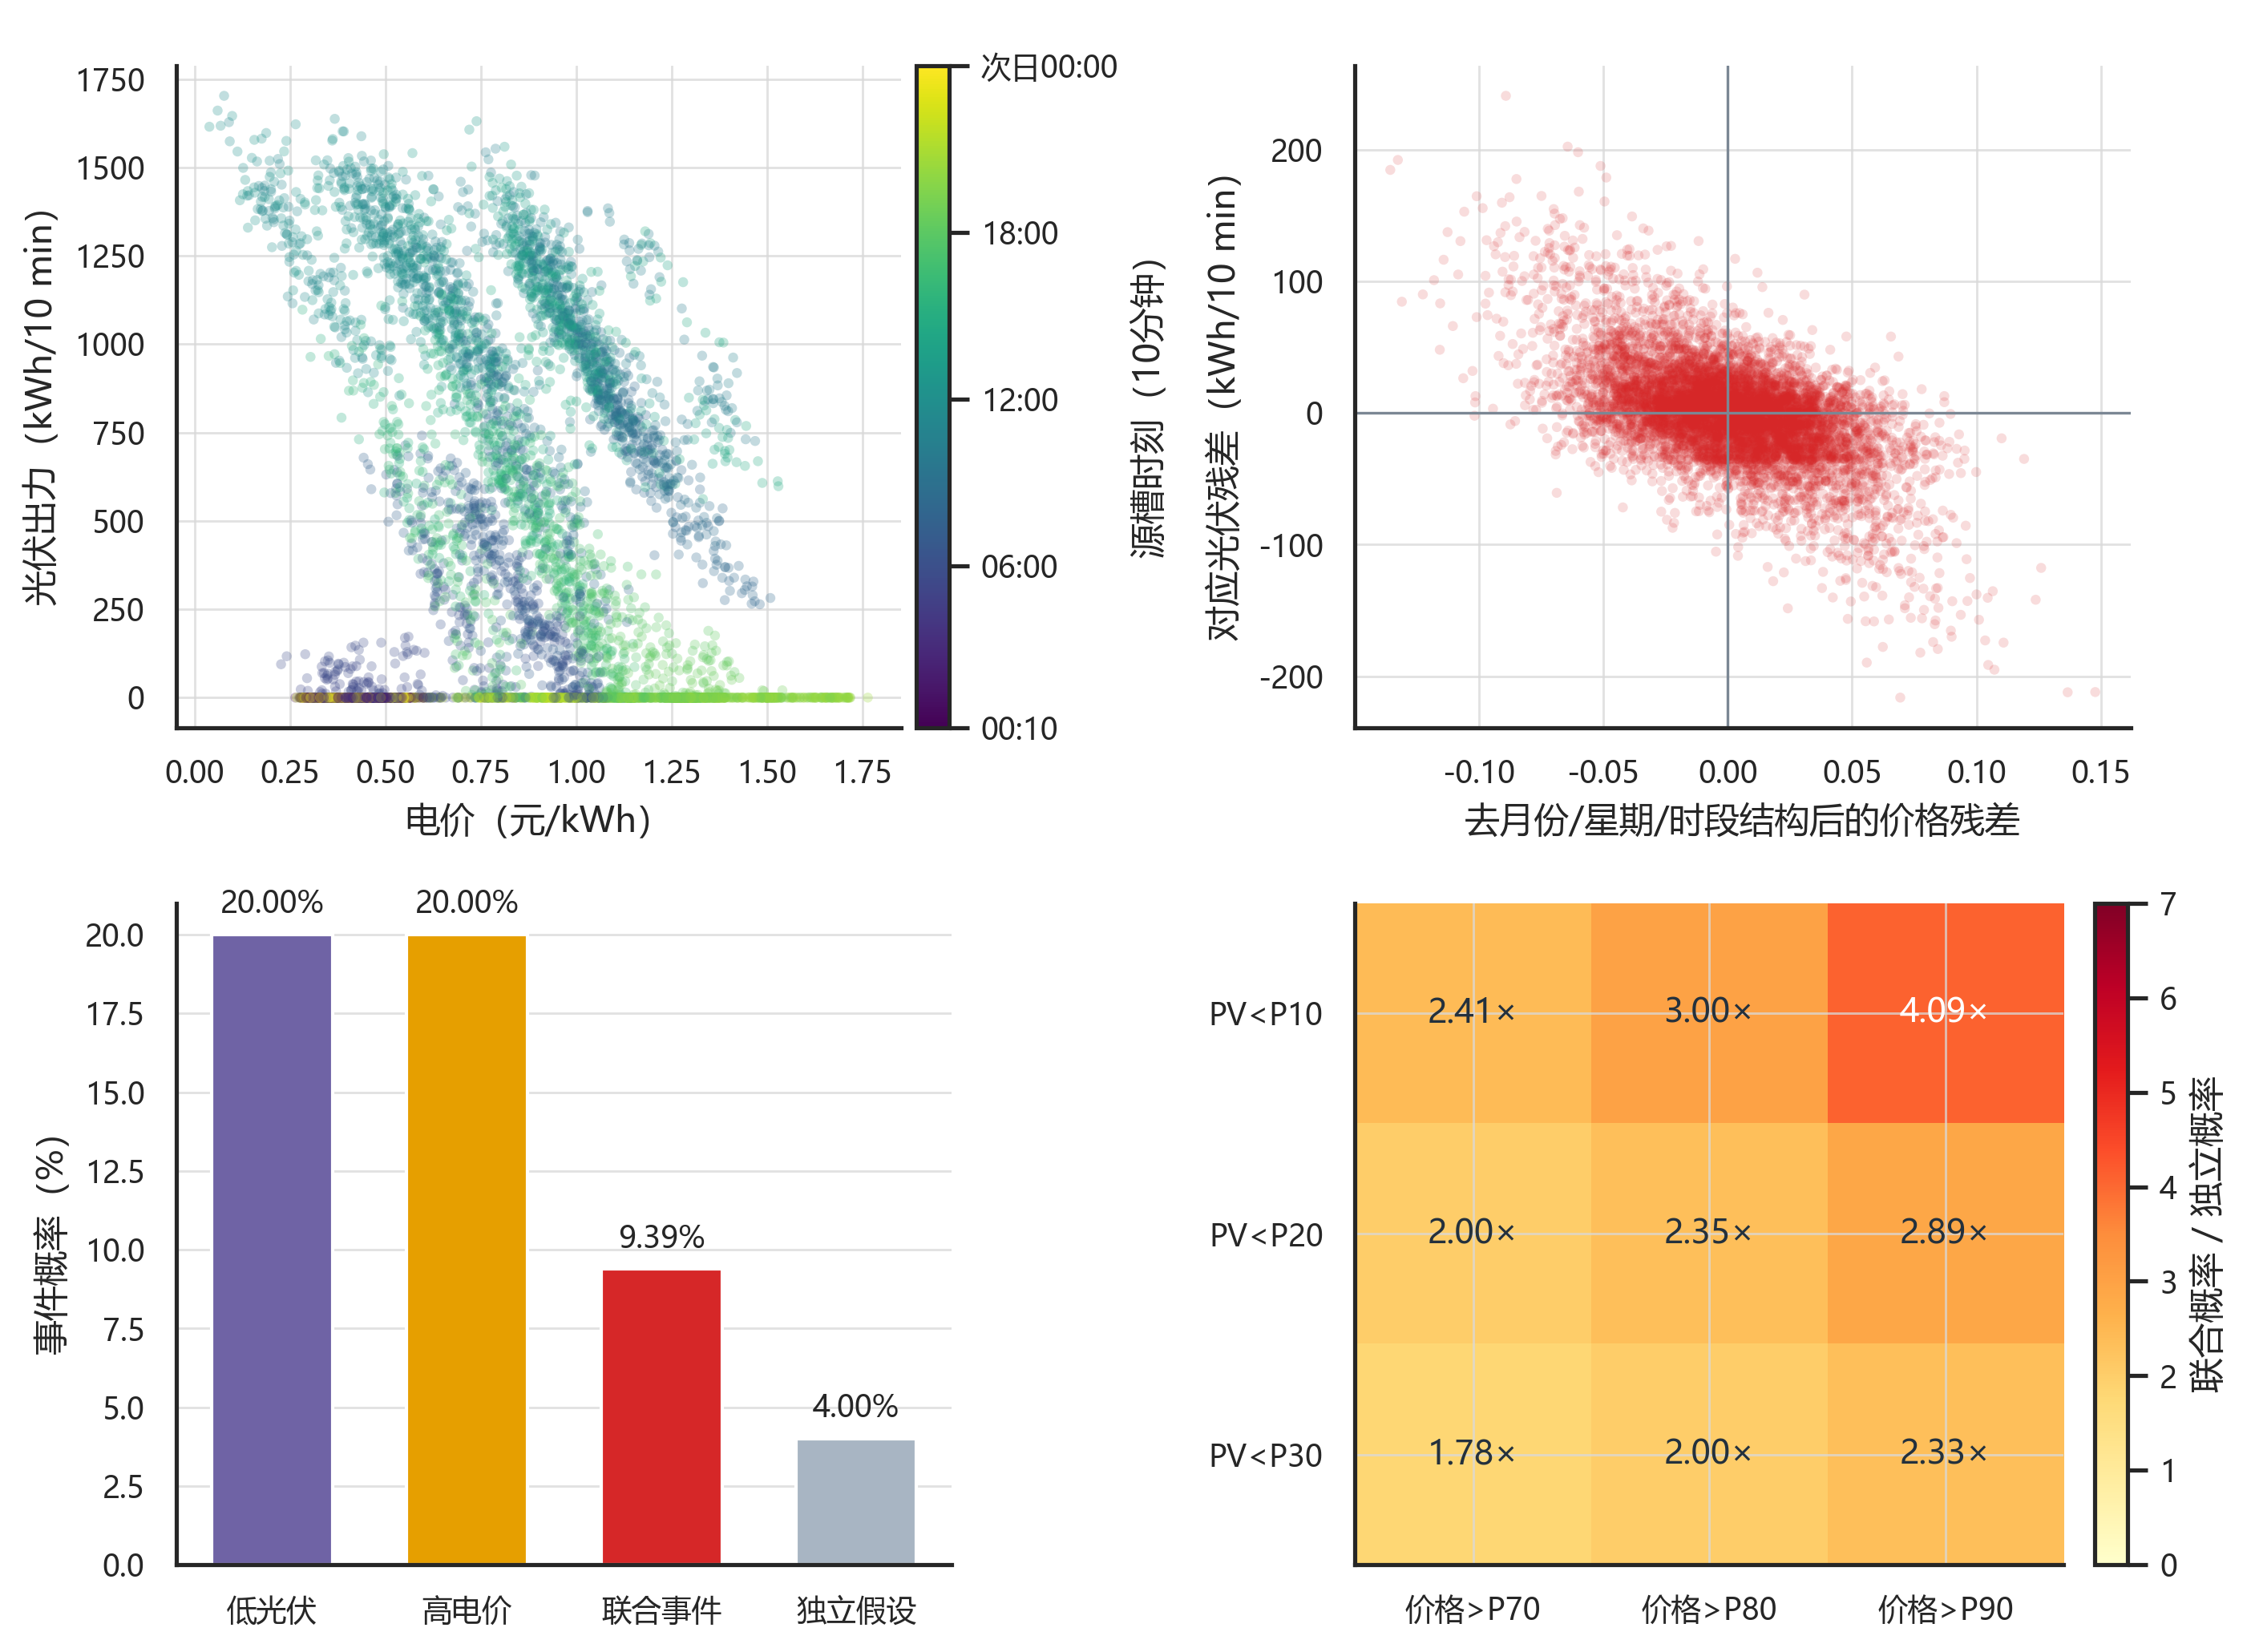
\includegraphics[width=\textwidth]{./figures/Q4_F04_光伏电价联合风险.png}
    \caption{光伏-电价联合风险图}
    \label{fig:q4-joint-risk}
\end{figure}


\subsection{模型建立}

\subsubsection{因果电价预测与决策价格}

价格预测误差由历史残差曲线描述。在每个发布时刻 \(r\in\{0,6,12,18\}\)，先由 Fourier 岭回归加最近 4 个同星期日曲线（权重 0.30）校正得到因果点预测 \(\hat p_{r,t}\)。正式模型直接取决策价格为
\begin{equation}
    p^{\mathrm{dec}}_{r,t}=\hat p_{r,t},
\end{equation}
即不额外叠加风险溢价；价格风险通过下文的配对 PV--价格场景与 CVaR 刻画。上分位风险溢价
\begin{equation}
    p^{\mathrm{dec}}_{r,t}=\max\Bigl(0,\;\hat p_{r,t}+w_r\bigl[Q_{q_r}(p^{\mathrm{hist}}_t-\hat p_{r,t})\bigr]^+\Bigr),
\end{equation}
其中 \(q=(0.925,0.900,0.925,0.900)\)，\(w=(1.00,1.25,1.00,1.00)\)，仅作为表 \ref{tab:q4-ablation-2}、\ref{tab:q4-ablation-3} 中“加入价格上分位风险溢价（对照）”方案的参数，由严格因果回测校准。

\subsubsection{联合光伏--电价场景}

设同一历史规划原点 \(h\) 得到的光伏误差块为 \(\boldsymbol{\varepsilon}^{PV}_h\)、电价误差块为 \(\boldsymbol{\varepsilon}^{p}_h\)。本文按历史日一一配对构造联合误差块 \((\boldsymbol{\varepsilon}^{PV}_h,\boldsymbol{\varepsilon}^{p}_h)\)，再压缩为不超过 12 组场景。由于价格残差与光伏短缺存在关联，历史分位数优先从光伏短缺最大的 30\% 样本中计算，样本不足时退化为全部历史误差。最终加入低光伏/高价格压力场景，概率取 0.10，其余场景概率等比例缩放。

\subsubsection{波动电价下的三日风险日前计划}

每天 0:00 用同一信息原点预测当天及未来最多两日的光伏与价格，建立连续三日风险 LP，仅锁定当日计划购电量 \(P_t\)。目标函数为
\begin{equation}
    \min\; C_{\rm plan}^{\rm point}+E[C_{\rm future}^{\rm point}]+E[C_{\rm emergency}]+\lambda\cdot\mathrm{CVaR}_{0.90}(C_{\rm emergency})+C_{\rm terminal},
\end{equation}
其中 \(C^{\rm point}\) 表示使用因果点预测电价的费用，紧急购电成本在联合 PV--价格场景上求期望与 CVaR。日内每 10 分钟获得真实光伏与真实电价后，仅执行当前时段储能充放电与紧急购电，重新求解剩余量。最终费用按附件 4 真实电价重算。

\subsubsection{波动电价下的四阶段调整}

00:00 日前计划给出 \(P_t\)。06:00、12:00、18:00 同步更新光伏与电价预测：电价先得到 24 个一小时均价，再按附件源标签映射到 144 个 10 分钟模块。对未发生时段重新优化最终购电量 \(A_t\)，已发生时段保持不变。主结算口径为
\begin{equation}
    C_t^{\rm normal}=p_t\min(P_t,A_t)+0.5p_t(P_t-A_t)^++1.5p_t(A_t-P_t)^+.
\end{equation}
10 分钟执行层在每个时段初使用已展示的真实电价与光伏，求解剩余时段 MPC。

\subsection{模型求解与结果分析}

\subsubsection{全年结果}

运行上述框架，得到 2025 年 2 月 1 日至 12 月 31 日共 334 天的结果，如表 \ref{tab:q4-annual} 所示。
\begin{table}[H]
    \centering
    \caption{问题四重做问题二与问题三全年运行结果对比}
    \label{tab:q4-annual}
    \small
    \begin{tabularx}{\textwidth}{CCC}
        \toprule
        指标 & 问题二 & 问题三 \\
        \midrule
        天数
            & 334
            & 334 \\

        实际结算计划费用
            & 13,515,807.04 元
            & 13,867,834.09 元 \\

        点预测/决策计划费用
            & 13,420,214.70 元
            & 13,697,522.15 元 \\

        基础结算费
            & --
            & 13,397,089.59 元 \\

        调整偏差费用
            & --
            & 832,669.25 元 \\

        主结算正常费用
            & --
            & 14,229,758.85 元 \\

        紧急购电费用
            & 1,743,379.36 元
            & 405,847.17 元 \\

        总购电费用
            & 15,259,186.40 元
            & 14,635,606.02 元 \\

        紧急购电量
            & 339,672.51 kWh
            & 92,397.77 kWh \\

        紧急购电天数
            & 310 天
            & 303 天 \\

        弃光量
            & 2,326,399.06 kWh
            & 1,249,954.24 kWh \\

        未利用计划购电量
            & --
            & 705,802.07 kWh \\

        最大平衡误差
            & 0.000000 kWh
            & 0.000000 kWh \\

        同时充放电时段
            & 0
            & 0 \\

        \bottomrule
    \end{tabularx}
\end{table}



与问题四-2 相比，问题四-3 引入日内光伏与电价同步更新后，全年总费用降低 623,580.38 元（$-4.09\%$），紧急购电量降低 247,274.74 kWh（$-72.80\%$），紧急购电费降低 1,337,532.19 元（$-76.72\%$）；产生约 83.27 万元的调整策略费用，说明更新把高价紧急购电转化为低价计划调整以降低总成本。

图 \ref{fig:q4-cost-composition} 进一步展示了这一风险转移机制：问题四-2 的日前计划在面对不可预知的电价波动时，被迫依赖高倍数的紧急购电（红色部分），导致总费用高达 15.26 百万元；问题四-3 通过 06:00/12:00/18:00 的同步更新，将大量本需以高价紧急购电弥补的缺口提前转化为计划内的合同调整（黄色部分），虽然产生了约 83 万元的调整费，但紧急购电费从 174.34 万元降至 40.58 万元，最终总费用降至 14.64 百万元。

\begin{figure}[H]
    \centering
    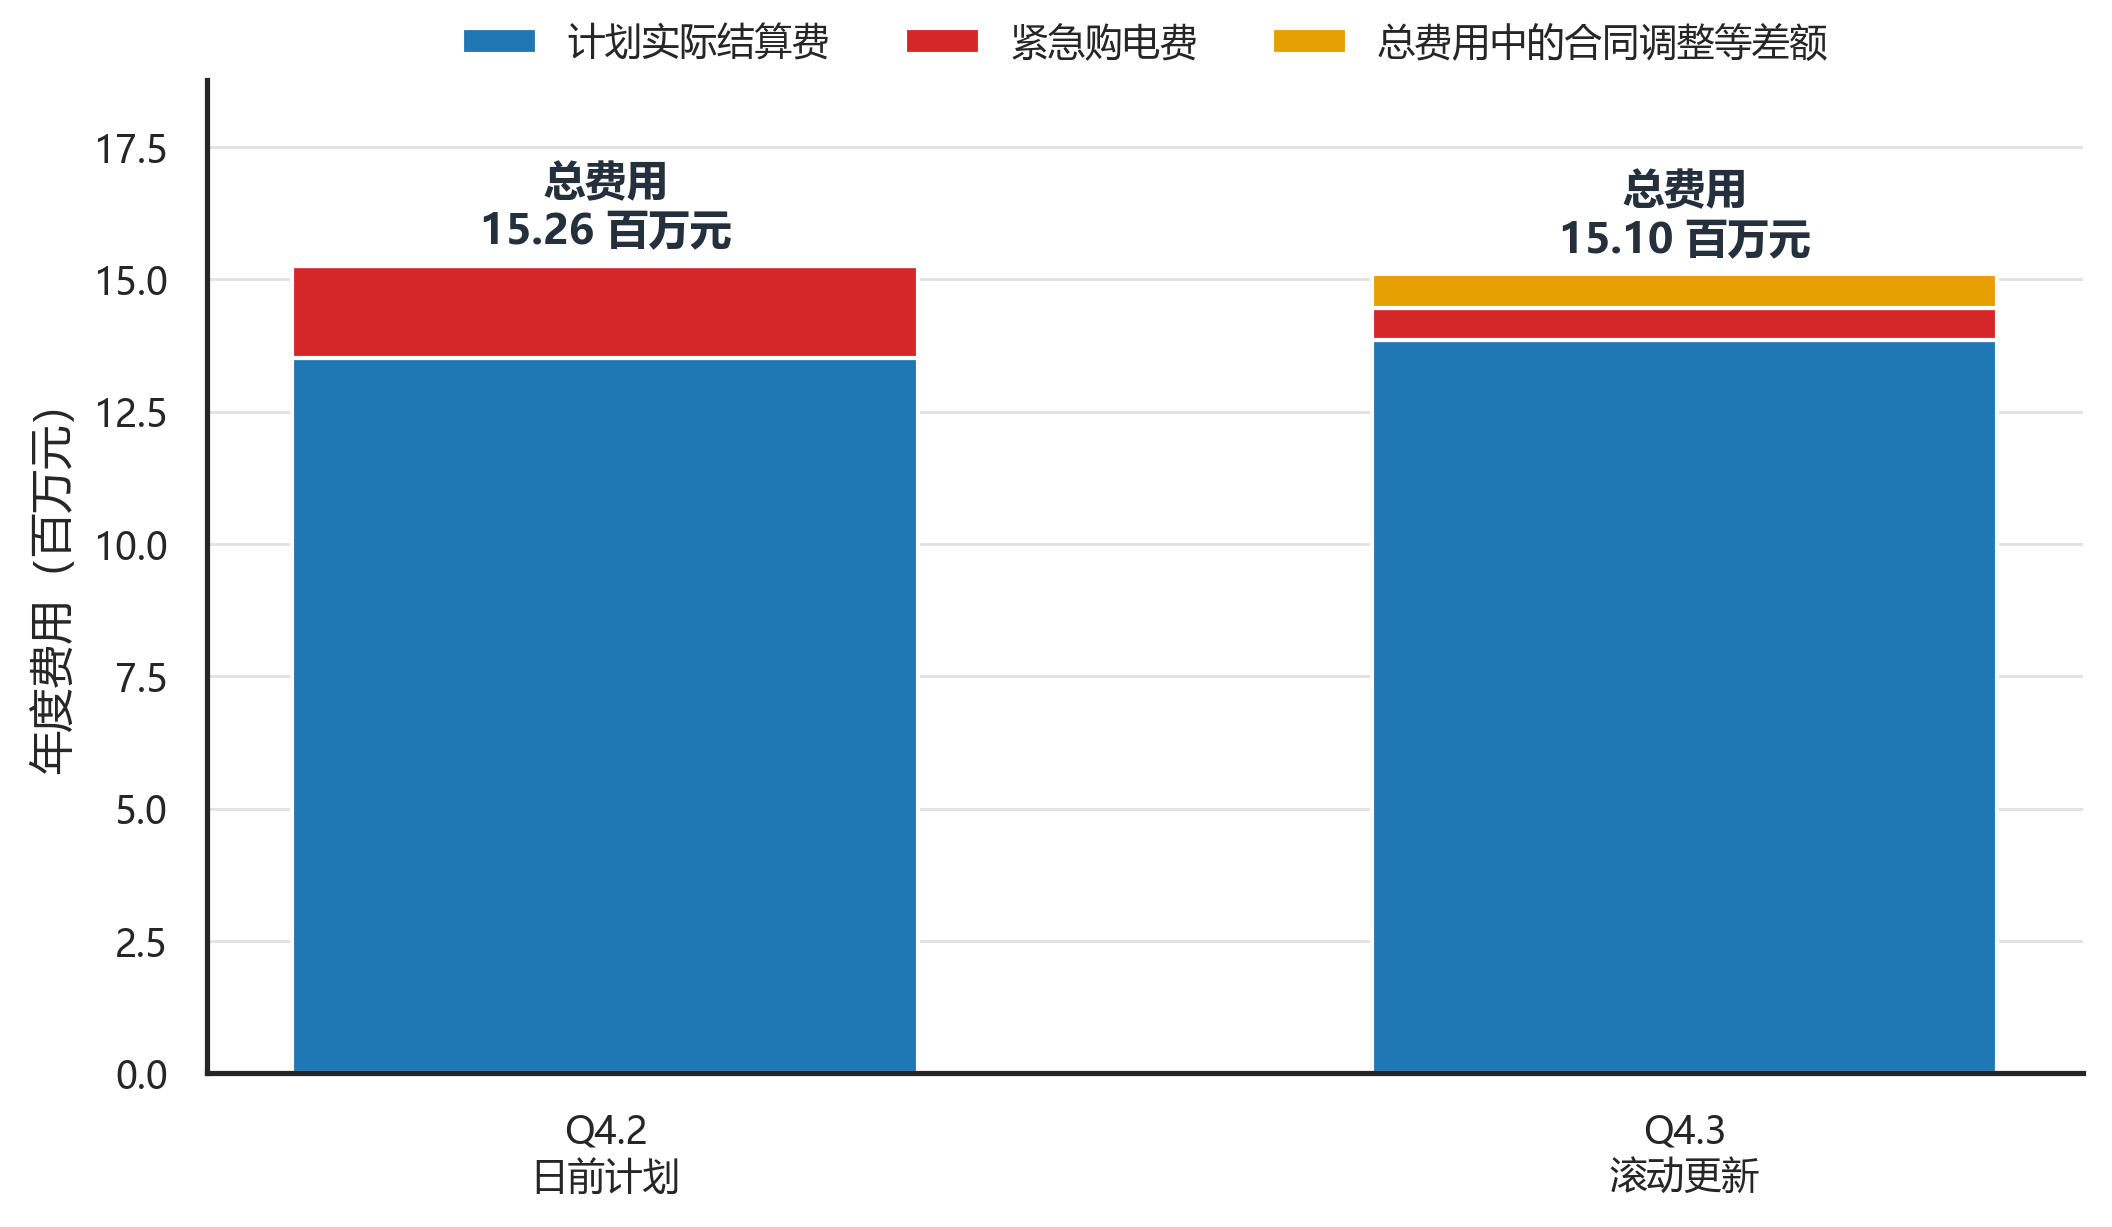
\includegraphics[width=0.6\textwidth]{./figures/Q4_F01_费用构成与风险转移.png}
    \caption{日内更新的高倍数紧急购电费用转化效应}
    \label{fig:q4-cost-composition}
\end{figure}

\subsubsection{指定日期紧急购电分析}

\textbf{3 月 20 日、6 月 21 日、9 月 23 日、12 月 21 日的费用见附录表 \ref{tab:app-q4-2-settlement} 和表 \ref{tab:app-q4-3-settlement}，主要紧急购电区间见附录表 \ref{tab:app-q4-2-emergency} 和表 \ref{tab:app-q4-3-emergency}。}


上述全年统计与指定日结果由“未来信息”与“已执行合同”的严格区分所保障。以代表日 2025-07-18 为例，图 \ref{fig:q4-mpc-day} 上半部分显示，随着 06:00、12:00、18:00 不断释放新价格信息，各发布时刻的价格预测逐步向实际电价收敛；中间子图显示日前计划购电量（蓝色）在已执行区间保持不变，而未执行区间则根据更新后的预测与 SOC 状态不断调整（紫色），紧急购电（橙色）仅在实际出现缺口时被调用；下半部分 SOC 曲线显示储能在光伏富余、电价较低的午间充电，在电价较高的傍晚放电，体现了 MPC 执行层对因果约束的遵守——即已执行策略不受未来扰动影响。

\begin{figure}[H]
    \centering
    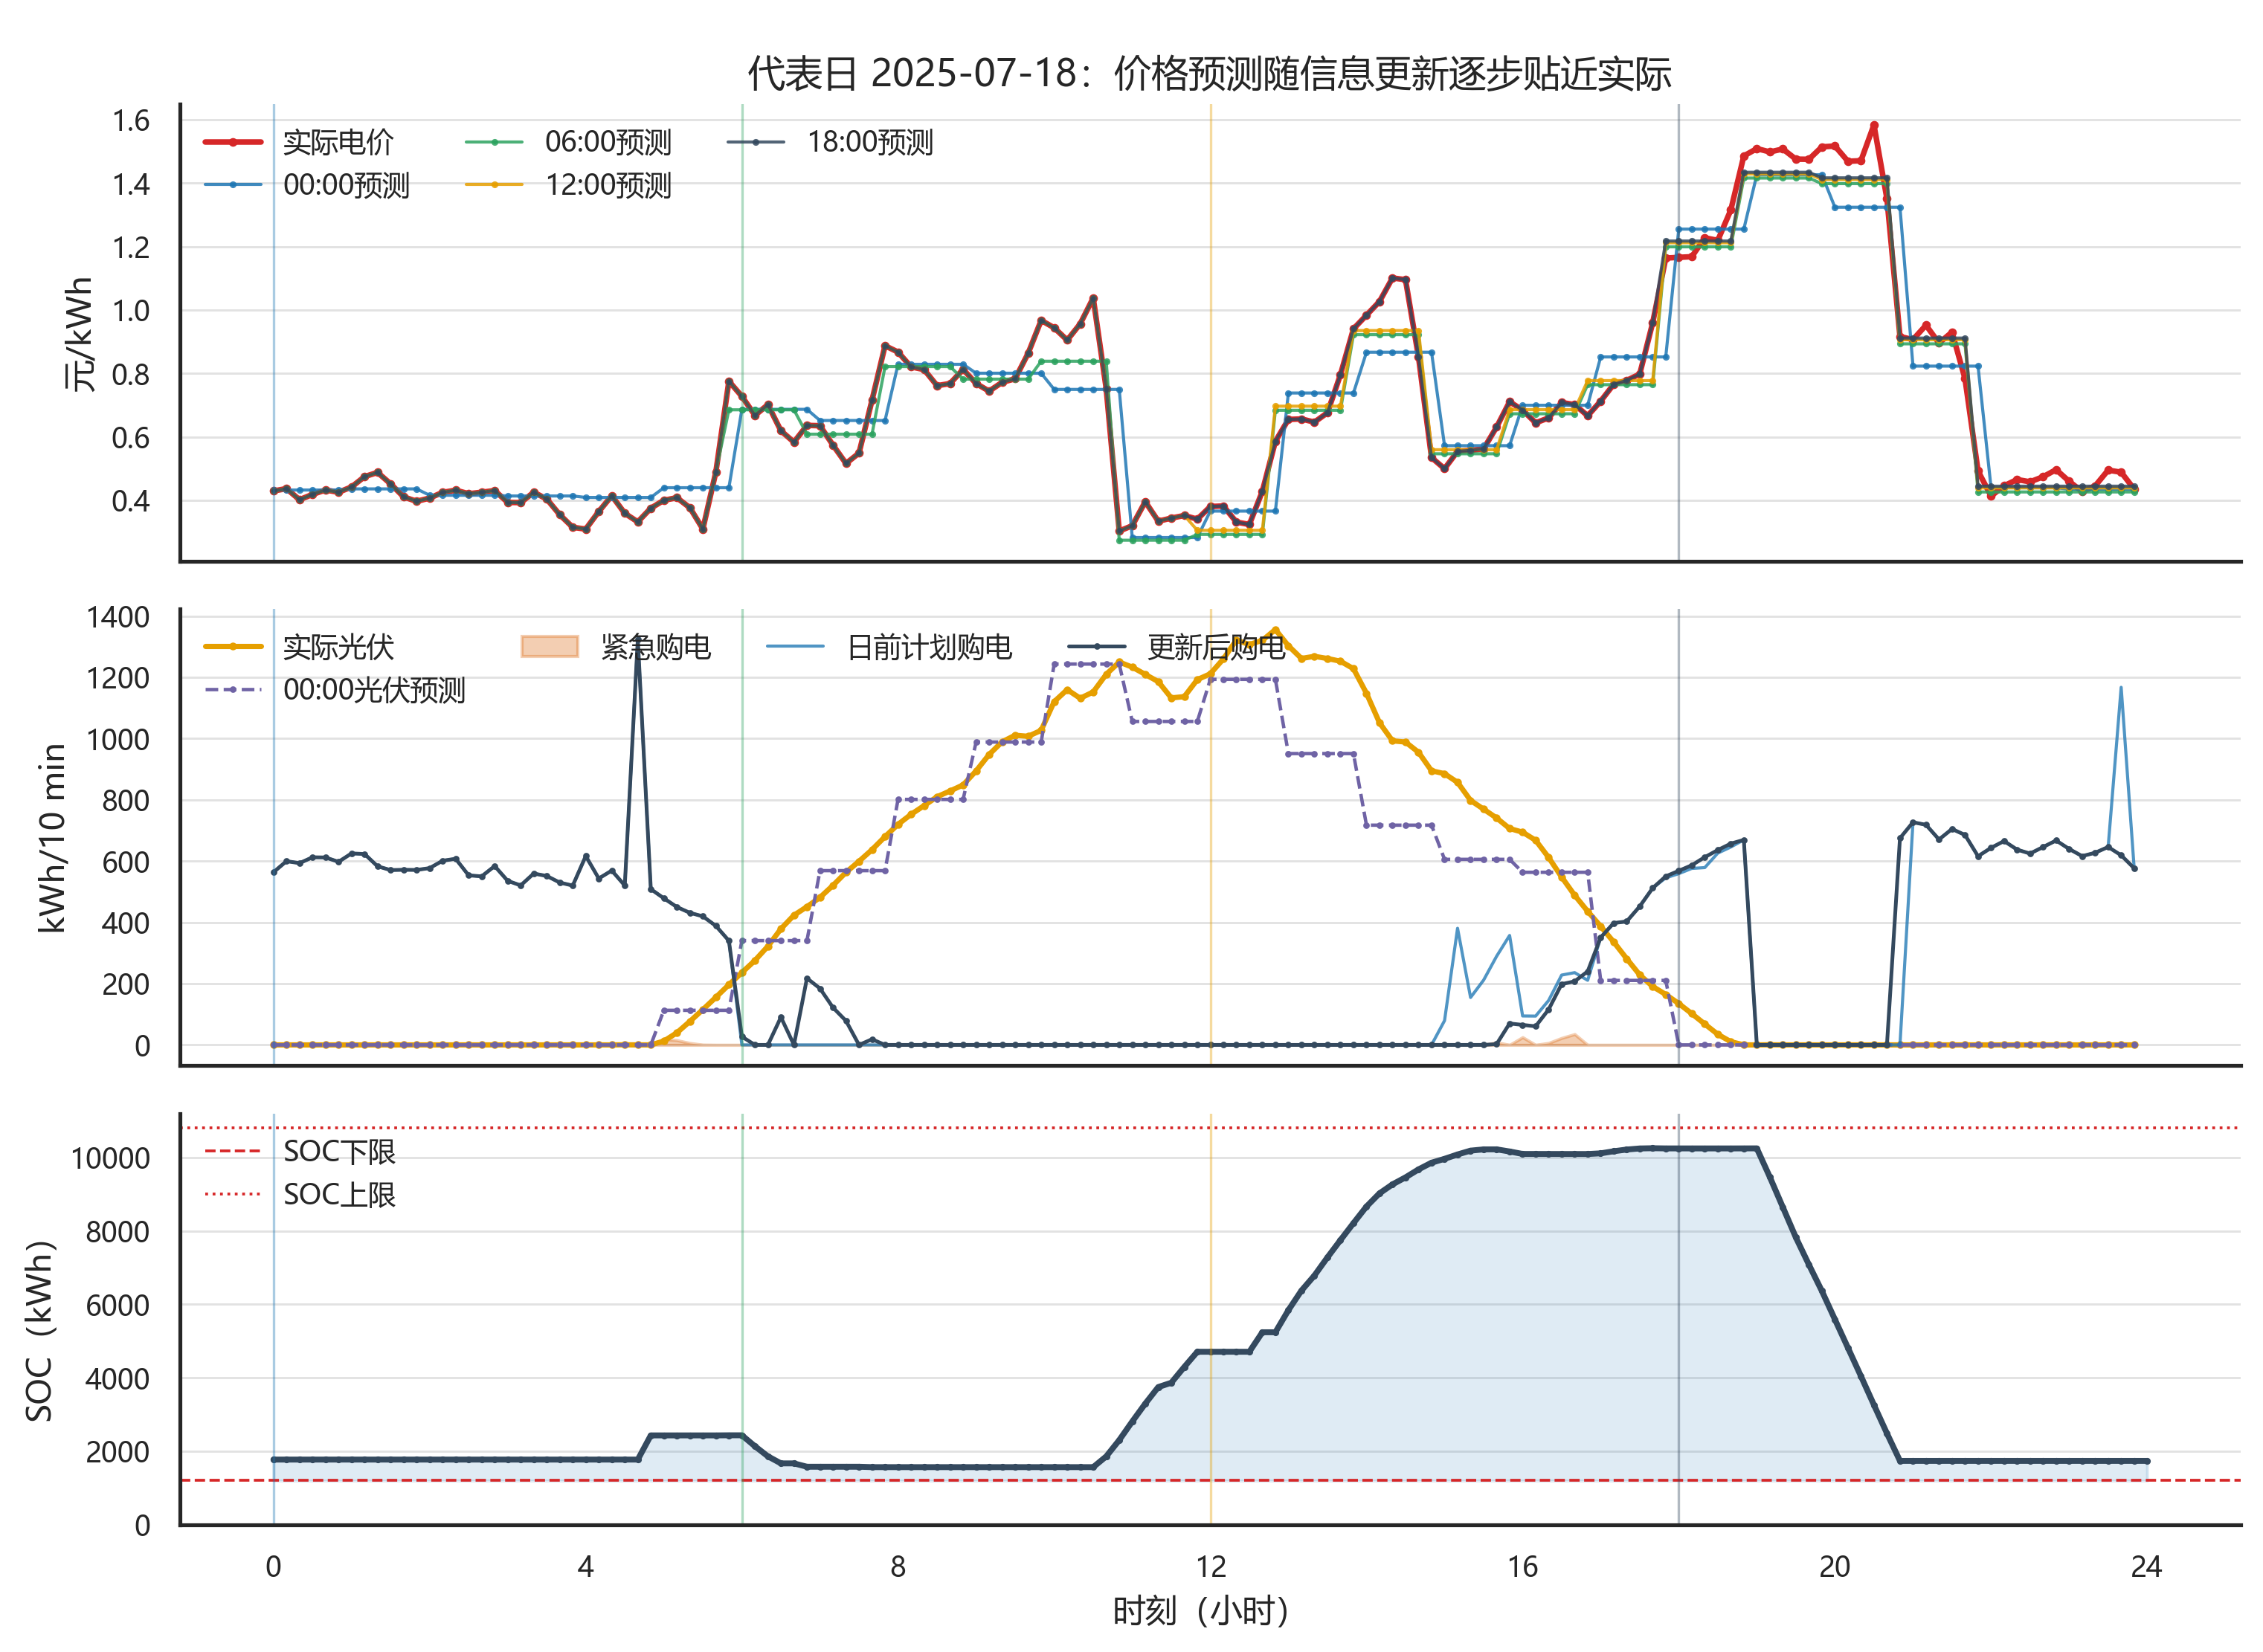
\includegraphics[width=0.6\textwidth]{./figures/Q4_F05_代表日滚动控制.png}
    \caption{问题四 MPC 执行层}
    \label{fig:q4-mpc-day}
\end{figure}

其他必要结果已保存到 result4-2.xlsx及 result4-3.xlsx。
\subsection{模型检验}

\subsubsection{价格预测精度与风险参数说明}

价格预测采用 Fourier 岭回归加最近 4 个同星期日曲线（权重 0.30）校正。生产模型在全年 q4 输出窗口的日曲线 MAE 为 0.0417 元/kWh，优于季节性朴素基准 0.0472 元/kWh；各发布时刻未来区间 MAE 见表 \ref{tab:q4-price-forecast}。

\begin{table}[H]
    \centering
    \caption{生产模型价格预测误差（元/kWh）}
    \label{tab:q4-price-forecast}
    \begin{tabularx}{\textwidth}{CCCCC}
        \toprule
        指标 & 0:00 & 6:00 & 12:00 & 18:00 \\
        \midrule
        未来 MAE & 0.0724 & 0.0533 & 0.0506 & 0.0475 \\
        未来 RMSE & 0.1097 & 0.0704 & 0.0665 & 0.0636 \\
        \bottomrule
    \end{tabularx}
\end{table}

需要说明的是上分位风险溢价参数 \(q=(0.925,0.900,0.925,0.900)\)、\(w=(1.00,1.25,1.00,1.00)\) 由严格因果回测校准，但仅在消融对照方案“加入价格上分位风险溢价（对照）”中使用；正式结果的风险由配对 PV--价格场景与 CVaR 决定。

\subsubsection{策略消融与联合场景必要性}

在固定初始 SOC 的代表日（2025-07-18）上进行对照，结果见表 \ref{tab:q4-ablation-2} 与表 \ref{tab:q4-ablation-3}。

\begin{table}[H]
  \centering
  \caption{问题四-2 代表日策略消融}
  \label{tab:q4-ablation-2}
  \small
  \begin{tabularx}{\textwidth}{p{0.25\textwidth}cccc}
    \toprule
    方案 & 计划实际结算费（元） & 紧急购电费（元） & 总费用（元） & 紧急电量（kWh） \\
    \midrule
    生产模型 & 22,401.00 & 15,218.52 & 37,619.52 & 2,356.55 \\
    加入价格上分位风险溢价 & 22,397.93 & 15,349.97 & 37,747.90 & 2,358.04 \\
    去除 PV--价格联合场景 & 22,388.53 & 2,172.58 & 24,561.11 & 529.83 \\
    价格完美信息参考方案 & 22,249.56 & 2,359.35 & 24,608.91 & 644.06 \\
    \bottomrule
  \end{tabularx}
\end{table}

\begin{table}[H]
  \centering
  \caption{问题四-3 代表日策略消融}
  \label{tab:q4-ablation-3}
  \small
  \begin{tabularx}{\textwidth}{p{0.25\textwidth}cccc}
    \toprule
    方案 & 计划实际结算费（元） & 紧急购电费（元） & 总费用（元） & 紧急电量（kWh） \\
    \midrule
    生产模型 & 24,059.52 & 144.40 & 25,221.23 & 50.84 \\
    加入价格上分位风险溢价 & 24,754.56 & 125.70 & 24,880.25 & 34.33 \\
    去除 PV--价格联合场景 & 25,679.44 & 27.40 & 25,706.85 & 8.01 \\
    价格完美信息参考方案 & 25,214.71 & 47.35 & 25,262.05 & 14.60 \\
    取消日内更新（仅 00:00） & 24,059.52 & 302.57 & 24,362.09 & 96.50 \\
    \bottomrule
  \end{tabularx}
\end{table}

表 \ref{tab:q4-ablation-2} 显示，去除 PV--价格联合场景后代表日总费用显著下降，说明独立误差场景低估了光伏短缺与高价并发的尾部风险；生产模型通过配对场景保留该风险，紧急购电费更高但更贴近实际。表 \ref{tab:q4-ablation-3} 中，取消日内更新使该代表日总费用下降 859.14 元，但紧急购电量增加至 96.50 kWh，说明日内更新能够降低紧急供电风险，但不保证单个代表日的总费用必然下降，说明同步电价--光伏更新具有明显价值。

\section{模型评价与推广}

\subsection{模型优点}

\begin{enumerate}
    \item \textbf{多时间尺度框架完整，经济性改善显著：}
    
    \hspace{2em}本文从问题一的确定性日前优化出发，到问题二的三日滚动随机规划、问题三的日内多阶段调整，再到问题四的波动电价四阶段同步更新，逐步递进，形成“日前计划—日内调整—实时执行”的完整决策链条。四个问题共用能量平衡、储能 SOC 递推、充放电约束等基础模块，又根据风险来源的差异接续引入滚动更新、联合场景、CVaR 等增量机制，与此同时带来了显著的经济改善：问题三引入日内四次更新后，全年紧急购电量较问题二下降约 61.63\%（总费用因调整偏差结算上升约 1.39\%）；问题四中，问题四-3 相比问题四-2 的总费用下降 4.09\%，紧急购电量下降 72.80\%。这些结果表明，模型通过增加调整结算费用换取了紧急购电风险下降。

    \item \textbf{因果性约束严：}
    
    \hspace{2em}针对光伏预测、电价预测、误差场景生成，本文均采用了\textbf{严格因果回测}：预测模型只使用目标时刻之前的历史数据，场景从历史残差中抽样，日内 MPC 只根据当前及已揭示信息做决策。

    \item \textbf{风险刻画贴近实际运行：}
    
    不论是题二、三通过历史预报误差生成连续多日场景并叠加低光伏压力场景，还是问题四发现 PV 与电价原始序列弱相关但去结构后残差显著负相关，从而生成联合 PV--价格场景并加入低光伏/高价格压力场景，都\textbf{规避了独立误差场景低估“光伏短缺同时电价高企”的尾部风险}，比简单叠加风险溢价更符合实际电力市场特征。
\end{enumerate}


\subsection{模型缺点}

\begin{enumerate}
    \item \textbf{小区负载被视为已知序列：}
    
    \hspace{2em}本文四个问题均将小区负载作为已知输入，未对其进行预测或作为随机变量处理。然而实际运行中，小区负载会随当日天气、用户行为、突发事件等因素实时变化，会直接影响购电计划的可执行性与经济性。

    \item \textbf{历史平稳性假设带来不确定性：}
    
    \hspace{2em}为简化处理，本文的场景生成和 CVaR 参数校准均基于“未来误差分布与历史一致”的假设。当目标年出现极端天气、电价机制调整或负荷结构突变时，历史残差可能无法代表当日及未来风险，导致风险评估偏离实际。

    \item \textbf{场景压缩存在信息损失：}
    
    \hspace{2em}为控制计算规模，联合 PV--价格场景被压缩至不超过 12 组。损失了部分中间状态的概率细节，对中等强度风险事件的刻画不够精细。

    \item \textbf{未考虑网络与设备动态：}
    
    \hspace{2em}模型假设储能效率恒定、设备无衰减，未涉及线路容量、电池循环老化等因素。在实际工程应用中，这些约束可能影响计划的可执行性。
    
\end{enumerate}


\subsection{模型推广}

本文的微网购电优化框架可进一步向多维度拓展。新能源方面，将光伏扩展为风--光--储--荷多能互补系统，将风电出力、电动汽车充电负荷等新的不确定性源纳入联合场景，可研究多能协同优化。宏观电力市场方面，将单一微网扩展为多个互联微网或虚拟电厂，引入 peer-to-peer 交易\textsuperscript{[8]}、实时电价、需求响应等机制，可研究微网群之间的能量共享与动态价格设定。






\newpage
%参考文献


\begin{thebibliography}{99}
\bibitem{1} Huangfu Q, Hall J A J. Parallelizing the dual revised simplex method[J]. Mathematical Programming Computation, 2018, 10(1): 119-142.
\bibitem{2} Hoerl A E, Kennard R W. Ridge regression: Biased estimation for nonorthogonal problems[J]. Technometrics, 1970, 12(1): 55-67; Harvey A C. Forecasting, structural time series models and the Kalman filter[M]. Cambridge University Press, 1989.
\bibitem{3} Dupa\v{c}ov\'a J, Gr\"owe-Kuska N, R\"omisch W. Scenario reduction in stochastic programming: An approach using probability metrics[J]. Mathematical Programming, 2003, 95(3): 493-511.
\bibitem{4} Rockafellar R T, Uryasev S. Optimization of conditional value-at-risk[J]. Journal of Risk, 2000, 2(3): 21-41.
\bibitem{5} Ben-Tal A, El Ghaoui L, Nemirovski A. Robust optimization[M]. Princeton University Press, 2009.
\bibitem{6} Koenker R, Bassett G. Regression quantiles[J]. Econometrica, 1978, 46(1): 33-50; Gneiting T, Balabdaoui F, Raftery A E. Probabilistic forecasts, calibration and sharpness[J]. Journal of the Royal Statistical Society: Series B, 2007, 69(2): 243-268.
\bibitem{7} Hintze J L, Nelson R D. Violin plots: A box plot-density trace synergism[J]. The American Statistician, 1998, 52(2): 181-184.
\bibitem{8} Sousa T, Soares T, Pinson P, Moret F, Baroche T, Sorin E. Peer-to-peer and community-based markets: A comprehensive review[J]. Renewable and Sustainable Energy Reviews, 2019, 104: 367-378.
\end{thebibliography}


\newpage




%附录

\begin{appendices}

% 四个问题结果表附录：在主文档 appendix 之后用 input{问题一至四附录表格.tex} 插入。
% 数据来源：C题/结果下当前正式结果文件；数值统一保留四位小数。
% 主文档导言区需加载：booktabs、longtable、array。

% 四个问题结果表附录：在主文档 appendix 之后用 input{问题一至四附录表格.tex} 插入。
% 数据来源：C题/结果下当前正式结果文件；数值统一保留四位小数。
% 主文档导言区需加载：booktabs、longtable、array。

\begingroup
\small
\setlength{\tabcolsep}{3.5pt}
\renewcommand{\arraystretch}{1.08}
\setlength{\LTpre}{2pt}
\setlength{\LTpost}{4pt}
\setlength{\abovecaptionskip}{3pt}
\setlength{\belowcaptionskip}{2pt}

\section{问题一至问题四结果表}
\noindent 本附录列出题目要求的指定时段和指定日期；全年 10 分钟完整策略保存在题目规定的 result 文件中。电量单位为 kWh，费用单位为元；时间段采用左闭右开记法。
\subsection{问题一：附件 1 示例日}
\noindent 问题一的输入为附件 1 的单日价格、负荷和光伏预测，因此不对应自然日期。
\begingroup
\footnotesize
\begin{longtable}{@{}l r@{\hspace{8pt}}l r@{\hspace{8pt}}l r@{}}
\caption{问题一指定时段计划购电量及全天合计、购电费}\label{tab:app-q1-plan}\\
\toprule
\multicolumn{6}{c}{\textbf{指定时段计划购电量}}\\
\textbf{时间段} & \textbf{购电量} & \textbf{时间段} & \textbf{购电量} & \textbf{时间段} & \textbf{购电量}\\
\midrule
\endfirsthead
\caption[]{问题一指定时段计划购电量及全天合计、购电费（续）}\\
\toprule
\multicolumn{6}{c}{\textbf{指定时段计划购电量}}\\
\textbf{时间段} & \textbf{购电量} & \textbf{时间段} & \textbf{购电量} & \textbf{时间段} & \textbf{购电量}\\
\midrule
\endhead
\midrule
\multicolumn{6}{r@{}}{\footnotesize 续下页}\\
\endfoot
\bottomrule
\endlastfoot
\multicolumn{6}{l}{\textbf{日期：附件1示例日}\hfill\textit{指定时段购电}}\\
\noalign{\penalty 10000}
\cmidrule(lr){1-6}
\texttt{10:00--10:10} & 0.0000 & \texttt{12:00--12:10} & 486.4029 & \texttt{14:00--14:10} & 0.0000\\
\noalign{\penalty 10000}
\texttt{16:00--16:10} & 394.9315 & \texttt{18:00--18:10} & 636.9826 & \texttt{20:00--20:10} & 0.0000\\
\noalign{\penalty 10000}
\addlinespace[1pt]
\cmidrule(lr){1-3}\cmidrule(lr){4-6}
\multicolumn{2}{l}{\textbf{全天购电量}} & \textbf{59\,482.6990} & \multicolumn{2}{l}{\textbf{全天购电费}} & \textbf{35\,126.9486}\\
\end{longtable}
\endgroup
\begingroup
\footnotesize
\begin{longtable}{@{}p{5.2cm} r r@{}}
\caption{问题一指定时段四小时充放电量及首末储电量}\label{tab:app-q1-storage}\\
\toprule
\multicolumn{3}{c}{\textbf{四小时充放电量}}\\
\multicolumn{3}{c}{\textbf{日期：附件1示例日}}\\
\textbf{时间段} & \textbf{充电量} & \textbf{放电量}\\
\midrule
\endfirsthead
\caption[]{问题一指定时段四小时充放电量及首末储电量（续）}\\
\toprule
\multicolumn{3}{c}{\textbf{日期：附件1示例日}}\\
\textbf{时间段} & \textbf{充电量} & \textbf{放电量}\\
\midrule
\endhead
\midrule
\multicolumn{3}{r@{}}{\footnotesize 续下页}\\
\endfoot
\bottomrule
\endlastfoot
\texttt{0:00--4:00} & 4\,500.0000 & 0.0000\\
\texttt{4:00--8:00} & 833.3333 & 6\,365.8412\\
\texttt{8:00--12:00} & 4\,787.9643 & 1\,702.9970\\
\texttt{12:00--16:00} & 5\,286.0352 & 91.1014\\
\texttt{16:00--20:00} & 0.0000 & 5\,780.1319\\
\texttt{20:00--24:00} & 5\,333.3333 & 2\,859.8681\\
\addlinespace[1pt]
\cmidrule(lr){1-3}
\multicolumn{2}{l}{\textbf{日初 SOC}} & \textbf{6\,000.0000}\\
\multicolumn{2}{l}{\textbf{日末 SOC}} & \textbf{6\,000.0000}\\
\end{longtable}
\endgroup
\noindent\footnotesize 注：问题一首末储电量均为 6000.0000 kWh，符合题目要求。
\normalsize

\subsection{问题二：固定电价下四个指定日期}
\noindent 以下表格分别对应题目表 1、表 2 和表 3；日期分组行将不同指标明确分开。
\begingroup
\footnotesize
\begin{longtable}{@{}l r@{\hspace{8pt}}l r@{\hspace{8pt}}l r@{}}
\caption{问题二指定时段计划购电量及全天合计、购电费}\label{tab:app-q2-plan}\\
\toprule
\multicolumn{6}{c}{\textbf{指定时段计划购电量}}\\
\textbf{时间段} & \textbf{购电量} & \textbf{时间段} & \textbf{购电量} & \textbf{时间段} & \textbf{购电量}\\
\midrule
\endfirsthead
\caption[]{问题二指定时段计划购电量及全天合计、购电费（续）}\\
\toprule
\multicolumn{6}{c}{\textbf{指定时段计划购电量}}\\
\textbf{时间段} & \textbf{购电量} & \textbf{时间段} & \textbf{购电量} & \textbf{时间段} & \textbf{购电量}\\
\midrule
\endhead
\midrule
\multicolumn{6}{r@{}}{\footnotesize 续下页}\\
\endfoot
\bottomrule
\endlastfoot
\multicolumn{6}{l}{\textbf{日期：2025-03-20}\hfill\textit{指定时段购电}}\\
\noalign{\penalty 10000}
\cmidrule(lr){1-6}
\texttt{10:00--10:10} & 0.0000 & \texttt{12:00--12:10} & 674.8010 & \texttt{14:00--14:10} & 0.0000\\
\noalign{\penalty 10000}
\texttt{16:00--16:10} & 491.6659 & \texttt{18:00--18:10} & 682.3533 & \texttt{20:00--20:10} & 0.0000\\
\noalign{\penalty 10000}
\addlinespace[1pt]
\cmidrule(lr){1-3}\cmidrule(lr){4-6}
\multicolumn{2}{l}{\textbf{全天购电量}} & \textbf{64\,236.1943} & \multicolumn{2}{l}{\textbf{全天购电费}} & \textbf{40\,149.9148}\\
\addlinespace[2pt]\midrule
\multicolumn{6}{l}{\textbf{日期：2025-06-21}\hfill\textit{指定时段购电}}\\
\noalign{\penalty 10000}
\cmidrule(lr){1-6}
\texttt{10:00--10:10} & 0.0000 & \texttt{12:00--12:10} & 0.0000 & \texttt{14:00--14:10} & 0.0000\\
\noalign{\penalty 10000}
\texttt{16:00--16:10} & 112.5318 & \texttt{18:00--18:10} & 387.0929 & \texttt{20:00--20:10} & 0.0000\\
\noalign{\penalty 10000}
\addlinespace[1pt]
\cmidrule(lr){1-3}\cmidrule(lr){4-6}
\multicolumn{2}{l}{\textbf{全天购电量}} & \textbf{41\,031.0774} & \multicolumn{2}{l}{\textbf{全天购电费}} & \textbf{22\,192.8847}\\
\addlinespace[2pt]\midrule
\multicolumn{6}{l}{\textbf{日期：2025-09-23}\hfill\textit{指定时段购电}}\\
\noalign{\penalty 10000}
\cmidrule(lr){1-6}
\texttt{10:00--10:10} & 0.0000 & \texttt{12:00--12:10} & 508.1138 & \texttt{14:00--14:10} & 0.0000\\
\noalign{\penalty 10000}
\texttt{16:00--16:10} & 494.5129 & \texttt{18:00--18:10} & 715.7513 & \texttt{20:00--20:10} & 0.0000\\
\noalign{\penalty 10000}
\addlinespace[1pt]
\cmidrule(lr){1-3}\cmidrule(lr){4-6}
\multicolumn{2}{l}{\textbf{全天购电量}} & \textbf{67\,463.8476} & \multicolumn{2}{l}{\textbf{全天购电费}} & \textbf{41\,830.1200}\\
\addlinespace[2pt]\midrule
\multicolumn{6}{l}{\textbf{日期：2025-12-21}\hfill\textit{指定时段购电}}\\
\noalign{\penalty 10000}
\cmidrule(lr){1-6}
\texttt{10:00--10:10} & 0.0000 & \texttt{12:00--12:10} & 1\,006.1064 & \texttt{14:00--14:10} & 0.0000\\
\noalign{\penalty 10000}
\texttt{16:00--16:10} & 800.0563 & \texttt{18:00--18:10} & 694.7699 & \texttt{20:00--20:10} & 0.0000\\
\noalign{\penalty 10000}
\addlinespace[1pt]
\cmidrule(lr){1-3}\cmidrule(lr){4-6}
\multicolumn{2}{l}{\textbf{全天购电量}} & \textbf{96\,153.7242} & \multicolumn{2}{l}{\textbf{全天购电费}} & \textbf{62\,375.2035}\\
\end{longtable}
\endgroup

\begingroup
\footnotesize
\begin{longtable}{@{}p{3.2cm} r r@{\hspace{7pt}}p{3.2cm} r r@{}}
\caption{问题二指定时段四小时充放电量及首末储电量}\label{tab:app-q2-storage}\\
\toprule
\multicolumn{6}{c}{\textbf{四小时充放电量}}\\
\multicolumn{3}{c}{\textbf{日期：2025-03-20}} & \multicolumn{3}{c}{\textbf{日期：2025-06-21}}\\
\textbf{时间段} & \textbf{充电量} & \textbf{放电量} & \textbf{时间段} & \textbf{充电量} & \textbf{放电量}\\
\midrule
\endfirsthead
\caption[]{问题二指定时段四小时充放电量及首末储电量（续）}\\
\toprule
\multicolumn{3}{c}{\textbf{日期：2025-03-20}} & \multicolumn{3}{c}{\textbf{日期：2025-06-21}}\\
\textbf{时间段} & \textbf{充电量} & \textbf{放电量} & \textbf{时间段} & \textbf{充电量} & \textbf{放电量}\\
\midrule
\endhead
\midrule
\multicolumn{6}{r@{}}{\footnotesize 续下页}\\
\endfoot
\bottomrule
\endlastfoot
\texttt{0:00--4:00} & 1\,011.0183 & 0.0000 & \texttt{0:00--4:00} & 518.1436 & 0.0004\\
\texttt{4:00--8:00} & 838.3553 & 5\,149.4345 & \texttt{4:00--8:00} & 779.7878 & 2\,030.4927\\
\texttt{8:00--12:00} & 4\,748.8581 & 2\,881.6038 & \texttt{8:00--12:00} & 4\,117.2783 & 0.0000\\
\texttt{12:00--16:00} & 5\,403.4344 & 398.3285 & \texttt{12:00--16:00} & 6\,251.4416 & 12.0306\\
\texttt{16:00--20:00} & 54.2849 & 5\,335.9061 & \texttt{16:00--20:00} & 80.4212 & 5\,749.0645\\
\texttt{20:00--24:00} & 3\,021.8296 & 2\,930.2165 & \texttt{20:00--24:00} & 8\,333.3333 & 2\,485.8967\\
\addlinespace[1pt]
\cmidrule(lr){1-3}\cmidrule(lr){4-6}
\multicolumn{2}{l}{\textbf{日初 SOC}} & \textbf{9\,140.0836} & \multicolumn{2}{l}{\textbf{日初 SOC}} & \textbf{2\,483.7968}\\
\multicolumn{2}{l}{\textbf{日末 SOC}} & \textbf{4\,159.5422} & \multicolumn{2}{l}{\textbf{日末 SOC}} & \textbf{9\,136.7344}\\
\addlinespace[2pt]
\midrule
\multicolumn{3}{c}{\textbf{日期：2025-09-23}} & \multicolumn{3}{c}{\textbf{日期：2025-12-21}}\\
\textbf{时间段} & \textbf{充电量} & \textbf{放电量} & \textbf{时间段} & \textbf{充电量} & \textbf{放电量}\\
\midrule
\texttt{0:00--4:00} & 1\,500.0000 & 0.0000 & \texttt{0:00--4:00} & 1\,500.0000 & 0.0000\\
\texttt{4:00--8:00} & 93.2583 & 6\,344.4852 & \texttt{4:00--8:00} & 871.3562 & 1\,565.3521\\
\texttt{8:00--12:00} & 5\,758.2798 & 1\,699.4430 & \texttt{8:00--12:00} & 5\,795.9985 & 6\,880.0705\\
\texttt{12:00--16:00} & 5\,972.9676 & 1\,259.4976 & \texttt{12:00--16:00} & 7\,972.4554 & 2\,809.6870\\
\texttt{16:00--20:00} & 0.0000 & 5\,602.6922 & \texttt{16:00--20:00} & 49.1958 & 5\,246.5286\\
\texttt{20:00--24:00} & 8\,303.6426 & 2\,636.7317 & \texttt{20:00--24:00} & 7\,716.9282 & 2\,378.1506\\
\addlinespace[1pt]
\cmidrule(lr){1-3}\cmidrule(lr){4-6}
\multicolumn{2}{l}{\textbf{日初 SOC}} & \textbf{8\,700.0000} & \multicolumn{2}{l}{\textbf{日初 SOC}} & \textbf{8\,700.0000}\\
\multicolumn{2}{l}{\textbf{日末 SOC}} & \textbf{8\,673.2784} & \multicolumn{2}{l}{\textbf{日末 SOC}} & \textbf{9\,237.7976}\\
\end{longtable}
\endgroup

\begingroup
\footnotesize
\begin{longtable}{@{}p{4.0cm} r@{\hspace{8pt}}p{4.0cm} r@{}}
\caption{问题二指定日期紧急购电区间与购电量}\label{tab:app-q2-emergency}\\
\toprule
\multicolumn{4}{c}{\textbf{实际发生的紧急购电区间}}\\
\multicolumn{2}{c}{\textbf{日期：2025-03-20}} & \multicolumn{2}{c}{\textbf{日期：2025-06-21}}\\
\textbf{紧急购电时间段} & \textbf{购电量} & \textbf{紧急购电时间段} & \textbf{购电量}\\
\midrule
\endfirsthead
\caption[]{问题二指定日期紧急购电区间与购电量（续）}\\
\toprule
\multicolumn{2}{c}{\textbf{日期：2025-03-20}} & \multicolumn{2}{c}{\textbf{日期：2025-06-21}}\\
\textbf{紧急购电时间段} & \textbf{购电量} & \textbf{紧急购电时间段} & \textbf{购电量}\\
\midrule
\endhead
\midrule
\multicolumn{4}{r@{}}{\footnotesize 续下页}\\
\endfoot
\bottomrule
\endlastfoot
\multicolumn{2}{c}{无紧急购电} & \multicolumn{2}{c}{无紧急购电}\\
\cmidrule(lr){1-2}\cmidrule(lr){3-4}
\addlinespace[2pt]
\midrule
\multicolumn{2}{c}{\textbf{日期：2025-09-23}} & \multicolumn{2}{c}{\textbf{日期：2025-12-21}}\\
\textbf{紧急购电时间段} & \textbf{购电量} & \textbf{紧急购电时间段} & \textbf{购电量}\\
\midrule
\texttt{7:30--8:00} & 154.1654 & \multicolumn{2}{c}{无紧急购电}\\
\texttt{8:50--9:00} & 2.1991 &  & \\
\texttt{9:10--10:00} & 194.9736 &  & \\
\texttt{14:50--15:10} & 289.7742 &  & \\
\texttt{15:30--15:40} & 7.0561 &  & \\
\texttt{16:10--19:30} & 557.5803 &  & \\
\texttt{19:40--20:00} & 0.0088 &  & \\
\texttt{20:20--20:30} & 198.9892 &  & \\
\cmidrule(lr){1-2}\cmidrule(lr){3-4}
\end{longtable}
\endgroup
\noindent\footnotesize 注：紧急购电表中的每一行是结果文件已合并的连续区间；小于 0.001 kWh 的求解器数值噪声未单独展开。
\normalsize
\begingroup
\footnotesize
\setlength{\tabcolsep}{6pt}
\begin{longtable}{@{}p{3.2cm}>{\raggedleft\arraybackslash}p{2.1cm}>{\raggedleft\arraybackslash}p{2.1cm}>{\raggedleft\arraybackslash}p{2.1cm}>{\raggedleft\arraybackslash}p{2.1cm}@{}}
\caption{问题二指定日期费用核对}\label{tab:app-q2-settlement}\\
\toprule
\textbf{日期} & \textbf{计划购电费} & \textbf{紧急购电费} & \textbf{总费用} & \textbf{紧急购电量}\\
\midrule
\endfirsthead
\caption[]{问题二指定日期费用核对（续）}\\
\toprule
\textbf{日期} & \textbf{计划购电费} & \textbf{紧急购电费} & \textbf{总费用} & \textbf{紧急购电量}\\
\midrule
\endhead
\midrule
\multicolumn{5}{r@{}}{\footnotesize 续下页}\\
\endfoot
\bottomrule
\endlastfoot
2025-03-20 & 40\,149.9148 & 0.0000 & 40\,149.9148 & 0.0000\\
2025-06-21 & 22\,192.8847 & 0.0000 & 22\,192.8847 & 0.0000\\
2025-09-23 & 41\,830.1200 & 6\,945.6106 & 48\,775.7306 & 1\,404.7468\\
2025-12-21 & 62\,375.2035 & 0.0000 & 62\,375.2035 & 0.0000\\
\end{longtable}
\endgroup
\subsection{问题三：四阶段预报更新下四个指定日期}
\noindent 计划购电量由 0:00 预报确定，调整购电量由 06:00、12:00、18:00 预报更新确定，故单独列出计划表和调整表。
\begingroup
\footnotesize
\begin{longtable}{@{}l r@{\hspace{8pt}}l r@{\hspace{8pt}}l r@{}}
\caption{问题三指定时段计划购电量及全天合计、购电费}\label{tab:app-q3-plan}\\
\toprule
\multicolumn{6}{c}{\textbf{指定时段计划购电量}}\\
\textbf{时间段} & \textbf{购电量} & \textbf{时间段} & \textbf{购电量} & \textbf{时间段} & \textbf{购电量}\\
\midrule
\endfirsthead
\caption[]{问题三指定时段计划购电量及全天合计、购电费（续）}\\
\toprule
\multicolumn{6}{c}{\textbf{指定时段计划购电量}}\\
\textbf{时间段} & \textbf{购电量} & \textbf{时间段} & \textbf{购电量} & \textbf{时间段} & \textbf{购电量}\\
\midrule
\endhead
\midrule
\multicolumn{6}{r@{}}{\footnotesize 续下页}\\
\endfoot
\bottomrule
\endlastfoot
\multicolumn{6}{l}{\textbf{日期：2025-03-20}\hfill\textit{指定时段购电}}\\
\noalign{\penalty 10000}
\cmidrule(lr){1-6}
\texttt{10:00--10:10} & 0.0000 & \texttt{12:00--12:10} & 639.9015 & \texttt{14:00--14:10} & 0.0000\\
\noalign{\penalty 10000}
\texttt{16:00--16:10} & 666.9700 & \texttt{18:00--18:10} & 682.3533 & \texttt{20:00--20:10} & 0.0000\\
\noalign{\penalty 10000}
\addlinespace[1pt]
\cmidrule(lr){1-3}\cmidrule(lr){4-6}
\multicolumn{2}{l}{\textbf{全天购电量}} & \textbf{71\,223.4206} & \multicolumn{2}{l}{\textbf{全天购电费}} & \textbf{43\,269.8800}\\
\addlinespace[2pt]\midrule
\multicolumn{6}{l}{\textbf{日期：2025-06-21}\hfill\textit{指定时段购电}}\\
\noalign{\penalty 10000}
\cmidrule(lr){1-6}
\texttt{10:00--10:10} & 0.0000 & \texttt{12:00--12:10} & 0.0000 & \texttt{14:00--14:10} & 0.0000\\
\noalign{\penalty 10000}
\texttt{16:00--16:10} & 156.8165 & \texttt{18:00--18:10} & 396.2684 & \texttt{20:00--20:10} & 0.0000\\
\noalign{\penalty 10000}
\addlinespace[1pt]
\cmidrule(lr){1-3}\cmidrule(lr){4-6}
\multicolumn{2}{l}{\textbf{全天购电量}} & \textbf{34\,050.4715} & \multicolumn{2}{l}{\textbf{全天购电费}} & \textbf{19\,163.8812}\\
\addlinespace[2pt]\midrule
\multicolumn{6}{l}{\textbf{日期：2025-09-23}\hfill\textit{指定时段购电}}\\
\noalign{\penalty 10000}
\cmidrule(lr){1-6}
\texttt{10:00--10:10} & 0.0000 & \texttt{12:00--12:10} & 487.9507 & \texttt{14:00--14:10} & 0.0000\\
\noalign{\penalty 10000}
\texttt{16:00--16:10} & 592.1858 & \texttt{18:00--18:10} & 752.6450 & \texttt{20:00--20:10} & 0.0000\\
\noalign{\penalty 10000}
\addlinespace[1pt]
\cmidrule(lr){1-3}\cmidrule(lr){4-6}
\multicolumn{2}{l}{\textbf{全天购电量}} & \textbf{72\,759.1845} & \multicolumn{2}{l}{\textbf{全天购电费}} & \textbf{45\,844.6679}\\
\addlinespace[2pt]\midrule
\multicolumn{6}{l}{\textbf{日期：2025-12-21}\hfill\textit{指定时段购电}}\\
\noalign{\penalty 10000}
\cmidrule(lr){1-6}
\texttt{10:00--10:10} & 0.0000 & \texttt{12:00--12:10} & 1\,092.9883 & \texttt{14:00--14:10} & 0.0000\\
\noalign{\penalty 10000}
\texttt{16:00--16:10} & 829.4041 & \texttt{18:00--18:10} & 712.6333 & \texttt{20:00--20:10} & 0.0000\\
\noalign{\penalty 10000}
\addlinespace[1pt]
\cmidrule(lr){1-3}\cmidrule(lr){4-6}
\multicolumn{2}{l}{\textbf{全天购电量}} & \textbf{97\,226.1111} & \multicolumn{2}{l}{\textbf{全天购电费}} & \textbf{62\,553.5846}\\
\end{longtable}
\endgroup

\begingroup
\footnotesize
\begin{longtable}{@{}p{3.2cm} r r@{\hspace{7pt}}p{3.2cm} r r@{}}
\caption{问题三指定时段计划购电量与调整购电量对照}\label{tab:app-q3-adjustment}\\
\toprule
\multicolumn{6}{c}{\textbf{计划购电量与调整购电量对照}}\\
\multicolumn{3}{c}{\textbf{日期：2025-03-20}} & \multicolumn{3}{c}{\textbf{日期：2025-06-21}}\\
\textbf{时间段} & \textbf{计划购电量} & \textbf{调整购电量} & \textbf{时间段} & \textbf{计划购电量} & \textbf{调整购电量}\\
\midrule
\endfirsthead
\caption[]{问题三指定时段计划购电量与调整购电量对照（续）}\\
\toprule
\multicolumn{6}{c}{\textbf{计划购电量与调整购电量对照}}\\
\multicolumn{3}{c}{\textbf{日期：2025-03-20}} & \multicolumn{3}{c}{\textbf{日期：2025-06-21}}\\
\textbf{时间段} & \textbf{计划购电量} & \textbf{调整购电量} & \textbf{时间段} & \textbf{计划购电量} & \textbf{调整购电量}\\
\midrule
\endhead
\midrule
\multicolumn{6}{r@{}}{\footnotesize 续下页}\\
\endfoot
\bottomrule
\endlastfoot
\texttt{10:00--10:10} & 0.0000 & 0.0000 & \texttt{10:00--10:10} & 0.0000 & 0.0000\\
\texttt{12:00--12:10} & 639.9015 & 574.4349 & \texttt{12:00--12:10} & 0.0000 & 134.6093\\
\texttt{14:00--14:10} & 0.0000 & 0.0000 & \texttt{14:00--14:10} & 0.0000 & 0.0000\\
\texttt{16:00--16:10} & 666.9700 & 505.0489 & \texttt{16:00--16:10} & 156.8165 & 156.8165\\
\texttt{18:00--18:10} & 682.3533 & 682.3529 & \texttt{18:00--18:10} & 396.2684 & 556.9749\\
\texttt{20:00--20:10} & 0.0000 & 0.0000 & \texttt{20:00--20:10} & 0.0000 & 0.0000\\
\addlinespace[1pt]
\cmidrule(lr){1-3}\cmidrule(lr){4-6}
\textbf{全天购电量} & \textbf{71\,223.4206} & \textbf{67\,650.2691} & \textbf{全天购电量} & \textbf{34\,050.4715} & \textbf{35\,405.9812}\\
\textbf{表内量费用} & \textbf{43\,269.8800} & \textbf{44\,050.2411} & \textbf{表内量费用} & \textbf{19\,163.8812} & \textbf{20\,728.9834}\\
\addlinespace[2pt]
\midrule
\multicolumn{3}{c}{\textbf{日期：2025-09-23}} & \multicolumn{3}{c}{\textbf{日期：2025-12-21}}\\
\textbf{时间段} & \textbf{计划购电量} & \textbf{调整购电量} & \textbf{时间段} & \textbf{计划购电量} & \textbf{调整购电量}\\
\midrule
\texttt{10:00--10:10} & 0.0000 & 0.0000 & \texttt{10:00--10:10} & 0.0000 & 0.0000\\
\texttt{12:00--12:10} & 487.9507 & 341.1667 & \texttt{12:00--12:10} & 1\,092.9883 & 976.7265\\
\texttt{14:00--14:10} & 0.0000 & 0.0000 & \texttt{14:00--14:10} & 0.0000 & 0.0000\\
\texttt{16:00--16:10} & 592.1858 & 559.7453 & \texttt{16:00--16:10} & 829.4041 & 829.4041\\
\texttt{18:00--18:10} & 752.6450 & 752.6450 & \texttt{18:00--18:10} & 712.6333 & 712.6333\\
\texttt{20:00--20:10} & 0.0000 & 0.0000 & \texttt{20:00--20:10} & 0.0000 & 0.0000\\
\addlinespace[1pt]
\cmidrule(lr){1-3}\cmidrule(lr){4-6}
\textbf{全天购电量} & \textbf{72\,759.1845} & \textbf{70\,100.8818} & \textbf{全天购电量} & \textbf{97\,226.1111} & \textbf{96\,924.3909}\\
\textbf{表内量费用} & \textbf{45\,844.6679} & \textbf{45\,462.2674} & \textbf{表内量费用} & \textbf{62\,553.5846} & \textbf{64\,489.8106}\\
\end{longtable}
\endgroup

\begingroup
\footnotesize
\begin{longtable}{@{}p{3.2cm} r r@{\hspace{7pt}}p{3.2cm} r r@{}}
\caption{问题三最终四小时充放电量及首末储电量}\label{tab:app-q3-storage}\\
\toprule
\multicolumn{6}{c}{\textbf{四小时充放电量}}\\
\multicolumn{3}{c}{\textbf{日期：2025-03-20}} & \multicolumn{3}{c}{\textbf{日期：2025-06-21}}\\
\textbf{时间段} & \textbf{充电量} & \textbf{放电量} & \textbf{时间段} & \textbf{充电量} & \textbf{放电量}\\
\midrule
\endfirsthead
\caption[]{问题三最终四小时充放电量及首末储电量（续）}\\
\toprule
\multicolumn{3}{c}{\textbf{日期：2025-03-20}} & \multicolumn{3}{c}{\textbf{日期：2025-06-21}}\\
\textbf{时间段} & \textbf{充电量} & \textbf{放电量} & \textbf{时间段} & \textbf{充电量} & \textbf{放电量}\\
\midrule
\endhead
\midrule
\multicolumn{6}{r@{}}{\footnotesize 续下页}\\
\endfoot
\bottomrule
\endlastfoot
\texttt{0:00--4:00} & 8\,999.9600 & 0.0000 & \texttt{0:00--4:00} & 1\,999.6809 & 0.0000\\
\texttt{4:00--8:00} & 1\,669.5871 & 5\,190.0889 & \texttt{4:00--8:00} & 564.2936 & 1\,709.7832\\
\texttt{8:00--12:00} & 2\,933.1282 & 2\,777.3772 & \texttt{8:00--12:00} & 608.6814 & 0.0000\\
\texttt{12:00--16:00} & 6\,952.3599 & 229.4895 & \texttt{12:00--16:00} & 8\,610.8105 & 0.0000\\
\texttt{16:00--20:00} & 231.2898 & 5\,709.7275 & \texttt{16:00--20:00} & 691.5788 & 5\,908.2252\\
\texttt{20:00--24:00} & 0.0000 & 2\,930.2165 & \texttt{20:00--24:00} & 0.0000 & 2\,485.8989\\
\addlinespace[1pt]
\cmidrule(lr){1-3}\cmidrule(lr){4-6}
\multicolumn{2}{l}{\textbf{日初 SOC}} & \textbf{1\,200.0360} & \multicolumn{2}{l}{\textbf{日初 SOC}} & \textbf{1\,200.9684}\\
\multicolumn{2}{l}{\textbf{日末 SOC}} & \textbf{1\,200.0622} & \multicolumn{2}{l}{\textbf{日末 SOC}} & \textbf{1\,201.9455}\\
\addlinespace[2pt]
\midrule
\multicolumn{3}{c}{\textbf{日期：2025-09-23}} & \multicolumn{3}{c}{\textbf{日期：2025-12-21}}\\
\textbf{时间段} & \textbf{充电量} & \textbf{放电量} & \textbf{时间段} & \textbf{充电量} & \textbf{放电量}\\
\midrule
\texttt{0:00--4:00} & 9\,000.0000 & 0.0001 & \texttt{0:00--4:00} & 9\,000.0000 & 0.0002\\
\texttt{4:00--8:00} & 1\,675.3595 & 5\,573.3607 & \texttt{4:00--8:00} & 2\,069.6235 & 1\,567.8731\\
\texttt{8:00--12:00} & 3\,574.7519 & 1\,896.6157 & \texttt{8:00--12:00} & 4\,329.8233 & 6\,676.2718\\
\texttt{12:00--16:00} & 5\,594.5100 & 403.6249 & \texttt{12:00--16:00} & 7\,400.4462 & 2\,182.6191\\
\texttt{16:00--20:00} & 351.6604 & 5\,707.9276 & \texttt{16:00--20:00} & 9.3370 & 5\,206.1868\\
\texttt{20:00--24:00} & 0.0000 & 2\,777.4592 & \texttt{20:00--24:00} & 0.0000 & 2\,842.5253\\
\addlinespace[1pt]
\cmidrule(lr){1-3}\cmidrule(lr){4-6}
\multicolumn{2}{l}{\textbf{日初 SOC}} & \textbf{1\,200.0000} & \multicolumn{2}{l}{\textbf{日初 SOC}} & \textbf{1\,200.0000}\\
\multicolumn{2}{l}{\textbf{日末 SOC}} & \textbf{1\,200.0000} & \multicolumn{2}{l}{\textbf{日末 SOC}} & \textbf{1\,200.0000}\\
\end{longtable}
\endgroup

\begingroup
\footnotesize
\begin{longtable}{@{}p{4.0cm} r@{\hspace{8pt}}p{4.0cm} r@{}}
\caption{问题三指定日期最终紧急购电区间与购电量}\label{tab:app-q3-emergency}\\
\toprule
\multicolumn{4}{c}{\textbf{实际发生的紧急购电区间}}\\
\multicolumn{2}{c}{\textbf{日期：2025-03-20}} & \multicolumn{2}{c}{\textbf{日期：2025-06-21}}\\
\textbf{紧急购电时间段} & \textbf{购电量} & \textbf{紧急购电时间段} & \textbf{购电量}\\
\midrule
\endfirsthead
\caption[]{问题三指定日期最终紧急购电区间与购电量（续）}\\
\toprule
\multicolumn{2}{c}{\textbf{日期：2025-03-20}} & \multicolumn{2}{c}{\textbf{日期：2025-06-21}}\\
\textbf{紧急购电时间段} & \textbf{购电量} & \textbf{紧急购电时间段} & \textbf{购电量}\\
\midrule
\endhead
\midrule
\multicolumn{4}{r@{}}{\footnotesize 续下页}\\
\endfoot
\bottomrule
\endlastfoot
\texttt{14:50--15:00} & 25.2332 & \texttt{16:20--16:30} & 22.2268\\
\texttt{16:00--16:30} & 23.4106 &  & \\
\cmidrule(lr){1-2}\cmidrule(lr){3-4}
\addlinespace[2pt]
\midrule
\multicolumn{2}{c}{\textbf{日期：2025-09-23}} & \multicolumn{2}{c}{\textbf{日期：2025-12-21}}\\
\textbf{紧急购电时间段} & \textbf{购电量} & \textbf{紧急购电时间段} & \textbf{购电量}\\
\midrule
\texttt{17:50--18:00} & 40.3238 & \texttt{17:10--18:00} & 129.0189\\
\texttt{18:30--19:00} & 0.4117 & \texttt{18:50--19:00} & 0.0018\\
\texttt{19:20--19:30} & 0.0524 &  & \\
\texttt{19:50--20:00} & 0.0014 &  & \\
\cmidrule(lr){1-2}\cmidrule(lr){3-4}
\end{longtable}
\endgroup
\noindent\footnotesize 注：调整表的全天费用列为 result3.xlsx 工作表中的表内汇总；最终总费用还包括偏差结算和紧急购电费用。
\normalsize
\begingroup
\footnotesize
\setlength{\tabcolsep}{6pt}
\begin{longtable}{@{}p{3.2cm}>{\raggedleft\arraybackslash}p{2.1cm}>{\raggedleft\arraybackslash}p{2.1cm}>{\raggedleft\arraybackslash}p{2.1cm}>{\raggedleft\arraybackslash}p{2.1cm}@{}}
\caption{问题三指定日期费用核对}\label{tab:app-q3-settlement}\\
\toprule
\textbf{日期} & \textbf{计划购电费} & \textbf{调整偏差费} & \textbf{紧急购电费} & \textbf{总费用}\\
\midrule
\endfirsthead
\caption[]{问题三指定日期费用核对（续）}\\
\toprule
\textbf{日期} & \textbf{计划购电费} & \textbf{调整偏差费} & \textbf{紧急购电费} & \textbf{总费用}\\
\midrule
\endhead
\midrule
\multicolumn{5}{r@{}}{\footnotesize 续下页}\\
\endfoot
\bottomrule
\endlastfoot
2025-03-20 & 43\,269.8800 & 3\,700.8611 & 215.9406 & 44\,266.1817\\
2025-06-21 & 19\,163.8812 & 1\,565.1022 & 94.6752 & 20\,823.6586\\
2025-09-23 & 45\,844.6679 & 1\,716.3611 & 219.5431 & 45\,681.8105\\
2025-12-21 & 62\,553.5846 & 3\,513.8450 & 632.0483 & 65\,121.8589\\
\end{longtable}
\endgroup
\subsection{问题四：波动电价下重新计算问题二}
\noindent 本节使用附件 4 的波动电价，日期仍取题目指定的四天，便于与问题二对照。
\begingroup
\footnotesize
\begin{longtable}{@{}l r@{\hspace{8pt}}l r@{\hspace{8pt}}l r@{}}
\caption{问题四（对应问题二）指定时段计划购电量及全天合计、购电费}\label{tab:app-q4-2-plan}\\
\toprule
\multicolumn{6}{c}{\textbf{指定时段计划购电量}}\\
\textbf{时间段} & \textbf{购电量} & \textbf{时间段} & \textbf{购电量} & \textbf{时间段} & \textbf{购电量}\\
\midrule
\endfirsthead
\caption[]{问题四（对应问题二）指定时段计划购电量及全天合计、购电费（续）}\\
\toprule
\multicolumn{6}{c}{\textbf{指定时段计划购电量}}\\
\textbf{时间段} & \textbf{购电量} & \textbf{时间段} & \textbf{购电量} & \textbf{时间段} & \textbf{购电量}\\
\midrule
\endhead
\midrule
\multicolumn{6}{r@{}}{\footnotesize 续下页}\\
\endfoot
\bottomrule
\endlastfoot
\multicolumn{6}{l}{\textbf{日期：2025-03-20}\hfill\textit{指定时段购电}}\\
\noalign{\penalty 10000}
\cmidrule(lr){1-6}
\texttt{10:00--10:10} & 0.0000 & \texttt{12:00--12:10} & 701.5206 & \texttt{14:00--14:10} & 0.0000\\
\noalign{\penalty 10000}
\texttt{16:00--16:10} & 503.2713 & \texttt{18:00--18:10} & 682.3533 & \texttt{20:00--20:10} & 726.3683\\
\noalign{\penalty 10000}
\addlinespace[1pt]
\cmidrule(lr){1-3}\cmidrule(lr){4-6}
\multicolumn{2}{l}{\textbf{全天购电量}} & \textbf{65\,553.4884} & \multicolumn{2}{l}{\textbf{全天购电费}} & \textbf{41\,974.2526}\\
\addlinespace[2pt]\midrule
\multicolumn{6}{l}{\textbf{日期：2025-06-21}\hfill\textit{指定时段购电}}\\
\noalign{\penalty 10000}
\cmidrule(lr){1-6}
\texttt{10:00--10:10} & 0.0000 & \texttt{12:00--12:10} & 0.0000 & \texttt{14:00--14:10} & 0.0000\\
\noalign{\penalty 10000}
\texttt{16:00--16:10} & 174.9916 & \texttt{18:00--18:10} & 387.8121 & \texttt{20:00--20:10} & 0.0000\\
\noalign{\penalty 10000}
\addlinespace[1pt]
\cmidrule(lr){1-3}\cmidrule(lr){4-6}
\multicolumn{2}{l}{\textbf{全天购电量}} & \textbf{42\,465.8104} & \multicolumn{2}{l}{\textbf{全天购电费}} & \textbf{19\,920.1709}\\
\addlinespace[2pt]\midrule
\multicolumn{6}{l}{\textbf{日期：2025-09-23}\hfill\textit{指定时段购电}}\\
\noalign{\penalty 10000}
\cmidrule(lr){1-6}
\texttt{10:00--10:10} & 0.0000 & \texttt{12:00--12:10} & 483.9869 & \texttt{14:00--14:10} & 0.0000\\
\noalign{\penalty 10000}
\texttt{16:00--16:10} & 454.4363 & \texttt{18:00--18:10} & 714.7024 & \texttt{20:00--20:10} & 0.0000\\
\noalign{\penalty 10000}
\addlinespace[1pt]
\cmidrule(lr){1-3}\cmidrule(lr){4-6}
\multicolumn{2}{l}{\textbf{全天购电量}} & \textbf{72\,096.8765} & \multicolumn{2}{l}{\textbf{全天购电费}} & \textbf{45\,809.8429}\\
\addlinespace[2pt]\midrule
\multicolumn{6}{l}{\textbf{日期：2025-12-21}\hfill\textit{指定时段购电}}\\
\noalign{\penalty 10000}
\cmidrule(lr){1-6}
\texttt{10:00--10:10} & 0.0000 & \texttt{12:00--12:10} & 994.5601 & \texttt{14:00--14:10} & 0.0000\\
\noalign{\penalty 10000}
\texttt{16:00--16:10} & 802.2214 & \texttt{18:00--18:10} & 703.2827 & \texttt{20:00--20:10} & 0.0000\\
\noalign{\penalty 10000}
\addlinespace[1pt]
\cmidrule(lr){1-3}\cmidrule(lr){4-6}
\multicolumn{2}{l}{\textbf{全天购电量}} & \textbf{93\,950.1826} & \multicolumn{2}{l}{\textbf{全天购电费}} & \textbf{72\,427.4412}\\
\end{longtable}
\endgroup

\begingroup
\footnotesize
\begin{longtable}{@{}p{3.2cm} r r@{\hspace{7pt}}p{3.2cm} r r@{}}
\caption{问题四（对应问题二）指定时段四小时充放电量及首末储电量}\label{tab:app-q4-2-storage}\\
\toprule
\multicolumn{6}{c}{\textbf{四小时充放电量}}\\
\multicolumn{3}{c}{\textbf{日期：2025-03-20}} & \multicolumn{3}{c}{\textbf{日期：2025-06-21}}\\
\textbf{时间段} & \textbf{充电量} & \textbf{放电量} & \textbf{时间段} & \textbf{充电量} & \textbf{放电量}\\
\midrule
\endfirsthead
\caption[]{问题四（对应问题二）指定时段四小时充放电量及首末储电量（续）}\\
\toprule
\multicolumn{3}{c}{\textbf{日期：2025-03-20}} & \multicolumn{3}{c}{\textbf{日期：2025-06-21}}\\
\textbf{时间段} & \textbf{充电量} & \textbf{放电量} & \textbf{时间段} & \textbf{充电量} & \textbf{放电量}\\
\midrule
\endhead
\midrule
\multicolumn{6}{r@{}}{\footnotesize 续下页}\\
\endfoot
\bottomrule
\endlastfoot
\texttt{0:00--4:00} & 4\,175.0070 & 0.0000 & \texttt{0:00--4:00} & 0.0000 & 0.0016\\
\texttt{4:00--8:00} & 276.7862 & 5\,038.5124 & \texttt{4:00--8:00} & 1\,733.6092 & 1\,717.3317\\
\texttt{8:00--12:00} & 4\,245.7725 & 2\,369.5352 & \texttt{8:00--12:00} & 4\,731.9536 & 0.0000\\
\texttt{12:00--16:00} & 6\,126.1009 & 166.7896 & \texttt{12:00--16:00} & 5\,155.0727 & 0.0000\\
\texttt{16:00--20:00} & 48.7632 & 5\,343.6826 & \texttt{16:00--20:00} & 332.2241 & 5\,969.4508\\
\texttt{20:00--24:00} & 0.0000 & 2\,930.2165 & \texttt{20:00--24:00} & 9\,104.5509 & 2\,485.8967\\
\addlinespace[1pt]
\cmidrule(lr){1-3}\cmidrule(lr){4-6}
\multicolumn{2}{l}{\textbf{日初 SOC}} & \textbf{5\,424.5501} & \multicolumn{2}{l}{\textbf{日初 SOC}} & \textbf{1\,950.5743}\\
\multicolumn{2}{l}{\textbf{日末 SOC}} & \textbf{1\,200.0300} & \multicolumn{2}{l}{\textbf{日末 SOC}} & \textbf{9\,599.2652}\\
\addlinespace[2pt]
\midrule
\multicolumn{3}{c}{\textbf{日期：2025-09-23}} & \multicolumn{3}{c}{\textbf{日期：2025-12-21}}\\
\textbf{时间段} & \textbf{充电量} & \textbf{放电量} & \textbf{时间段} & \textbf{充电量} & \textbf{放电量}\\
\midrule
\texttt{0:00--4:00} & 7\,493.4446 & 0.0011 & \texttt{0:00--4:00} & 0.0000 & 0.0006\\
\texttt{4:00--8:00} & 830.6102 & 5\,624.1175 & \texttt{4:00--8:00} & 57.0413 & 860.2440\\
\texttt{8:00--12:00} & 4\,738.1333 & 1\,793.3657 & \texttt{8:00--12:00} & 5\,554.1158 & 6\,998.0141\\
\texttt{12:00--16:00} & 5\,647.6397 & 308.1509 & \texttt{12:00--16:00} & 6\,733.9457 & 2\,327.9070\\
\texttt{16:00--20:00} & 0.0000 & 5\,658.9189 & \texttt{16:00--20:00} & 57.2603 & 4\,659.3576\\
\texttt{20:00--24:00} & 6\,175.3128 & 2\,445.4064 & \texttt{20:00--24:00} & 8\,348.0236 & 2\,149.7092\\
\addlinespace[1pt]
\cmidrule(lr){1-3}\cmidrule(lr){4-6}
\multicolumn{2}{l}{\textbf{日初 SOC}} & \textbf{1\,950.0000} & \multicolumn{2}{l}{\textbf{日初 SOC}} & \textbf{10\,607.3272}\\
\multicolumn{2}{l}{\textbf{日末 SOC}} & \textbf{6\,757.7815} & \multicolumn{2}{l}{\textbf{日末 SOC}} & \textbf{10\,399.0837}\\
\end{longtable}
\endgroup

\begingroup
\footnotesize
\begin{longtable}{@{}p{4.0cm} r@{\hspace{8pt}}p{4.0cm} r@{}}
\caption{问题四（对应问题二）指定日期紧急购电区间与购电量}\label{tab:app-q4-2-emergency}\\
\toprule
\multicolumn{4}{c}{\textbf{实际发生的紧急购电区间}}\\
\multicolumn{2}{c}{\textbf{日期：2025-03-20}} & \multicolumn{2}{c}{\textbf{日期：2025-06-21}}\\
\textbf{紧急购电时间段} & \textbf{购电量} & \textbf{紧急购电时间段} & \textbf{购电量}\\
\midrule
\endfirsthead
\caption[]{问题四（对应问题二）指定日期紧急购电区间与购电量（续）}\\
\toprule
\multicolumn{2}{c}{\textbf{日期：2025-03-20}} & \multicolumn{2}{c}{\textbf{日期：2025-06-21}}\\
\textbf{紧急购电时间段} & \textbf{购电量} & \textbf{紧急购电时间段} & \textbf{购电量}\\
\midrule
\endhead
\midrule
\multicolumn{4}{r@{}}{\footnotesize 续下页}\\
\endfoot
\bottomrule
\endlastfoot
\texttt{5:50--6:00} & 0.0477 & \texttt{5:20--5:30} & 2.0447\\
\texttt{9:10--10:10} & 407.8420 & \texttt{5:50--6:00} & 3.0416\\
\texttt{14:50--15:00} & 87.9331 &  & \\
\texttt{16:00--16:40} & 55.0116 &  & \\
\texttt{16:50--17:30} & 31.8290 &  & \\
\texttt{18:30--18:50} & 307.2524 &  & \\
\cmidrule(lr){1-2}\cmidrule(lr){3-4}
\addlinespace[2pt]
\midrule
\multicolumn{2}{c}{\textbf{日期：2025-09-23}} & \multicolumn{2}{c}{\textbf{日期：2025-12-21}}\\
\textbf{紧急购电时间段} & \textbf{购电量} & \textbf{紧急购电时间段} & \textbf{购电量}\\
\midrule
\texttt{4:40--4:50} & 0.2002 & \multicolumn{2}{c}{无紧急购电}\\
\texttt{5:10--5:40} & 21.7003 &  & \\
\texttt{5:50--6:00} & 6.2328 &  & \\
\texttt{7:10--8:00} & 935.4862 &  & \\
\texttt{9:00--9:10} & 49.9853 &  & \\
\texttt{9:30--10:00} & 49.8757 &  & \\
\texttt{10:10--10:20} & 3.3890 &  & \\
\texttt{14:50--15:00} & 95.4740 &  & \\
\texttt{15:10--15:40} & 41.0308 &  & \\
\texttt{16:00--18:10} & 710.1181 &  & \\
\texttt{18:50--19:10} & 246.5563 &  & \\
\texttt{20:00--20:10} & 0.0990 &  & \\
\cmidrule(lr){1-2}\cmidrule(lr){3-4}
\end{longtable}
\endgroup
\noindent\footnotesize 注：问题四-2 的紧急购电费用按实时交易价格的 5 倍计入。
\normalsize
\begingroup
\footnotesize
\setlength{\tabcolsep}{6pt}
\begin{longtable}{@{}p{3.2cm}>{\raggedleft\arraybackslash}p{2.1cm}>{\raggedleft\arraybackslash}p{2.1cm}>{\raggedleft\arraybackslash}p{2.1cm}>{\raggedleft\arraybackslash}p{2.1cm}@{}}
\caption{问题四（对应问题二）指定日期费用核对}\label{tab:app-q4-2-settlement}\\
\toprule
\textbf{日期} & \textbf{计划购电费} & \textbf{紧急购电费} & \textbf{总费用} & \textbf{紧急购电量}\\
\midrule
\endfirsthead
\caption[]{问题四（对应问题二）指定日期费用核对（续）}\\
\toprule
\textbf{日期} & \textbf{计划购电费} & \textbf{紧急购电费} & \textbf{总费用} & \textbf{紧急购电量}\\
\midrule
\endhead
\midrule
\multicolumn{5}{r@{}}{\footnotesize 续下页}\\
\endfoot
\bottomrule
\endlastfoot
2025-03-20 & 41\,974.2526 & 4\,860.3682 & 46\,834.6208 & 889.9159\\
2025-06-21 & 19\,920.1709 & 9.9061 & 19\,930.0770 & 5.0862\\
2025-09-23 & 45\,809.8429 & 10\,313.1134 & 56\,122.9563 & 2\,160.1483\\
2025-12-21 & 72\,427.4412 & 0.0000 & 72\,427.4412 & 0.0000\\
\end{longtable}
\endgroup
\subsection{问题四：波动电价下重新计算问题三}
\noindent 本节在问题三的预报更新框架下使用附件 4 波动电价，同时列出计划、调整、储能和紧急购电结果。
\begingroup
\footnotesize
\begin{longtable}{@{}l r@{\hspace{8pt}}l r@{\hspace{8pt}}l r@{}}
\caption{问题四（对应问题三）指定时段计划购电量及全天合计、购电费}\label{tab:app-q4-3-plan}\\
\toprule
\multicolumn{6}{c}{\textbf{指定时段计划购电量}}\\
\textbf{时间段} & \textbf{购电量} & \textbf{时间段} & \textbf{购电量} & \textbf{时间段} & \textbf{购电量}\\
\midrule
\endfirsthead
\caption[]{问题四（对应问题三）指定时段计划购电量及全天合计、购电费（续）}\\
\toprule
\multicolumn{6}{c}{\textbf{指定时段计划购电量}}\\
\textbf{时间段} & \textbf{购电量} & \textbf{时间段} & \textbf{购电量} & \textbf{时间段} & \textbf{购电量}\\
\midrule
\endhead
\midrule
\multicolumn{6}{r@{}}{\footnotesize 续下页}\\
\endfoot
\bottomrule
\endlastfoot
\multicolumn{6}{l}{\textbf{日期：2025-03-20}\hfill\textit{指定时段购电}}\\
\noalign{\penalty 10000}
\cmidrule(lr){1-6}
\texttt{10:00--10:10} & 0.0000 & \texttt{12:00--12:10} & 652.8768 & \texttt{14:00--14:10} & 137.7996\\
\noalign{\penalty 10000}
\texttt{16:00--16:10} & 680.1776 & \texttt{18:00--18:10} & 682.3533 & \texttt{20:00--20:10} & 0.0000\\
\noalign{\penalty 10000}
\addlinespace[1pt]
\cmidrule(lr){1-3}\cmidrule(lr){4-6}
\multicolumn{2}{l}{\textbf{全天购电量}} & \textbf{70\,551.8390} & \multicolumn{2}{l}{\textbf{全天购电费}} & \textbf{45\,752.3854}\\
\addlinespace[2pt]\midrule
\multicolumn{6}{l}{\textbf{日期：2025-06-21}\hfill\textit{指定时段购电}}\\
\noalign{\penalty 10000}
\cmidrule(lr){1-6}
\texttt{10:00--10:10} & 0.0000 & \texttt{12:00--12:10} & 0.0000 & \texttt{14:00--14:10} & 0.0000\\
\noalign{\penalty 10000}
\texttt{16:00--16:10} & 146.9475 & \texttt{18:00--18:10} & 392.0622 & \texttt{20:00--20:10} & 0.0000\\
\noalign{\penalty 10000}
\addlinespace[1pt]
\cmidrule(lr){1-3}\cmidrule(lr){4-6}
\multicolumn{2}{l}{\textbf{全天购电量}} & \textbf{33\,114.4670} & \multicolumn{2}{l}{\textbf{全天购电费}} & \textbf{16\,413.4331}\\
\addlinespace[2pt]\midrule
\multicolumn{6}{l}{\textbf{日期：2025-09-23}\hfill\textit{指定时段购电}}\\
\noalign{\penalty 10000}
\cmidrule(lr){1-6}
\texttt{10:00--10:10} & 0.0000 & \texttt{12:00--12:10} & 439.7502 & \texttt{14:00--14:10} & 1.6871\\
\noalign{\penalty 10000}
\texttt{16:00--16:10} & 596.0532 & \texttt{18:00--18:10} & 752.6450 & \texttt{20:00--20:10} & 0.0000\\
\noalign{\penalty 10000}
\addlinespace[1pt]
\cmidrule(lr){1-3}\cmidrule(lr){4-6}
\multicolumn{2}{l}{\textbf{全天购电量}} & \textbf{70\,917.4708} & \multicolumn{2}{l}{\textbf{全天购电费}} & \textbf{47\,203.1310}\\
\addlinespace[2pt]\midrule
\multicolumn{6}{l}{\textbf{日期：2025-12-21}\hfill\textit{指定时段购电}}\\
\noalign{\penalty 10000}
\cmidrule(lr){1-6}
\texttt{10:00--10:10} & 0.0000 & \texttt{12:00--12:10} & 1\,048.4710 & \texttt{14:00--14:10} & 354.4040\\
\noalign{\penalty 10000}
\texttt{16:00--16:10} & 1\,637.7179 & \texttt{18:00--18:10} & 712.6333 & \texttt{20:00--20:10} & 0.0000\\
\noalign{\penalty 10000}
\addlinespace[1pt]
\cmidrule(lr){1-3}\cmidrule(lr){4-6}
\multicolumn{2}{l}{\textbf{全天购电量}} & \textbf{95\,819.2832} & \multicolumn{2}{l}{\textbf{全天购电费}} & \textbf{73\,719.6865}\\
\end{longtable}
\endgroup

\begingroup
\footnotesize
\begin{longtable}{@{}p{3.2cm} r r@{\hspace{7pt}}p{3.2cm} r r@{}}
\caption{问题四（对应问题三）指定时段计划购电量与调整购电量对照}\label{tab:app-q4-3-adjustment}\\
\toprule
\multicolumn{6}{c}{\textbf{计划购电量与调整购电量对照}}\\
\multicolumn{3}{c}{\textbf{日期：2025-03-20}} & \multicolumn{3}{c}{\textbf{日期：2025-06-21}}\\
\textbf{时间段} & \textbf{计划购电量} & \textbf{调整购电量} & \textbf{时间段} & \textbf{计划购电量} & \textbf{调整购电量}\\
\midrule
\endfirsthead
\caption[]{问题四（对应问题三）指定时段计划购电量与调整购电量对照（续）}\\
\toprule
\multicolumn{6}{c}{\textbf{计划购电量与调整购电量对照}}\\
\multicolumn{3}{c}{\textbf{日期：2025-03-20}} & \multicolumn{3}{c}{\textbf{日期：2025-06-21}}\\
\textbf{时间段} & \textbf{计划购电量} & \textbf{调整购电量} & \textbf{时间段} & \textbf{计划购电量} & \textbf{调整购电量}\\
\midrule
\endhead
\midrule
\multicolumn{6}{r@{}}{\footnotesize 续下页}\\
\endfoot
\bottomrule
\endlastfoot
\texttt{10:00--10:10} & 0.0000 & 0.0000 & \texttt{10:00--10:10} & 0.0000 & 0.0000\\
\texttt{12:00--12:10} & 652.8768 & 585.7802 & \texttt{12:00--12:10} & 0.0000 & 145.4950\\
\texttt{14:00--14:10} & 137.7996 & 15.7197 & \texttt{14:00--14:10} & 0.0000 & 0.0000\\
\texttt{16:00--16:10} & 680.1776 & 680.1776 & \texttt{16:00--16:10} & 146.9475 & 146.9475\\
\texttt{18:00--18:10} & 682.3533 & 682.3533 & \texttt{18:00--18:10} & 392.0622 & 392.0622\\
\texttt{20:00--20:10} & 0.0000 & 0.0000 & \texttt{20:00--20:10} & 0.0000 & 0.0000\\
\addlinespace[1pt]
\cmidrule(lr){1-3}\cmidrule(lr){4-6}
\textbf{全天购电量} & \textbf{70\,551.8390} & \textbf{67\,411.2402} & \textbf{全天购电量} & \textbf{33\,114.4670} & \textbf{34\,697.8908}\\
\textbf{表内量费用} & \textbf{45\,752.3854} & \textbf{45\,665.0897} & \textbf{表内量费用} & \textbf{16\,413.4331} & \textbf{17\,755.1212}\\
\addlinespace[2pt]
\midrule
\multicolumn{3}{c}{\textbf{日期：2025-09-23}} & \multicolumn{3}{c}{\textbf{日期：2025-12-21}}\\
\textbf{时间段} & \textbf{计划购电量} & \textbf{调整购电量} & \textbf{时间段} & \textbf{计划购电量} & \textbf{调整购电量}\\
\midrule
\texttt{10:00--10:10} & 0.0000 & 0.0000 & \texttt{10:00--10:10} & 0.0000 & 0.0000\\
\texttt{12:00--12:10} & 439.7502 & 439.7502 & \texttt{12:00--12:10} & 1\,048.4710 & 979.3312\\
\texttt{14:00--14:10} & 1.6871 & 1.6871 & \texttt{14:00--14:10} & 354.4040 & 354.4040\\
\texttt{16:00--16:10} & 596.0532 & 550.0760 & \texttt{16:00--16:10} & 1\,637.7179 & 1\,571.3359\\
\texttt{18:00--18:10} & 752.6450 & 752.6450 & \texttt{18:00--18:10} & 712.6333 & 712.6333\\
\texttt{20:00--20:10} & 0.0000 & 227.3555 & \texttt{20:00--20:10} & 0.0000 & 36.9558\\
\addlinespace[1pt]
\cmidrule(lr){1-3}\cmidrule(lr){4-6}
\textbf{全天购电量} & \textbf{70\,917.4708} & \textbf{68\,083.0096} & \textbf{全天购电量} & \textbf{95\,819.2832} & \textbf{95\,423.4108}\\
\textbf{表内量费用} & \textbf{47\,203.1310} & \textbf{46\,457.3937} & \textbf{表内量费用} & \textbf{73\,719.6865} & \textbf{74\,996.1111}\\
\end{longtable}
\endgroup

\begingroup
\footnotesize
\begin{longtable}{@{}p{3.2cm} r r@{\hspace{7pt}}p{3.2cm} r r@{}}
\caption{问题四（对应问题三）最终四小时充放电量及首末储电量}\label{tab:app-q4-3-storage}\\
\toprule
\multicolumn{6}{c}{\textbf{四小时充放电量}}\\
\multicolumn{3}{c}{\textbf{日期：2025-03-20}} & \multicolumn{3}{c}{\textbf{日期：2025-06-21}}\\
\textbf{时间段} & \textbf{充电量} & \textbf{放电量} & \textbf{时间段} & \textbf{充电量} & \textbf{放电量}\\
\midrule
\endfirsthead
\caption[]{问题四（对应问题三）最终四小时充放电量及首末储电量（续）}\\
\toprule
\multicolumn{3}{c}{\textbf{日期：2025-03-20}} & \multicolumn{3}{c}{\textbf{日期：2025-06-21}}\\
\textbf{时间段} & \textbf{充电量} & \textbf{放电量} & \textbf{时间段} & \textbf{充电量} & \textbf{放电量}\\
\midrule
\endhead
\midrule
\multicolumn{6}{r@{}}{\footnotesize 续下页}\\
\endfoot
\bottomrule
\endlastfoot
\texttt{0:00--4:00} & 9\,253.8434 & 0.0000 & \texttt{0:00--4:00} & 0.0001 & 0.0001\\
\texttt{4:00--8:00} & 0.0421 & 5\,193.2709 & \texttt{4:00--8:00} & 1\,625.7496 & 1\,110.6391\\
\texttt{8:00--12:00} & 4\,143.2495 & 2\,302.3791 & \texttt{8:00--12:00} & 549.9483 & 0.0000\\
\texttt{12:00--16:00} & 5\,826.9530 & 0.0000 & \texttt{12:00--16:00} & 9\,057.5514 & 0.0000\\
\texttt{16:00--20:00} & 658.2006 & 8\,609.0044 & \texttt{16:00--20:00} & 550.1955 & 6\,740.9111\\
\texttt{20:00--24:00} & 0.0000 & 0.0000 & \texttt{20:00--24:00} & 0.0000 & 1\,701.7946\\
\addlinespace[1pt]
\cmidrule(lr){1-3}\cmidrule(lr){4-6}
\multicolumn{2}{l}{\textbf{日初 SOC}} & \textbf{1\,200.0029} & \multicolumn{2}{l}{\textbf{日初 SOC}} & \textbf{1\,228.6018}\\
\multicolumn{2}{l}{\textbf{日末 SOC}} & \textbf{1\,200.0023} & \multicolumn{2}{l}{\textbf{日末 SOC}} & \textbf{1\,218.8745}\\
\addlinespace[2pt]
\midrule
\multicolumn{3}{c}{\textbf{日期：2025-09-23}} & \multicolumn{3}{c}{\textbf{日期：2025-12-21}}\\
\textbf{时间段} & \textbf{充电量} & \textbf{放电量} & \textbf{时间段} & \textbf{充电量} & \textbf{放电量}\\
\midrule
\texttt{0:00--4:00} & 10\,412.9197 & 0.0004 & \texttt{0:00--4:00} & 9\,949.5794 & 0.0019\\
\texttt{4:00--8:00} & 0.0000 & 6\,378.7166 & \texttt{4:00--8:00} & 46.3153 & 638.7558\\
\texttt{8:00--12:00} & 4\,767.7773 & 1\,896.6157 & \texttt{8:00--12:00} & 4\,405.7858 & 7\,311.0312\\
\texttt{12:00--16:00} & 5\,567.0542 & 0.0000 & \texttt{12:00--16:00} & 8\,331.5369 & 2\,445.4247\\
\texttt{16:00--20:00} & 21.6489 & 8\,547.8789 & \texttt{16:00--20:00} & 0.0004 & 4\,634.6064\\
\texttt{20:00--24:00} & 0.0000 & 0.0026 & \texttt{20:00--24:00} & 0.0000 & 3\,384.0864\\
\addlinespace[1pt]
\cmidrule(lr){1-3}\cmidrule(lr){4-6}
\multicolumn{2}{l}{\textbf{日初 SOC}} & \textbf{1\,200.0000} & \multicolumn{2}{l}{\textbf{日初 SOC}} & \textbf{1\,200.0000}\\
\multicolumn{2}{l}{\textbf{日末 SOC}} & \textbf{1\,200.0000} & \multicolumn{2}{l}{\textbf{日末 SOC}} & \textbf{1\,200.0000}\\
\end{longtable}
\endgroup

\begingroup
\footnotesize
\begin{longtable}{@{}p{4.0cm} r@{\hspace{8pt}}p{4.0cm} r@{}}
\caption{问题四（对应问题三）指定日期最终紧急购电区间与购电量}\label{tab:app-q4-3-emergency}\\
\toprule
\multicolumn{4}{c}{\textbf{实际发生的紧急购电区间}}\\
\multicolumn{2}{c}{\textbf{日期：2025-03-20}} & \multicolumn{2}{c}{\textbf{日期：2025-06-21}}\\
\textbf{紧急购电时间段} & \textbf{购电量} & \textbf{紧急购电时间段} & \textbf{购电量}\\
\midrule
\endfirsthead
\caption[]{问题四（对应问题三）指定日期最终紧急购电区间与购电量（续）}\\
\toprule
\multicolumn{2}{c}{\textbf{日期：2025-03-20}} & \multicolumn{2}{c}{\textbf{日期：2025-06-21}}\\
\textbf{紧急购电时间段} & \textbf{购电量} & \textbf{紧急购电时间段} & \textbf{购电量}\\
\midrule
\endhead
\midrule
\multicolumn{4}{r@{}}{\footnotesize 续下页}\\
\endfoot
\bottomrule
\endlastfoot
\texttt{5:50--6:00} & 0.0956 & \texttt{16:10--16:30} & 59.6801\\
\texttt{7:50--8:00} & 9.2722 &  & \\
\texttt{8:50--9:00} & 37.3357 &  & \\
\texttt{9:10--10:10} & 437.6625 &  & \\
\texttt{18:40--18:50} & 0.0075 &  & \\
\cmidrule(lr){1-2}\cmidrule(lr){3-4}
\addlinespace[2pt]
\midrule
\multicolumn{2}{c}{\textbf{日期：2025-09-23}} & \multicolumn{2}{c}{\textbf{日期：2025-12-21}}\\
\textbf{紧急购电时间段} & \textbf{购电量} & \textbf{紧急购电时间段} & \textbf{购电量}\\
\midrule
\texttt{17:40--18:00} & 133.2441 & \texttt{9:30--9:50} & 90.4330\\
\texttt{18:30--19:00} & 0.6626 & \texttt{17:40--18:00} & 33.4330\\
\texttt{19:10--19:30} & 0.0140 & \texttt{18:10--18:30} & 0.1033\\
\texttt{19:50--20:00} & 0.0018 & \texttt{19:40--19:50} & 0.0030\\
\cmidrule(lr){1-2}\cmidrule(lr){3-4}
\end{longtable}
\endgroup
\noindent\footnotesize 注：问题四-3 的调整偏差费用按附件 4 对应交易时刻电价计算，紧急购电费用按其 5 倍计入。
\normalsize
\begingroup
\footnotesize
\setlength{\tabcolsep}{6pt}
\begin{longtable}{@{}p{3.2cm}>{\raggedleft\arraybackslash}p{2.1cm}>{\raggedleft\arraybackslash}p{2.1cm}>{\raggedleft\arraybackslash}p{2.1cm}>{\raggedleft\arraybackslash}p{2.1cm}@{}}
\caption{问题四（对应问题三）指定日期费用核对}\label{tab:app-q4-3-settlement}\\
\toprule
\textbf{日期} & \textbf{计划购电费} & \textbf{调整偏差费} & \textbf{紧急购电费} & \textbf{总费用}\\
\midrule
\endfirsthead
\caption[]{问题四（对应问题三）指定日期费用核对（续）}\\
\toprule
\textbf{日期} & \textbf{计划购电费} & \textbf{调整偏差费} & \textbf{紧急购电费} & \textbf{总费用}\\
\midrule
\endhead
\midrule
\multicolumn{5}{r@{}}{\footnotesize 续下页}\\
\endfoot
\bottomrule
\endlastfoot
2025-03-20 & 45\,752.3854 & 2\,993.7647 & 2\,511.3146 & 48\,176.4042\\
2025-06-21 & 16\,413.4331 & 1\,341.6881 & 171.6794 & 17\,926.8006\\
2025-09-23 & 47\,203.1310 & 1\,694.3223 & 780.0594 & 47\,237.4530\\
2025-12-21 & 73\,719.6865 & 3\,259.7364 & 738.9304 & 75\,735.0415\\
\end{longtable}
\endgroup
\subsection{全年结果汇总（用于正文核对）}
\noindent 下表不是题目指定日期表，而是各 result 文件的年度汇总指标，便于正文引用和附录核对。
\begingroup
\footnotesize
\setlength{\tabcolsep}{6pt}
\begin{longtable}{@{}p{3.2cm}>{\raggedleft\arraybackslash}p{2.1cm}>{\raggedleft\arraybackslash}p{2.1cm}>{\raggedleft\arraybackslash}p{2.1cm}>{\raggedleft\arraybackslash}p{2.1cm}>{\raggedleft\arraybackslash}p{2.1cm}@{}}
\caption{问题二至问题四年度费用与紧急购电量}\label{tab:app-annual}\\
\toprule
\textbf{方案} & \textbf{计划购电费} & \textbf{调整偏差费} & \textbf{紧急购电费} & \textbf{总费用} & \textbf{紧急购电量}\\
\midrule
\endfirsthead
\caption[]{问题二至问题四年度费用与紧急购电量（续）}\\
\toprule
\textbf{方案} & \textbf{计划购电费} & \textbf{调整偏差费} & \textbf{紧急购电费} & \textbf{总费用} & \textbf{紧急购电量}\\
\midrule
\endhead
\midrule
\multicolumn{6}{r@{}}{\footnotesize 续下页}\\
\endfoot
\bottomrule
\endlastfoot
问题二（固定电价） & 12\,905\,515.2221 & --- & 825\,521.2499 & 13\,731\,036.4719 & 159\,973.1583\\
问题三（固定电价） & 13\,111\,843.8156 & 949\,015.7683 & 281\,151.9977 & 13\,922\,405.2474 & 61\,376.9948\\
问题四-2（波动电价） & 13\,515\,807.0370 & --- & 1\,743\,379.3605 & 15\,259\,186.3975 & 339\,672.5066\\
问题四-3（波动电价） & 13\,867\,834.0946 & 832\,669.2540 & 405\,847.1702 & 14\,635\,606.0187 & 92\,397.7694\\
\end{longtable}
\endgroup

\endgroup


\end{appendices}
\end{document} 